% **************************************************************************************************************
% A Classic Thesis Style
% An Homage to The Elements of Typographic Style
%
% Copyright (C) 2012 Andr\'e Miede http://www.miede.de
%
% If you like the style then I would appreciate a postcard. My address 
% can be found in the file ClassicThesis.pdf. A collection of the 
% postcards I received so far is available online at 
% http://postcards.miede.de
%
% License:
% This program is free software; you can redistribute it and/or modify
% it under the terms of the GNU General Public License as published by
% the Free Software Foundation; either version 2 of the License, or
% (at your option) any later version.
%
% This program is distributed in the hope that it will be useful,
% but WITHOUT ANY WARRANTY; without even the implied warranty of
% MERCHANTABILITY or FITNESS FOR A PARTICULAR PURPOSE.  See the
% GNU General Public License for more details.
%
% You should have received a copy of the GNU General Public License
% along with this program; see the file COPYING.  If not, write to
% the Free Software Foundation, Inc., 59 Temple Place - Suite 330,
% Boston, MA 02111-1307, USA.
%
% **************************************************************************************************************
% Note:
%    * You must not use "u etc. in strings/commands that will be spaced out (use \"u or real umlauts instead)
%    * New enumeration (small caps): \begin{aenumerate} \end{aenumerate}
%    * For margin notes: \marginpar or \graffito{}
%    * Do not use bold fonts in this style, it is designed around them
%    * Use tables as in the examples
%    * See classicthesis-preamble.sty for useful commands
% **************************************************************************************************************
% To Do:
%		 * [high] Check this out: http://www.golatex.de/koma-script-warnung-in-verbindung-mit-listings-package-t2058.html
%    * [medium] mathbb in section-titles/chapter-titles => disappears somehow in headlines!!!
% **************************************************************************************************************
\documentclass[ twoside,openright,titlepage,numbers=noenddot,headinclude,%1headlines,% letterpaper a4paper
                footinclude=true,cleardoublepage=empty,abstractoff, % <--- obsolete, remove (todo)
                BCOR=5mm,paper=a4,fontsize=11pt,%11pt,a4paper,%
                ,english,%
                ]{scrreprt}

%********************************************************************
% Note: Make all your adjustments in here
%*******************************************************
% ****************************************************************************************************
% classicthesis-config.tex
% formerly known as loadpackages.sty, classicthesis-ldpkg.sty, and classicthesis-preamble.sty
% Use it at the beginning of your ClassicThesis.tex, or as a LaTeX Preamble
% in your ClassicThesis.{tex,lyx} with % ****************************************************************************************************
% classicthesis-config.tex
% formerly known as loadpackages.sty, classicthesis-ldpkg.sty, and classicthesis-preamble.sty
% Use it at the beginning of your ClassicThesis.tex, or as a LaTeX Preamble
% in your ClassicThesis.{tex,lyx} with % ****************************************************************************************************
% classicthesis-config.tex
% formerly known as loadpackages.sty, classicthesis-ldpkg.sty, and classicthesis-preamble.sty
% Use it at the beginning of your ClassicThesis.tex, or as a LaTeX Preamble
% in your ClassicThesis.{tex,lyx} with \input{classicthesis-config}
% ****************************************************************************************************
% If you like the classicthesis, then I would appreciate a postcard.
% My address can be found in the file ClassicThesis.pdf. A collection
% of the postcards I received so far is available online at
% http://postcards.miede.de
% ****************************************************************************************************


% ****************************************************************************************************
% 0. Set the encoding of your files. UTF-8 is the only sensible encoding nowadays. If you can't read
% äöüßáéçèê∂åëæƒÏ€ then change the encoding setting in your editor, not the line below. If your editor
% does not support utf8 use another editor!
% ****************************************************************************************************
\PassOptionsToPackage{utf8}{inputenc}
	\usepackage{inputenc}

% ****************************************************************************************************
% 1. Configure classicthesis for your needs here, e.g., remove "drafting" below
% in order to deactivate the time-stamp on the pages
% ****************************************************************************************************
\PassOptionsToPackage{eulerchapternumbers,listings,%drafting,
					 pdfspacing,dottedtoc,%floatperchapter,%linedheaders,%
					 subfig,beramono,eulermath,parts}{classicthesis}
% ********************************************************************
% Available options for classicthesis.sty
% (see ClassicThesis.pdf for more information):
% drafting
% parts nochapters linedheaders
% eulerchapternumbers beramono eulermath pdfspacing minionprospacing
% tocaligned dottedtoc manychapters
% listings floatperchapter subfig
% ********************************************************************


% ****************************************************************************************************
% 2. Personal data and user ad-hoc commands
% ****************************************************************************************************
\newcommand{\myTitle}{General Relativity raytracer\xspace}
\newcommand{\mySubtitle}{A massively parallel free software alternative\xspace}
\newcommand{\myDegree}{Graduate\xspace}
\newcommand{\myName}{Alejandro García Montoro\xspace}
\newcommand{\myProf}{Pablo Galindo Salgado\xspace}
\newcommand{\myOtherProf}{Alfonso Romero Sarabia\xspace}
\newcommand{\mySupervisor}{Put name here\xspace}
\newcommand{\myFaculty}{Facultad de ciencias\\Escuela técnica de ingenierías informática y telecomunicaciones\xspace}
\newcommand{\myDepartment}{Put data here\xspace}
\newcommand{\myUni}{Universidad de Granada\xspace}
\newcommand{\myLocation}{Granada\xspace}
\newcommand{\myTime}{September 2016\xspace}
%\newcommand{\myVersion}{version 4.2\xspace}

% ********************************************************************
% Setup, finetuning, and useful commands
% ********************************************************************
\newcounter{dummy} % necessary for correct hyperlinks (to index, bib, etc.)
\newlength{\abcd} % for ab..z string length calculation
\providecommand{\mLyX}{L\kern-.1667em\lower.25em\hbox{Y}\kern-.125emX\@}
\newcommand{\ie}{i.\,e.}
\newcommand{\Ie}{I.\,e.}
\newcommand{\eg}{e.\,g.}
\newcommand{\Eg}{E.\,g.}

% ****************************************************************************************************


% ****************************************************************************************************
% 3. Loading some handy packages
% ****************************************************************************************************
% ********************************************************************
% Packages with options that might require adjustments
% ********************************************************************
\PassOptionsToPackage{british}{babel}   % change this to your language(s)
% Spanish languages need extra options in order to work with this template
%\PassOptionsToPackage{spanish,es-lcroman}{babel}
	\usepackage{babel}

\usepackage{csquotes}
\PassOptionsToPackage{%
    %backend=biber, %instead of bibtex
	backend=bibtex8,bibencoding=ascii,%
	language=auto,%
	style=numeric-comp,%
    %style=authoryear-comp, % Author 1999, 2010
    %bibstyle=authoryear,dashed=false, % dashed: substitute rep. author with ---
    sorting=nyt, % name, year, title
    maxbibnames=10, % default: 3, et al.
    %backref=true,%
    natbib=true % natbib compatibility mode (\citep and \citet still work)
}{biblatex}
    \usepackage{biblatex}

\PassOptionsToPackage{fleqn}{amsmath}       % math environments and more by the AMS
    \usepackage{amsmath}

% ********************************************************************
% General useful packages
% ********************************************************************
\PassOptionsToPackage{T1}{fontenc} % T2A for cyrillics
    \usepackage{fontenc}
\usepackage{textcomp} % fix warning with missing font shapes
\usepackage{scrhack} % fix warnings when using KOMA with listings package
\usepackage{xspace} % to get the spacing after macros right
\usepackage{mparhack} % get marginpar right
\usepackage{fixltx2e} % fixes some LaTeX stuff --> since 2015 in the LaTeX kernel (see below)
%\usepackage[latest]{latexrelease} % will be used once available in more distributions (ISSUE #107)
\PassOptionsToPackage{printonlyused,smaller}{acronym}
    \usepackage{acronym} % nice macros for handling all acronyms in the thesis
    %\renewcommand{\bflabel}[1]{{#1}\hfill} % fix the list of acronyms --> no longer working
    %\renewcommand*{\acsfont}[1]{\textsc{#1}}
    \renewcommand*{\aclabelfont}[1]{\acsfont{#1}}
% ****************************************************************************************************


% ****************************************************************************************************
% 4. Setup floats: tables, (sub)figures, and captions
% ****************************************************************************************************
\usepackage{tabularx} % better tables
    \setlength{\extrarowheight}{3pt} % increase table row height
\newcommand{\tableheadline}[1]{\multicolumn{1}{c}{\spacedlowsmallcaps{#1}}}
\newcommand{\myfloatalign}{\centering} % to be used with each float for alignment
\usepackage{caption}
% Thanks to cgnieder and Claus Lahiri
% http://tex.stackexchange.com/questions/69349/spacedlowsmallcaps-in-caption-label
% [REMOVED DUE TO OTHER PROBLEMS, SEE ISSUE #82]
%\DeclareCaptionLabelFormat{smallcaps}{\bothIfFirst{#1}{~}\MakeTextLowercase{\textsc{#2}}}
%\captionsetup{font=small,labelformat=smallcaps} % format=hang,
\captionsetup{font=small} % format=hang,
\usepackage{subfig}
% ****************************************************************************************************


% ****************************************************************************************************
% 5. Setup code listings
% ****************************************************************************************************
\usepackage{listings}
%\lstset{emph={trueIndex,root},emphstyle=\color{BlueViolet}}%\underbar} % for special keywords
\lstset{language=[LaTeX]Tex,%C++,
    morekeywords={PassOptionsToPackage,selectlanguage},
    keywordstyle=\color{RoyalBlue},%\bfseries,
    basicstyle=\small\ttfamily,
    %identifierstyle=\color{NavyBlue},
    commentstyle=\color{Green}\ttfamily,
    stringstyle=\rmfamily,
    numbers=none,%left,%
    numberstyle=\scriptsize,%\tiny
    stepnumber=5,
    numbersep=8pt,
    showstringspaces=false,
    breaklines=true,
    %frameround=ftff,
    %frame=single,
    belowcaptionskip=.75\baselineskip
    %frame=L
}
% ****************************************************************************************************


% ****************************************************************************************************
% 6. PDFLaTeX, hyperreferences and citation backreferences
% ****************************************************************************************************
% ********************************************************************
% Using PDFLaTeX
% ********************************************************************
\PassOptionsToPackage{pdftex,hyperfootnotes=false,pdfpagelabels}{hyperref}
    \usepackage{hyperref}  % backref linktocpage pagebackref
\pdfcompresslevel=9
\pdfadjustspacing=1
\PassOptionsToPackage{pdftex}{graphicx}
    \usepackage{graphicx}


% ********************************************************************
% Hyperreferences
% ********************************************************************
\hypersetup{%
    %draft, % = no hyperlinking at all (useful in b/w printouts)
    colorlinks=true, linktocpage=true, pdfstartpage=3, pdfstartview=FitV,%
    % uncomment the following line if you want to have black links (e.g., for printing)
    %colorlinks=false, linktocpage=false, pdfstartpage=3, pdfstartview=FitV, pdfborder={0 0 0},%
    breaklinks=true, pdfpagemode=UseNone, pageanchor=true, pdfpagemode=UseOutlines,%
    plainpages=false, bookmarksnumbered, bookmarksopen=true, bookmarksopenlevel=1,%
    hypertexnames=true, pdfhighlight=/O,%nesting=true,%frenchlinks,%
    urlcolor=webbrown, linkcolor=RoyalBlue, citecolor=webgreen, %pagecolor=RoyalBlue,%
    %urlcolor=Black, linkcolor=Black, citecolor=Black, %pagecolor=Black,%
    pdftitle={\myTitle},%
    pdfauthor={\textcopyright\ \myName, \myUni, \myFaculty},%
    pdfsubject={},%
    pdfkeywords={},%
    pdfcreator={pdfLaTeX},%
    pdfproducer={LaTeX with hyperref and classicthesis}%
}

% ********************************************************************
% Setup autoreferences
% ********************************************************************
% There are some issues regarding autorefnames
% http://www.ureader.de/msg/136221647.aspx
% http://www.tex.ac.uk/cgi-bin/texfaq2html?label=latexwords
% you have to redefine the makros for the
% language you use, e.g., american, ngerman
% (as chosen when loading babel/AtBeginDocument)
% ********************************************************************
\makeatletter
\@ifpackageloaded{babel}%
    {%
       \addto\extrasamerican{%
			\renewcommand*{\figureautorefname}{Figure}%
			\renewcommand*{\tableautorefname}{Table}%
			\renewcommand*{\partautorefname}{Part}%
			\renewcommand*{\chapterautorefname}{Chapter}%
			\renewcommand*{\sectionautorefname}{Section}%
			\renewcommand*{\subsectionautorefname}{Section}%
			\renewcommand*{\subsubsectionautorefname}{Section}%
                }%
       \addto\extrasngerman{%
			\renewcommand*{\paragraphautorefname}{Absatz}%
			\renewcommand*{\subparagraphautorefname}{Unterabsatz}%
			\renewcommand*{\footnoteautorefname}{Fu\"snote}%
			\renewcommand*{\FancyVerbLineautorefname}{Zeile}%
			\renewcommand*{\theoremautorefname}{Theorem}%
			\renewcommand*{\appendixautorefname}{Anhang}%
			\renewcommand*{\equationautorefname}{Gleichung}%
			\renewcommand*{\itemautorefname}{Punkt}%
                }%
            % Fix to getting autorefs for subfigures right (thanks to Belinda Vogt for changing the definition)
            \providecommand{\subfigureautorefname}{\figureautorefname}%
    }{\relax}
\makeatother


% ****************************************************************************************************
% 7. Last calls before the bar closes
% ****************************************************************************************************
% ********************************************************************
% Development Stuff
% ********************************************************************
\listfiles
%\PassOptionsToPackage{l2tabu,orthodox,abort}{nag}
%   \usepackage{nag}
%\PassOptionsToPackage{warning, all}{onlyamsmath}
%   \usepackage{onlyamsmath}

% ********************************************************************
% Last, but not least...
% ********************************************************************
\usepackage{classicthesis}
% ****************************************************************************************************


% ****************************************************************************************************
% 8. Further adjustments (experimental)
% ****************************************************************************************************
% ********************************************************************
% Changing the text area
% ********************************************************************
%\linespread{1.05} % a bit more for Palatino
%\areaset[current]{312pt}{761pt} % 686 (factor 2.2) + 33 head + 42 head \the\footskip
%\setlength{\marginparwidth}{7em}%
%\setlength{\marginparsep}{2em}%

% ********************************************************************
% Using different fonts
% ********************************************************************
%\usepackage[oldstylenums]{kpfonts} % oldstyle notextcomp
%\usepackage[osf]{libertine}
%\usepackage[light,condensed,math]{iwona}
%\renewcommand{\sfdefault}{iwona}
%\usepackage{lmodern} % <-- no osf support :-(
%\usepackage{cfr-lm} %
%\usepackage[urw-garamond]{mathdesign} <-- no osf support :-(
%\usepackage[default,osfigures]{opensans} % scale=0.95
%\usepackage[sfdefault]{FiraSans}
% ****************************************************************************************************


% ****************************************************************************************************
% 9. Custom settings
% ****************************************************************************************************

\usepackage{chngcntr}
\counterwithin{figure}{chapter}

\usepackage{amsthm}

\theoremstyle{plain}
\newtheorem{theorem}{Theorem}[chapter]
\newtheorem{corollary}{Corollary}[chapter]
\newtheorem{proposition}{Proposition}[chapter]
\newtheorem{lemma}{Lemma}[chapter]

\theoremstyle{definition}
\newtheorem{definition}{Definition}[chapter]
\newtheorem{example}{Example}[chapter]

\theoremstyle{remark}
\newtheorem{remark}{Remark}[chapter]


\def\vs{\vspace{5mm}}

\makeatletter
\let\c@proposition\c@theorem
\let\c@corollary\c@theorem
\let\c@lemma\c@theorem
\let\c@definition\c@theorem
\let\c@example\c@theorem
\let\c@remark\c@theorem
\makeatother

\def\M{{\mathcal M}}
\def\N{{\mathcal N}}
\def\C{{\mathcal C}}
\def\Khat{\widehat{K}}
\def\phat{\widehat{p}}
\def\that{T}

\usepackage{amssymb}
% \newenvironment{proof}{\noindent{\textbf{Proof.}}}{\hfill$\blacksquare$\vs}

% \newenvironment{remark}{\stepcounter{theorem} \noindent {\textbf{Remark
% \thetheorem}.}
% }{}

% Custom commands - Added by Alejandro García
\newcommand{\R}{\mathbb{R}}
\newcommand{\Z}{\mathbb{Z}}
% \newcommand{\H}{\mathbb{H}}

\def\Q{{\mathbb Q}}
% \def\R{{\mathbb R}}
% \def\N{{\mathbb N}}
\def\Z{{\mathbb Z}}
% \def\C{{\mathbb C}}
\def\S{{\mathbb S}}
\def\L{{\mathbb L}}
\def\H{{\mathbb H}}
\def\K{{\mathbb K}}
\def\X{{\mathbb X}}
\def\Y{{\mathbb Y}}
% \def\Z{{\mathbb Z}}
\def\A{{\mathbb A}}
\def\J{{\mathbb J}}
\def\I{{\mathbb I}}
\def\T{{\mathbb T}}

\def\tensors{{\mathcal T}}

\makeatletter
\newcommand*{\defeq}{\mathrel{\rlap{%
                     \raisebox{0.3ex}{$\m@th\cdot$}}%
                     \raisebox{-0.3ex}{$\m@th\cdot$}}%
                     =}
\makeatother

\DeclareMathOperator{\Hom}{Hom}
\DeclareMathOperator{\End}{End}

\usepackage{tikz}

%\usepackage{todonotes}

% To do notes, taken from http://tex.stackexchange.com/a/178806
\usepackage{xargs}                      % Use more than one optional parameter in a new commands
\usepackage[colorinlistoftodos,prependcaption,textsize=small]{todonotes}
\newcommandx{\fixme}[2][1=]{{\let\marginpar\oldmarginpar \todo[#1]{#2}}}
\newcommandx{\unsure}[2][1=]{\fixme[linecolor=red,backgroundcolor=red!25,bordercolor=red,#1]{#2}}
\newcommandx{\change}[2][1=]{\fixme[linecolor=blue,backgroundcolor=blue!25,bordercolor=blue,#1]{#2}}
\newcommandx{\info}[2][1=]{\fixme[linecolor=OliveGreen,backgroundcolor=OliveGreen!25,bordercolor=OliveGreen,#1]{#2}}
\newcommandx{\improvement}[2][1=]{\fixme[linecolor=Plum,backgroundcolor=Plum!25,bordercolor=Plum,#1]{#2}}

% Autoref commands
\newcommand*{\corollaryautorefname}{Corollary}
\newcommand*{\propositionautorefname}{Proposition}
\newcommand*{\lemmaautorefname}{Lemma}
\newcommand*{\definitionautorefname}{Definition}
\newcommand*{\exampleautorefname}{Example}
\newcommand*{\remarkautorefname}{Remark}

% Numbering of equations following chapter.number convention
\numberwithin{equation}{chapter}










% ****************************************************************************************************
% If you like the classicthesis, then I would appreciate a postcard.
% My address can be found in the file ClassicThesis.pdf. A collection
% of the postcards I received so far is available online at
% http://postcards.miede.de
% ****************************************************************************************************


% ****************************************************************************************************
% 0. Set the encoding of your files. UTF-8 is the only sensible encoding nowadays. If you can't read
% äöüßáéçèê∂åëæƒÏ€ then change the encoding setting in your editor, not the line below. If your editor
% does not support utf8 use another editor!
% ****************************************************************************************************
\PassOptionsToPackage{utf8}{inputenc}
	\usepackage{inputenc}

% ****************************************************************************************************
% 1. Configure classicthesis for your needs here, e.g., remove "drafting" below
% in order to deactivate the time-stamp on the pages
% ****************************************************************************************************
\PassOptionsToPackage{eulerchapternumbers,listings,%drafting,
					 pdfspacing,dottedtoc,%floatperchapter,%linedheaders,%
					 subfig,beramono,eulermath,parts}{classicthesis}
% ********************************************************************
% Available options for classicthesis.sty
% (see ClassicThesis.pdf for more information):
% drafting
% parts nochapters linedheaders
% eulerchapternumbers beramono eulermath pdfspacing minionprospacing
% tocaligned dottedtoc manychapters
% listings floatperchapter subfig
% ********************************************************************


% ****************************************************************************************************
% 2. Personal data and user ad-hoc commands
% ****************************************************************************************************
\newcommand{\myTitle}{General Relativity raytracer\xspace}
\newcommand{\mySubtitle}{A massively parallel free software alternative\xspace}
\newcommand{\myDegree}{Graduate\xspace}
\newcommand{\myName}{Alejandro García Montoro\xspace}
\newcommand{\myProf}{Pablo Galindo Salgado\xspace}
\newcommand{\myOtherProf}{Alfonso Romero Sarabia\xspace}
\newcommand{\mySupervisor}{Put name here\xspace}
\newcommand{\myFaculty}{Facultad de ciencias\\Escuela técnica de ingenierías informática y telecomunicaciones\xspace}
\newcommand{\myDepartment}{Put data here\xspace}
\newcommand{\myUni}{Universidad de Granada\xspace}
\newcommand{\myLocation}{Granada\xspace}
\newcommand{\myTime}{September 2016\xspace}
%\newcommand{\myVersion}{version 4.2\xspace}

% ********************************************************************
% Setup, finetuning, and useful commands
% ********************************************************************
\newcounter{dummy} % necessary for correct hyperlinks (to index, bib, etc.)
\newlength{\abcd} % for ab..z string length calculation
\providecommand{\mLyX}{L\kern-.1667em\lower.25em\hbox{Y}\kern-.125emX\@}
\newcommand{\ie}{i.\,e.}
\newcommand{\Ie}{I.\,e.}
\newcommand{\eg}{e.\,g.}
\newcommand{\Eg}{E.\,g.}

% ****************************************************************************************************


% ****************************************************************************************************
% 3. Loading some handy packages
% ****************************************************************************************************
% ********************************************************************
% Packages with options that might require adjustments
% ********************************************************************
\PassOptionsToPackage{british}{babel}   % change this to your language(s)
% Spanish languages need extra options in order to work with this template
%\PassOptionsToPackage{spanish,es-lcroman}{babel}
	\usepackage{babel}

\usepackage{csquotes}
\PassOptionsToPackage{%
    %backend=biber, %instead of bibtex
	backend=bibtex8,bibencoding=ascii,%
	language=auto,%
	style=numeric-comp,%
    %style=authoryear-comp, % Author 1999, 2010
    %bibstyle=authoryear,dashed=false, % dashed: substitute rep. author with ---
    sorting=nyt, % name, year, title
    maxbibnames=10, % default: 3, et al.
    %backref=true,%
    natbib=true % natbib compatibility mode (\citep and \citet still work)
}{biblatex}
    \usepackage{biblatex}

\PassOptionsToPackage{fleqn}{amsmath}       % math environments and more by the AMS
    \usepackage{amsmath}

% ********************************************************************
% General useful packages
% ********************************************************************
\PassOptionsToPackage{T1}{fontenc} % T2A for cyrillics
    \usepackage{fontenc}
\usepackage{textcomp} % fix warning with missing font shapes
\usepackage{scrhack} % fix warnings when using KOMA with listings package
\usepackage{xspace} % to get the spacing after macros right
\usepackage{mparhack} % get marginpar right
\usepackage{fixltx2e} % fixes some LaTeX stuff --> since 2015 in the LaTeX kernel (see below)
%\usepackage[latest]{latexrelease} % will be used once available in more distributions (ISSUE #107)
\PassOptionsToPackage{printonlyused,smaller}{acronym}
    \usepackage{acronym} % nice macros for handling all acronyms in the thesis
    %\renewcommand{\bflabel}[1]{{#1}\hfill} % fix the list of acronyms --> no longer working
    %\renewcommand*{\acsfont}[1]{\textsc{#1}}
    \renewcommand*{\aclabelfont}[1]{\acsfont{#1}}
% ****************************************************************************************************


% ****************************************************************************************************
% 4. Setup floats: tables, (sub)figures, and captions
% ****************************************************************************************************
\usepackage{tabularx} % better tables
    \setlength{\extrarowheight}{3pt} % increase table row height
\newcommand{\tableheadline}[1]{\multicolumn{1}{c}{\spacedlowsmallcaps{#1}}}
\newcommand{\myfloatalign}{\centering} % to be used with each float for alignment
\usepackage{caption}
% Thanks to cgnieder and Claus Lahiri
% http://tex.stackexchange.com/questions/69349/spacedlowsmallcaps-in-caption-label
% [REMOVED DUE TO OTHER PROBLEMS, SEE ISSUE #82]
%\DeclareCaptionLabelFormat{smallcaps}{\bothIfFirst{#1}{~}\MakeTextLowercase{\textsc{#2}}}
%\captionsetup{font=small,labelformat=smallcaps} % format=hang,
\captionsetup{font=small} % format=hang,
\usepackage{subfig}
% ****************************************************************************************************


% ****************************************************************************************************
% 5. Setup code listings
% ****************************************************************************************************
\usepackage{listings}
%\lstset{emph={trueIndex,root},emphstyle=\color{BlueViolet}}%\underbar} % for special keywords
\lstset{language=[LaTeX]Tex,%C++,
    morekeywords={PassOptionsToPackage,selectlanguage},
    keywordstyle=\color{RoyalBlue},%\bfseries,
    basicstyle=\small\ttfamily,
    %identifierstyle=\color{NavyBlue},
    commentstyle=\color{Green}\ttfamily,
    stringstyle=\rmfamily,
    numbers=none,%left,%
    numberstyle=\scriptsize,%\tiny
    stepnumber=5,
    numbersep=8pt,
    showstringspaces=false,
    breaklines=true,
    %frameround=ftff,
    %frame=single,
    belowcaptionskip=.75\baselineskip
    %frame=L
}
% ****************************************************************************************************


% ****************************************************************************************************
% 6. PDFLaTeX, hyperreferences and citation backreferences
% ****************************************************************************************************
% ********************************************************************
% Using PDFLaTeX
% ********************************************************************
\PassOptionsToPackage{pdftex,hyperfootnotes=false,pdfpagelabels}{hyperref}
    \usepackage{hyperref}  % backref linktocpage pagebackref
\pdfcompresslevel=9
\pdfadjustspacing=1
\PassOptionsToPackage{pdftex}{graphicx}
    \usepackage{graphicx}


% ********************************************************************
% Hyperreferences
% ********************************************************************
\hypersetup{%
    %draft, % = no hyperlinking at all (useful in b/w printouts)
    colorlinks=true, linktocpage=true, pdfstartpage=3, pdfstartview=FitV,%
    % uncomment the following line if you want to have black links (e.g., for printing)
    %colorlinks=false, linktocpage=false, pdfstartpage=3, pdfstartview=FitV, pdfborder={0 0 0},%
    breaklinks=true, pdfpagemode=UseNone, pageanchor=true, pdfpagemode=UseOutlines,%
    plainpages=false, bookmarksnumbered, bookmarksopen=true, bookmarksopenlevel=1,%
    hypertexnames=true, pdfhighlight=/O,%nesting=true,%frenchlinks,%
    urlcolor=webbrown, linkcolor=RoyalBlue, citecolor=webgreen, %pagecolor=RoyalBlue,%
    %urlcolor=Black, linkcolor=Black, citecolor=Black, %pagecolor=Black,%
    pdftitle={\myTitle},%
    pdfauthor={\textcopyright\ \myName, \myUni, \myFaculty},%
    pdfsubject={},%
    pdfkeywords={},%
    pdfcreator={pdfLaTeX},%
    pdfproducer={LaTeX with hyperref and classicthesis}%
}

% ********************************************************************
% Setup autoreferences
% ********************************************************************
% There are some issues regarding autorefnames
% http://www.ureader.de/msg/136221647.aspx
% http://www.tex.ac.uk/cgi-bin/texfaq2html?label=latexwords
% you have to redefine the makros for the
% language you use, e.g., american, ngerman
% (as chosen when loading babel/AtBeginDocument)
% ********************************************************************
\makeatletter
\@ifpackageloaded{babel}%
    {%
       \addto\extrasamerican{%
			\renewcommand*{\figureautorefname}{Figure}%
			\renewcommand*{\tableautorefname}{Table}%
			\renewcommand*{\partautorefname}{Part}%
			\renewcommand*{\chapterautorefname}{Chapter}%
			\renewcommand*{\sectionautorefname}{Section}%
			\renewcommand*{\subsectionautorefname}{Section}%
			\renewcommand*{\subsubsectionautorefname}{Section}%
                }%
       \addto\extrasngerman{%
			\renewcommand*{\paragraphautorefname}{Absatz}%
			\renewcommand*{\subparagraphautorefname}{Unterabsatz}%
			\renewcommand*{\footnoteautorefname}{Fu\"snote}%
			\renewcommand*{\FancyVerbLineautorefname}{Zeile}%
			\renewcommand*{\theoremautorefname}{Theorem}%
			\renewcommand*{\appendixautorefname}{Anhang}%
			\renewcommand*{\equationautorefname}{Gleichung}%
			\renewcommand*{\itemautorefname}{Punkt}%
                }%
            % Fix to getting autorefs for subfigures right (thanks to Belinda Vogt for changing the definition)
            \providecommand{\subfigureautorefname}{\figureautorefname}%
    }{\relax}
\makeatother


% ****************************************************************************************************
% 7. Last calls before the bar closes
% ****************************************************************************************************
% ********************************************************************
% Development Stuff
% ********************************************************************
\listfiles
%\PassOptionsToPackage{l2tabu,orthodox,abort}{nag}
%   \usepackage{nag}
%\PassOptionsToPackage{warning, all}{onlyamsmath}
%   \usepackage{onlyamsmath}

% ********************************************************************
% Last, but not least...
% ********************************************************************
\usepackage{classicthesis}
% ****************************************************************************************************


% ****************************************************************************************************
% 8. Further adjustments (experimental)
% ****************************************************************************************************
% ********************************************************************
% Changing the text area
% ********************************************************************
%\linespread{1.05} % a bit more for Palatino
%\areaset[current]{312pt}{761pt} % 686 (factor 2.2) + 33 head + 42 head \the\footskip
%\setlength{\marginparwidth}{7em}%
%\setlength{\marginparsep}{2em}%

% ********************************************************************
% Using different fonts
% ********************************************************************
%\usepackage[oldstylenums]{kpfonts} % oldstyle notextcomp
%\usepackage[osf]{libertine}
%\usepackage[light,condensed,math]{iwona}
%\renewcommand{\sfdefault}{iwona}
%\usepackage{lmodern} % <-- no osf support :-(
%\usepackage{cfr-lm} %
%\usepackage[urw-garamond]{mathdesign} <-- no osf support :-(
%\usepackage[default,osfigures]{opensans} % scale=0.95
%\usepackage[sfdefault]{FiraSans}
% ****************************************************************************************************


% ****************************************************************************************************
% 9. Custom settings
% ****************************************************************************************************

\usepackage{chngcntr}
\counterwithin{figure}{chapter}

\usepackage{amsthm}

\theoremstyle{plain}
\newtheorem{theorem}{Theorem}[chapter]
\newtheorem{corollary}{Corollary}[chapter]
\newtheorem{proposition}{Proposition}[chapter]
\newtheorem{lemma}{Lemma}[chapter]

\theoremstyle{definition}
\newtheorem{definition}{Definition}[chapter]
\newtheorem{example}{Example}[chapter]

\theoremstyle{remark}
\newtheorem{remark}{Remark}[chapter]


\def\vs{\vspace{5mm}}

\makeatletter
\let\c@proposition\c@theorem
\let\c@corollary\c@theorem
\let\c@lemma\c@theorem
\let\c@definition\c@theorem
\let\c@example\c@theorem
\let\c@remark\c@theorem
\makeatother

\def\M{{\mathcal M}}
\def\N{{\mathcal N}}
\def\C{{\mathcal C}}
\def\Khat{\widehat{K}}
\def\phat{\widehat{p}}
\def\that{T}

\usepackage{amssymb}
% \newenvironment{proof}{\noindent{\textbf{Proof.}}}{\hfill$\blacksquare$\vs}

% \newenvironment{remark}{\stepcounter{theorem} \noindent {\textbf{Remark
% \thetheorem}.}
% }{}

% Custom commands - Added by Alejandro García
\newcommand{\R}{\mathbb{R}}
\newcommand{\Z}{\mathbb{Z}}
% \newcommand{\H}{\mathbb{H}}

\def\Q{{\mathbb Q}}
% \def\R{{\mathbb R}}
% \def\N{{\mathbb N}}
\def\Z{{\mathbb Z}}
% \def\C{{\mathbb C}}
\def\S{{\mathbb S}}
\def\L{{\mathbb L}}
\def\H{{\mathbb H}}
\def\K{{\mathbb K}}
\def\X{{\mathbb X}}
\def\Y{{\mathbb Y}}
% \def\Z{{\mathbb Z}}
\def\A{{\mathbb A}}
\def\J{{\mathbb J}}
\def\I{{\mathbb I}}
\def\T{{\mathbb T}}

\def\tensors{{\mathcal T}}

\makeatletter
\newcommand*{\defeq}{\mathrel{\rlap{%
                     \raisebox{0.3ex}{$\m@th\cdot$}}%
                     \raisebox{-0.3ex}{$\m@th\cdot$}}%
                     =}
\makeatother

\DeclareMathOperator{\Hom}{Hom}
\DeclareMathOperator{\End}{End}

\usepackage{tikz}

%\usepackage{todonotes}

% To do notes, taken from http://tex.stackexchange.com/a/178806
\usepackage{xargs}                      % Use more than one optional parameter in a new commands
\usepackage[colorinlistoftodos,prependcaption,textsize=small]{todonotes}
\newcommandx{\fixme}[2][1=]{{\let\marginpar\oldmarginpar \todo[#1]{#2}}}
\newcommandx{\unsure}[2][1=]{\fixme[linecolor=red,backgroundcolor=red!25,bordercolor=red,#1]{#2}}
\newcommandx{\change}[2][1=]{\fixme[linecolor=blue,backgroundcolor=blue!25,bordercolor=blue,#1]{#2}}
\newcommandx{\info}[2][1=]{\fixme[linecolor=OliveGreen,backgroundcolor=OliveGreen!25,bordercolor=OliveGreen,#1]{#2}}
\newcommandx{\improvement}[2][1=]{\fixme[linecolor=Plum,backgroundcolor=Plum!25,bordercolor=Plum,#1]{#2}}

% Autoref commands
\newcommand*{\corollaryautorefname}{Corollary}
\newcommand*{\propositionautorefname}{Proposition}
\newcommand*{\lemmaautorefname}{Lemma}
\newcommand*{\definitionautorefname}{Definition}
\newcommand*{\exampleautorefname}{Example}
\newcommand*{\remarkautorefname}{Remark}

% Numbering of equations following chapter.number convention
\numberwithin{equation}{chapter}










% ****************************************************************************************************
% If you like the classicthesis, then I would appreciate a postcard.
% My address can be found in the file ClassicThesis.pdf. A collection
% of the postcards I received so far is available online at
% http://postcards.miede.de
% ****************************************************************************************************


% ****************************************************************************************************
% 0. Set the encoding of your files. UTF-8 is the only sensible encoding nowadays. If you can't read
% äöüßáéçèê∂åëæƒÏ€ then change the encoding setting in your editor, not the line below. If your editor
% does not support utf8 use another editor!
% ****************************************************************************************************
\PassOptionsToPackage{utf8}{inputenc}
	\usepackage{inputenc}

% ****************************************************************************************************
% 1. Configure classicthesis for your needs here, e.g., remove "drafting" below
% in order to deactivate the time-stamp on the pages
% ****************************************************************************************************
\PassOptionsToPackage{eulerchapternumbers,listings,%drafting,
					 pdfspacing,dottedtoc,%floatperchapter,%linedheaders,%
					 subfig,beramono,eulermath,parts}{classicthesis}
% ********************************************************************
% Available options for classicthesis.sty
% (see ClassicThesis.pdf for more information):
% drafting
% parts nochapters linedheaders
% eulerchapternumbers beramono eulermath pdfspacing minionprospacing
% tocaligned dottedtoc manychapters
% listings floatperchapter subfig
% ********************************************************************


% ****************************************************************************************************
% 2. Personal data and user ad-hoc commands
% ****************************************************************************************************
\newcommand{\myTitle}{General Relativity raytracer\xspace}
\newcommand{\mySubtitle}{A massively parallel free software alternative\xspace}
\newcommand{\myDegree}{Graduate\xspace}
\newcommand{\myName}{Alejandro García Montoro\xspace}
\newcommand{\myProf}{Pablo Galindo Salgado\xspace}
\newcommand{\myOtherProf}{Alfonso Romero Sarabia\xspace}
\newcommand{\mySupervisor}{Put name here\xspace}
\newcommand{\myFaculty}{Facultad de ciencias\\Escuela técnica de ingenierías informática y telecomunicaciones\xspace}
\newcommand{\myDepartment}{Put data here\xspace}
\newcommand{\myUni}{Universidad de Granada\xspace}
\newcommand{\myLocation}{Granada\xspace}
\newcommand{\myTime}{September 2016\xspace}
%\newcommand{\myVersion}{version 4.2\xspace}

% ********************************************************************
% Setup, finetuning, and useful commands
% ********************************************************************
\newcounter{dummy} % necessary for correct hyperlinks (to index, bib, etc.)
\newlength{\abcd} % for ab..z string length calculation
\providecommand{\mLyX}{L\kern-.1667em\lower.25em\hbox{Y}\kern-.125emX\@}
\newcommand{\ie}{i.\,e.}
\newcommand{\Ie}{I.\,e.}
\newcommand{\eg}{e.\,g.}
\newcommand{\Eg}{E.\,g.}

% ****************************************************************************************************


% ****************************************************************************************************
% 3. Loading some handy packages
% ****************************************************************************************************
% ********************************************************************
% Packages with options that might require adjustments
% ********************************************************************
\PassOptionsToPackage{british}{babel}   % change this to your language(s)
% Spanish languages need extra options in order to work with this template
%\PassOptionsToPackage{spanish,es-lcroman}{babel}
	\usepackage{babel}

\usepackage{csquotes}
\PassOptionsToPackage{%
    %backend=biber, %instead of bibtex
	backend=bibtex8,bibencoding=ascii,%
	language=auto,%
	style=numeric-comp,%
    %style=authoryear-comp, % Author 1999, 2010
    %bibstyle=authoryear,dashed=false, % dashed: substitute rep. author with ---
    sorting=nyt, % name, year, title
    maxbibnames=10, % default: 3, et al.
    %backref=true,%
    natbib=true % natbib compatibility mode (\citep and \citet still work)
}{biblatex}
    \usepackage{biblatex}

\PassOptionsToPackage{fleqn}{amsmath}       % math environments and more by the AMS
    \usepackage{amsmath}

% ********************************************************************
% General useful packages
% ********************************************************************
\PassOptionsToPackage{T1}{fontenc} % T2A for cyrillics
    \usepackage{fontenc}
\usepackage{textcomp} % fix warning with missing font shapes
\usepackage{scrhack} % fix warnings when using KOMA with listings package
\usepackage{xspace} % to get the spacing after macros right
\usepackage{mparhack} % get marginpar right
\usepackage{fixltx2e} % fixes some LaTeX stuff --> since 2015 in the LaTeX kernel (see below)
%\usepackage[latest]{latexrelease} % will be used once available in more distributions (ISSUE #107)
\PassOptionsToPackage{printonlyused,smaller}{acronym}
    \usepackage{acronym} % nice macros for handling all acronyms in the thesis
    %\renewcommand{\bflabel}[1]{{#1}\hfill} % fix the list of acronyms --> no longer working
    %\renewcommand*{\acsfont}[1]{\textsc{#1}}
    \renewcommand*{\aclabelfont}[1]{\acsfont{#1}}
% ****************************************************************************************************


% ****************************************************************************************************
% 4. Setup floats: tables, (sub)figures, and captions
% ****************************************************************************************************
\usepackage{tabularx} % better tables
    \setlength{\extrarowheight}{3pt} % increase table row height
\newcommand{\tableheadline}[1]{\multicolumn{1}{c}{\spacedlowsmallcaps{#1}}}
\newcommand{\myfloatalign}{\centering} % to be used with each float for alignment
\usepackage{caption}
% Thanks to cgnieder and Claus Lahiri
% http://tex.stackexchange.com/questions/69349/spacedlowsmallcaps-in-caption-label
% [REMOVED DUE TO OTHER PROBLEMS, SEE ISSUE #82]
%\DeclareCaptionLabelFormat{smallcaps}{\bothIfFirst{#1}{~}\MakeTextLowercase{\textsc{#2}}}
%\captionsetup{font=small,labelformat=smallcaps} % format=hang,
\captionsetup{font=small} % format=hang,
\usepackage{subfig}
% ****************************************************************************************************


% ****************************************************************************************************
% 5. Setup code listings
% ****************************************************************************************************
\usepackage{listings}
%\lstset{emph={trueIndex,root},emphstyle=\color{BlueViolet}}%\underbar} % for special keywords
\lstset{language=[LaTeX]Tex,%C++,
    morekeywords={PassOptionsToPackage,selectlanguage},
    keywordstyle=\color{RoyalBlue},%\bfseries,
    basicstyle=\small\ttfamily,
    %identifierstyle=\color{NavyBlue},
    commentstyle=\color{Green}\ttfamily,
    stringstyle=\rmfamily,
    numbers=none,%left,%
    numberstyle=\scriptsize,%\tiny
    stepnumber=5,
    numbersep=8pt,
    showstringspaces=false,
    breaklines=true,
    %frameround=ftff,
    %frame=single,
    belowcaptionskip=.75\baselineskip
    %frame=L
}
% ****************************************************************************************************


% ****************************************************************************************************
% 6. PDFLaTeX, hyperreferences and citation backreferences
% ****************************************************************************************************
% ********************************************************************
% Using PDFLaTeX
% ********************************************************************
\PassOptionsToPackage{pdftex,hyperfootnotes=false,pdfpagelabels}{hyperref}
    \usepackage{hyperref}  % backref linktocpage pagebackref
\pdfcompresslevel=9
\pdfadjustspacing=1
\PassOptionsToPackage{pdftex}{graphicx}
    \usepackage{graphicx}


% ********************************************************************
% Hyperreferences
% ********************************************************************
\hypersetup{%
    %draft, % = no hyperlinking at all (useful in b/w printouts)
    colorlinks=true, linktocpage=true, pdfstartpage=3, pdfstartview=FitV,%
    % uncomment the following line if you want to have black links (e.g., for printing)
    %colorlinks=false, linktocpage=false, pdfstartpage=3, pdfstartview=FitV, pdfborder={0 0 0},%
    breaklinks=true, pdfpagemode=UseNone, pageanchor=true, pdfpagemode=UseOutlines,%
    plainpages=false, bookmarksnumbered, bookmarksopen=true, bookmarksopenlevel=1,%
    hypertexnames=true, pdfhighlight=/O,%nesting=true,%frenchlinks,%
    urlcolor=webbrown, linkcolor=RoyalBlue, citecolor=webgreen, %pagecolor=RoyalBlue,%
    %urlcolor=Black, linkcolor=Black, citecolor=Black, %pagecolor=Black,%
    pdftitle={\myTitle},%
    pdfauthor={\textcopyright\ \myName, \myUni, \myFaculty},%
    pdfsubject={},%
    pdfkeywords={},%
    pdfcreator={pdfLaTeX},%
    pdfproducer={LaTeX with hyperref and classicthesis}%
}

% ********************************************************************
% Setup autoreferences
% ********************************************************************
% There are some issues regarding autorefnames
% http://www.ureader.de/msg/136221647.aspx
% http://www.tex.ac.uk/cgi-bin/texfaq2html?label=latexwords
% you have to redefine the makros for the
% language you use, e.g., american, ngerman
% (as chosen when loading babel/AtBeginDocument)
% ********************************************************************
\makeatletter
\@ifpackageloaded{babel}%
    {%
       \addto\extrasamerican{%
			\renewcommand*{\figureautorefname}{Figure}%
			\renewcommand*{\tableautorefname}{Table}%
			\renewcommand*{\partautorefname}{Part}%
			\renewcommand*{\chapterautorefname}{Chapter}%
			\renewcommand*{\sectionautorefname}{Section}%
			\renewcommand*{\subsectionautorefname}{Section}%
			\renewcommand*{\subsubsectionautorefname}{Section}%
                }%
       \addto\extrasngerman{%
			\renewcommand*{\paragraphautorefname}{Absatz}%
			\renewcommand*{\subparagraphautorefname}{Unterabsatz}%
			\renewcommand*{\footnoteautorefname}{Fu\"snote}%
			\renewcommand*{\FancyVerbLineautorefname}{Zeile}%
			\renewcommand*{\theoremautorefname}{Theorem}%
			\renewcommand*{\appendixautorefname}{Anhang}%
			\renewcommand*{\equationautorefname}{Gleichung}%
			\renewcommand*{\itemautorefname}{Punkt}%
                }%
            % Fix to getting autorefs for subfigures right (thanks to Belinda Vogt for changing the definition)
            \providecommand{\subfigureautorefname}{\figureautorefname}%
    }{\relax}
\makeatother


% ****************************************************************************************************
% 7. Last calls before the bar closes
% ****************************************************************************************************
% ********************************************************************
% Development Stuff
% ********************************************************************
\listfiles
%\PassOptionsToPackage{l2tabu,orthodox,abort}{nag}
%   \usepackage{nag}
%\PassOptionsToPackage{warning, all}{onlyamsmath}
%   \usepackage{onlyamsmath}

% ********************************************************************
% Last, but not least...
% ********************************************************************
\usepackage{classicthesis}
% ****************************************************************************************************


% ****************************************************************************************************
% 8. Further adjustments (experimental)
% ****************************************************************************************************
% ********************************************************************
% Changing the text area
% ********************************************************************
%\linespread{1.05} % a bit more for Palatino
%\areaset[current]{312pt}{761pt} % 686 (factor 2.2) + 33 head + 42 head \the\footskip
%\setlength{\marginparwidth}{7em}%
%\setlength{\marginparsep}{2em}%

% ********************************************************************
% Using different fonts
% ********************************************************************
%\usepackage[oldstylenums]{kpfonts} % oldstyle notextcomp
%\usepackage[osf]{libertine}
%\usepackage[light,condensed,math]{iwona}
%\renewcommand{\sfdefault}{iwona}
%\usepackage{lmodern} % <-- no osf support :-(
%\usepackage{cfr-lm} %
%\usepackage[urw-garamond]{mathdesign} <-- no osf support :-(
%\usepackage[default,osfigures]{opensans} % scale=0.95
%\usepackage[sfdefault]{FiraSans}
% ****************************************************************************************************


% ****************************************************************************************************
% 9. Custom settings
% ****************************************************************************************************

\usepackage{chngcntr}
\counterwithin{figure}{chapter}

\usepackage{amsthm}

\theoremstyle{plain}
\newtheorem{theorem}{Theorem}[chapter]
\newtheorem{corollary}{Corollary}[chapter]
\newtheorem{proposition}{Proposition}[chapter]
\newtheorem{lemma}{Lemma}[chapter]

\theoremstyle{definition}
\newtheorem{definition}{Definition}[chapter]
\newtheorem{example}{Example}[chapter]

\theoremstyle{remark}
\newtheorem{remark}{Remark}[chapter]


\def\vs{\vspace{5mm}}

\makeatletter
\let\c@proposition\c@theorem
\let\c@corollary\c@theorem
\let\c@lemma\c@theorem
\let\c@definition\c@theorem
\let\c@example\c@theorem
\let\c@remark\c@theorem
\makeatother

\def\M{{\mathcal M}}
\def\N{{\mathcal N}}
\def\C{{\mathcal C}}
\def\Khat{\widehat{K}}
\def\phat{\widehat{p}}
\def\that{T}

\usepackage{amssymb}
% \newenvironment{proof}{\noindent{\textbf{Proof.}}}{\hfill$\blacksquare$\vs}

% \newenvironment{remark}{\stepcounter{theorem} \noindent {\textbf{Remark
% \thetheorem}.}
% }{}

% Custom commands - Added by Alejandro García
\newcommand{\R}{\mathbb{R}}
\newcommand{\Z}{\mathbb{Z}}
% \newcommand{\H}{\mathbb{H}}

\def\Q{{\mathbb Q}}
% \def\R{{\mathbb R}}
% \def\N{{\mathbb N}}
\def\Z{{\mathbb Z}}
% \def\C{{\mathbb C}}
\def\S{{\mathbb S}}
\def\L{{\mathbb L}}
\def\H{{\mathbb H}}
\def\K{{\mathbb K}}
\def\X{{\mathbb X}}
\def\Y{{\mathbb Y}}
% \def\Z{{\mathbb Z}}
\def\A{{\mathbb A}}
\def\J{{\mathbb J}}
\def\I{{\mathbb I}}
\def\T{{\mathbb T}}

\def\tensors{{\mathcal T}}

\makeatletter
\newcommand*{\defeq}{\mathrel{\rlap{%
                     \raisebox{0.3ex}{$\m@th\cdot$}}%
                     \raisebox{-0.3ex}{$\m@th\cdot$}}%
                     =}
\makeatother

\DeclareMathOperator{\Hom}{Hom}
\DeclareMathOperator{\End}{End}

\usepackage{tikz}

%\usepackage{todonotes}

% To do notes, taken from http://tex.stackexchange.com/a/178806
\usepackage{xargs}                      % Use more than one optional parameter in a new commands
\usepackage[colorinlistoftodos,prependcaption,textsize=small]{todonotes}
\newcommandx{\fixme}[2][1=]{{\let\marginpar\oldmarginpar \todo[#1]{#2}}}
\newcommandx{\unsure}[2][1=]{\fixme[linecolor=red,backgroundcolor=red!25,bordercolor=red,#1]{#2}}
\newcommandx{\change}[2][1=]{\fixme[linecolor=blue,backgroundcolor=blue!25,bordercolor=blue,#1]{#2}}
\newcommandx{\info}[2][1=]{\fixme[linecolor=OliveGreen,backgroundcolor=OliveGreen!25,bordercolor=OliveGreen,#1]{#2}}
\newcommandx{\improvement}[2][1=]{\fixme[linecolor=Plum,backgroundcolor=Plum!25,bordercolor=Plum,#1]{#2}}

% Autoref commands
\newcommand*{\corollaryautorefname}{Corollary}
\newcommand*{\propositionautorefname}{Proposition}
\newcommand*{\lemmaautorefname}{Lemma}
\newcommand*{\definitionautorefname}{Definition}
\newcommand*{\exampleautorefname}{Example}
\newcommand*{\remarkautorefname}{Remark}

% Numbering of equations following chapter.number convention
\numberwithin{equation}{chapter}











%********************************************************************
% Hyphenation
%*******************************************************
%\hyphenation{put special hyphenation here}

% ********************************************************************
% Glossaries package inclusion
%*******************************************************

\newglossary[slg]{symbols}{sym}{sbl}{List of Symbols}
 
 \makeglossary
 
  % The following definitions will go in the main glossary

\newglossaryentry{culdesac}{name=cul-de-sac,description={passage
or street closed at one end},plural=culs-de-sac}

% The following definitions will go in the list of acronyms

\newacronym{MGR}{MGR}{McGehee Regularization}
\newacronym{MGC}{MGC}{McGehee Coordinates}
\newacronym{RN}{RN}{Reissner-Nordstr\"om}
\newacronym{SW}{SW}{Schwarzschild}
\newacronym{BL}{BL}{Boyer-Lindquist}
\newacronym{EF}{EF}{Eddington-Finkelstein}
\newacronym{KS}{KS}{Kerr-Schild}
\newacronym{MAE}{MAE}{Maximal Analitic Extension}
\newacronym{PC}{PC}{Penrose-Carter}
\newacronym{ZAMO}{ZAMO}{Zero Angular Momentum Observer}


% The following definitions will go in the list of symbols

\newglossaryentry{M}{type=symbols,name={\ensuremath{\mathcal M}},sort=M,
description={Manifold}}

\newglossaryentry{R}{type=symbols,name={\ensuremath{\mathcal R}},sort=R,
description={Real Numbers}}

\newglossaryentry{C}{type=symbols,name={\ensuremath{\mathcal C}},sort=c,
description={Complex Numbers}}

  
  \renewcommand{\floatpagefraction}{0.9}

% ********************************************************************
% GO!GO!GO! MOVE IT!
%*******************************************************
\begin{document}
\frenchspacing
\raggedbottom
\selectlanguage{english} % american ngerman
%\renewcommand*{\bibname}{new name}
%\setbibpreamble{}
\pagenumbering{roman}
\pagestyle{plain}
%********************************************************************
% Frontmatter
%*******************************************************
%*******************************************************
% Titlepage
%*******************************************************
\begin{titlepage}
    % if you want the titlepage to be centered, uncomment and fine-tune the line below (KOMA classes environment)
    \begin{addmargin}[-1cm]{-3cm}
    \begin{center}
        \large

        \hfill

        \vfill 

        \begingroup
            {\color{Maroon}\spacedallcaps{Abridgment}}

            \small{\emph{of}}
            \bigskip
        	
            {\color{Maroon}\spacedallcaps{\myTitle}}

			\small\mySubtitle \medskip  \medskip
            \\ \bigskip
        \endgroup

        \spacedlowsmallcaps{\myName}

        \vfill

        %
\includegraphics[width=6cm]{gfx/TFZsuperellipse_bw} \\ \medskip


		
\includegraphics[width=4cm]{gfx/logo_ugr}
	
        % \mySubtitle \\ \medskip
        %\myDegree \\
        %\myDepartment \\

        \vfill

        \myProf, \myOtherProf \\
        %\myFaculty \\
        \myUni \\ \bigskip

        \myTime\ %-- \myVersion

        %\vfill

    \end{center}
  \end{addmargin}
\end{titlepage}

\thispagestyle{empty}

\hfill

\vfill

\noindent\myName: \textit{\myTitle,} \mySubtitle, %\myDegree, 
\textcopyright\ \myTime

%\bigskip
%
%\noindent\spacedlowsmallcaps{Supervisors}: \\
%\myProf \\
%\myOtherProf \\ 
%\mySupervisor
%
%\medskip
%
%\noindent\spacedlowsmallcaps{Location}: \\
%\myLocation
%
%\medskip
%
%\noindent\spacedlowsmallcaps{Time Frame}: \\
%\myTime

\cleardoublepage%*******************************************************
% Dedication
%*******************************************************
\thispagestyle{empty}
%\phantomsection 
\refstepcounter{dummy}
\pdfbookmark[1]{Dedication}{Dedication}

\vspace*{3cm}

\begin{center}
    Ars est celare artem 
\end{center}


\cleardoublepage%*******************************************************
% Abstract
%*******************************************************
%\renewcommand{\abstractname}{Abstract}
\pdfbookmark[1]{Originality declaration}{Originality declaration}
\begingroup
\let\clearpage\relax
\let\cleardoublepage\relax
\let\cleardoublepage\relax

\chapter*{Originality declaration}

\vspace{6ex}
D. \underline{\hphantom{ PABLO GALINDO SALGADO }}, of legal age, with NIF \underline{\hphantom{ 70906540R}} born in \underline{\hphantom{OVIEDO(ASTURIAS) }} EXHIBITS:

\vspace{3ex}
That assumes the originality of this work understood according to the GUIDELINES OF THE UNIVERSITY OF GRANADA FOR THE DEVELOPMENT OF THE COURSE \textbf{TRABAJO DE FIN DE M\'ASTER} BELONGING TO ITS MASTER'S DEGREE, approved by the Governing Council of March 4, 2013 and published in the N 69 BOUGR March 11, 2013.

Witness whereof,
%\vspace{2ex}


\begin{center}
In Granada, on \underline{\hphantom{June }} \underline{\hphantom{ 23}}, 20\underline{\hphantom{14b}}.





\vspace{12ex}
Signed: \underline{\hphantom{PABLO GALINDO SALGADO }}
\end{center}

\vspace{2ex}
\endgroup			

\vfill
\cleardoublepage%*******************************************************
% Abstract
%*******************************************************
%\renewcommand{\abstractname}{Abstract}
\pdfbookmark[1]{Abstract}{Abstract}
\begingroup
\let\clearpage\relax
\let\cleardoublepage\relax
\let\cleardoublepage\relax

\chapter*{Abstract}
General relativity theory predicts the existence of black holes, interesting objects that curve the spacetime in such a way that even the light cannot escape its attraction. The simulation of the trajectories followed by light near these bodies is of great interest for the scientific community, and this work serves this need.

As an introduction to general relativity theory from a basic mathematical background, this work studies the basic concepts and results needed in order to build a ray tracer that generates images of what an observer near a black hole would see.

The implemented code is parallelized using \ac{GPGPU} techniques, obtaining a software that is up to 125 times faster than the non-parallelized solutions.

The implemented code is distributed under a free software license in order to let the community download, use and contribute to the code without restrictions.

\vfill

\endgroup

\vfill

\textsc{\textbf{Keywords}}: black hole, differential geometry, ray tracer, general relativity, geodesics, graphics processing units, Kerr spacetime, semi-Riemannian geometry, parallelization.

%\cleardoublepage%*******************************************************
% Publications
%*******************************************************
\pdfbookmark[1]{Publications}{publications}
\chapter*{Publications}
Some ideas and figures have appeared previously in the following publications:

\bigskip

\noindent Put your publications from the thesis here. The packages \texttt{multibib} or \texttt{bibtopic} etc. can be used to handle multiple different bibliographies in your document.
%\cleardoublepage%*******************************************************
% Acknowledgments
%*******************************************************
\pdfbookmark[1]{Acknowledgments}{acknowledgments}

\begin{flushright}{\slshape    
    We have seen that computer programming is an art, \\ 
    because it applies accumulated knowledge to the world, \\ 
    because it requires skill and ingenuity, and especially \\
    because it produces objects of beauty.} \\ \medskip
    --- \defcitealias{knuth:1974}{Donald E. Knuth}\citetalias{knuth:1974} \citep{knuth:1974}
\end{flushright}



\bigskip

\begingroup
\let\clearpage\relax
\let\cleardoublepage\relax
\let\cleardoublepage\relax
\chapter*{Acknowledgments}
Put your acknowledgments here.

Many thanks to everybody who already sent me a postcard!

Regarding the typography and other help, many thanks go to Marco 
Kuhlmann, Philipp Lehman, Lothar Schlesier, Jim Young, Lorenzo 
Pantieri and Enrico Gregorio\footnote{Members of GuIT (Gruppo 
Italiano Utilizzatori di \TeX\ e \LaTeX )}, J\"org Sommer, 
Joachim K\"ostler, Daniel Gottschlag, Denis Aydin, Paride 
Legovini, Steffen Prochnow, Nicolas Repp, Hinrich Harms, 
 Roland Winkler, Jörg Weber, Henri Menke, Claus Lahiri, 
 Clemens Niederberger, Stefano Bragaglia, Jörn Hees, 
 and the whole \LaTeX-community for support, ideas and 
 some great software.

\bigskip

\noindent\emph{Regarding \mLyX}: The \mLyX\ port was intially done by 
\emph{Nicholas Mariette} in March 2009 and continued by 
\emph{Ivo Pletikosi\'c} in 2011. Thank you very much for your 
work and for the contributions to the original style.


\endgroup




\pagestyle{scrheadings}
\cleardoublepage%*******************************************************
% Table of Contents
%*******************************************************
%\phantomsection
\refstepcounter{dummy}
\pdfbookmark[1]{\contentsname}{tableofcontents}
\setcounter{tocdepth}{2} % <-- 2 includes up to subsections in the ToC
\setcounter{secnumdepth}{3} % <-- 3 numbers up to subsubsections
\manualmark
\markboth{\spacedlowsmallcaps{\contentsname}}{\spacedlowsmallcaps{\contentsname}}
\tableofcontents 
\automark[section]{chapter}
\renewcommand{\chaptermark}[1]{\markboth{\spacedlowsmallcaps{#1}}{\spacedlowsmallcaps{#1}}}
\renewcommand{\sectionmark}[1]{\markright{\thesection\enspace\spacedlowsmallcaps{#1}}}
%*******************************************************
% List of Figures and of the Tables
%*******************************************************
\clearpage

\begingroup 
    \let\clearpage\relax
    \let\cleardoublepage\relax
    \let\cleardoublepage\relax
    %*******************************************************
    % List of Figures
    %*******************************************************    
    %\phantomsection 
    \refstepcounter{dummy}
    %\addcontentsline{toc}{chapter}{\listfigurename}
    \pdfbookmark[1]{\listfigurename}{lof}
    \listoffigures

    \vspace{8ex}

    %*******************************************************
    % List of Tables
    %*******************************************************
    %\phantomsection 
    \refstepcounter{dummy}
    %\addcontentsline{toc}{chapter}{\listtablename}
    \pdfbookmark[1]{\listtablename}{lot}
    \listoftables
        
    \vspace{8ex}
%   \newpage
    
    %%*******************************************************
    %% List of Listings
    %%*******************************************************      
    %  %\phantomsection 
    %\refstepcounter{dummy}
    %%\addcontentsline{toc}{chapter}{\lstlistlistingname}
    %\pdfbookmark[1]{\lstlistlistingname}{lol}
    %\lstlistoflistings 
    %
    %\vspace{8ex}
       
    %*******************************************************
    % Acronyms
    %*******************************************************
    %\phantomsection 
    \refstepcounter{dummy}
    \pdfbookmark[1]{Acronyms}{acronyms}
    \markboth{\spacedlowsmallcaps{Acronyms}}{\spacedlowsmallcaps{Acronyms}}
    \chapter*{Acronyms}
    \begin{acronym}[UMLX]
        \acro{DRY}{Don't Repeat Yourself}
        \acro{API}{Application Programming Interface}
        \acro{UML}{Unified Modeling Language}
        \acro{FIDO}{Fiducial Observer}
        \acro{ODE}{Ordinary Differential Equation}
        \acro{GPU}{Graphics Processing Unit}
        \acro{CPU}{Central Processing Unit}
        \acro{GPGPU}{General-Purpose Computing on Graphics Processing Units}
        \acro{SIMD}{Single Instruction Multiple Data}
        \acro{CUDA}{Compute Unified Device Architecture}
        \acro{API}{Application Programming Interface}
        \acro{BL}{Boyer-Lindquist}
    \end{acronym}                     
\endgroup

%********************************************************************
% Mainmatter
%*******************************************************
\pagenumbering{arabic}
%\setcounter{page}{90}
% use \cleardoublepage here to avoid problems with pdfbookmark
\cleardoublepage
\part{Introduction}
%************************************************
\chapter{Introduction, context and aims}\label{ch:Intrd}
%************************************************

Along this work, we are going to perform a deep study of the geodesic movement of free fall particles in the Kerr spacetime. The Kerr spacetime describes what is known as a rotating black hole. Some examples of popular black holes are the supermassive black holes located at the center of the active galaxies, or the intermediate mass black holes, which are the bridge between stellar mass black holes and supermassive black holes, and its existence is still a mystery. Using the solution to the motion of test particles we can explain many purely relativistic effects such as the precession of the perihelion of Mercury and the deflection of light rays as they pass close to a massive object. Thus, the motion of test particles in the Kerr spacetime conforms not only a way to understand more thoroughly relativistic phenomena but also determines important information for the detection and prediction of relevant astrophysical objects as pulsars (which are highly magnetized rotating neutron star that emits a beam of electromagnetic radiation) and quasars. Therefore, the understanding and the study of motion around Kerr black holes helps us to understand their nature in more detail. Solutions to the motion of particles in this spacetime are commonly difficult to understand and categorize and there are entire books dedicated to this task. There are a lot of definitions of what a black hole is. The physical definition of a black hole is "a region of spacetime from which gravity prevents anything, including light, from escaping''.
\begin{figure}[b!]
\centering
\begin{tabular}{c}
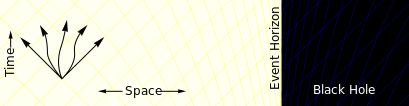
\includegraphics[width=0.7\textwidth]{img/Introd/1.png}\\
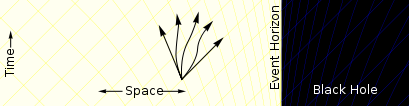
\includegraphics[width=0.7\textwidth]{img/Introd/2.png}\\
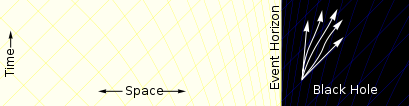
\includegraphics[width=0.7\textwidth]{img/Introd/3.png}
\end{tabular}
\caption{The figure shows how particles can move in any direction outside the event horizon but they can only move inwards the black hole once the event horizon is crossed.}
\label{blackholecones}
\end{figure}
The mathematically accurate version of this definition is more technical and involves the existence of a \textit{spacetime singularity}, which is a region of the spacetime where the movement of the particles that reaches this area cannot be extended, and an \textit{event horizon}, which is a surface that has the property to prevent the particles that cross this region to go back. We can understand this behavior with the use of the Minkowsky diagrams, that are plots in which the time coordinate is represented in the vertical axis and the space coordinate is represented in the horizontal axis. In these diagrams the trajectories of the photons are straight lines sloping at 45 degrees. As photons (null particles onwards) are the limit behavior of mass particles (timelike particles onwards), the last ones must remain inside the cone defined by the straight lines at 45 degrees. This is known as the ''light cone'' and can be used to study the regions of the spacetime that are accessible to physical particles (causal particles onwards). As we can see in \cref{blackholecones}, the light cones outside the event horizon allow causal particles to move in any direction, but closer to the horizon the spacetime starts to deform. There are more allowed movements going towards the horizon than moving away. Inside the event horizon causal particles are not allowed to escape from this region, as the spacetime is so bended that the only allowed behavior is moving towards the black hole. 

The black holes can be categorized in virtue of the ''no hair theorem'', which stipulates that these entities can be described with three properties: Mass, electromagnetic charge and angular momentum. With this information in mind, the black holes are named as
\begin{figure*}[hpt!]
\centerline{
\begin{tabular}{c|c|c}
 & Non-rotating ($L=0$) & Rotating ($L\neq0$) \\   \hline
 Uncharged ($Q=0$) & Schwarzschild &  Kerr \\   \hline
 Charged ($Q \neq 0$) & Reissner Nordstr\"om & Kerr-Newman
\end{tabular}
}
\end{figure*}

The complexity order is 
\begin{equation*}
 \text{Schwarzschild }\rightarrow \text{Reissner Nordstr\"om} \rightarrow \text{Kerr} \rightarrow \text{Kerr-Newman}.
\end{equation*}
As general relativity states, freefall particles in the spacetime must move along causal (timelike or lightlike) \textit{geodesics}, and therefore in order to understand the paths of these particles we must obtain and analyze the geodesics trajectories of the spacetime. In the \gls{SW} spacetime, the geodesic flow is well understood but its study still provides new and interesting results \cite{belbruno2011dynamical,marck1996short,galindo2014mcgehee}. In the \gls{RN} spacetime, the geodesic flow is much more complicated due to the fact that the spacetime structure is more complex and some features of the geodesics are still being analyzed nowadays \cite{galindo2014mcgehee}.
\begin{figure}[htp!]  
\begin{center}
 \centerline{\includegraphics[width=0.8\textwidth]{img/Introd/ZAMOS.png}}
 \end{center}
 \vspace{-1.5cm}
 \caption{Trajectories with zero angular momentum in the Kerr spacetime.}
 \label{fig:rotzam}
\end{figure}
The study of the Kerr spacetime is even more complex that in the \gls{RN} spacetime and the geodesic flow is very difficult to understand and analyze. Indeed, there are very intricate technical books dedicated to this topic \cite{o1995geometry} that do not even provide a general (either quantitatively or qualitatively) description for all possible geodesics. Due to its complexity, the Kerr metric is still an important research field because it is known that the spacetime described by every collapsing astrophysical object approaches the Kerr spacetime asymptotically, and therefore almost every black hole in the universe is a Kerr black hole (except those which also have charge, but as the charge is very low for common astrophysical objects). It is interesting to note that while the \gls{SW} and \gls{RN} geometries can be used to describe the exterior of a spherically symmetric object in virtue of the Birkhoff theorem \cite{birkhoff1923relativity}, the Kerr geometry only describes a black hole. For example, it is known that while the spacetime singularities in the \gls{SW} and \gls{RN} geometries are single points (that for mathematical reasons are not in the spacetime), the Kerr singularity is a topological ring. Also, one of the most popular features in the Kerr geometry is the \textit{frame dragging}. This phenomenon consists in the Kerr black hole dragging the fabric of spacetime itself in its movement and therefore, it also drags the trajectory of the physical particles moving in its presence. This effect can be so relevant, that there are some regions in the black hole known as \textit{ergoregions} where all the particles are forced to rotate in the same direction as the black hole does. Indeed, trajectories with zero angular momentum (that in the \gls{SW} and \gls{RN} spacetimes correspond to straight lines) are not straight lines but curved trajectories that spin co-rotating with the black hole as is depicted in \cref{fig:rotzam}.
\begin{figure}[hpt!]  
\begin{center}
 \centerline{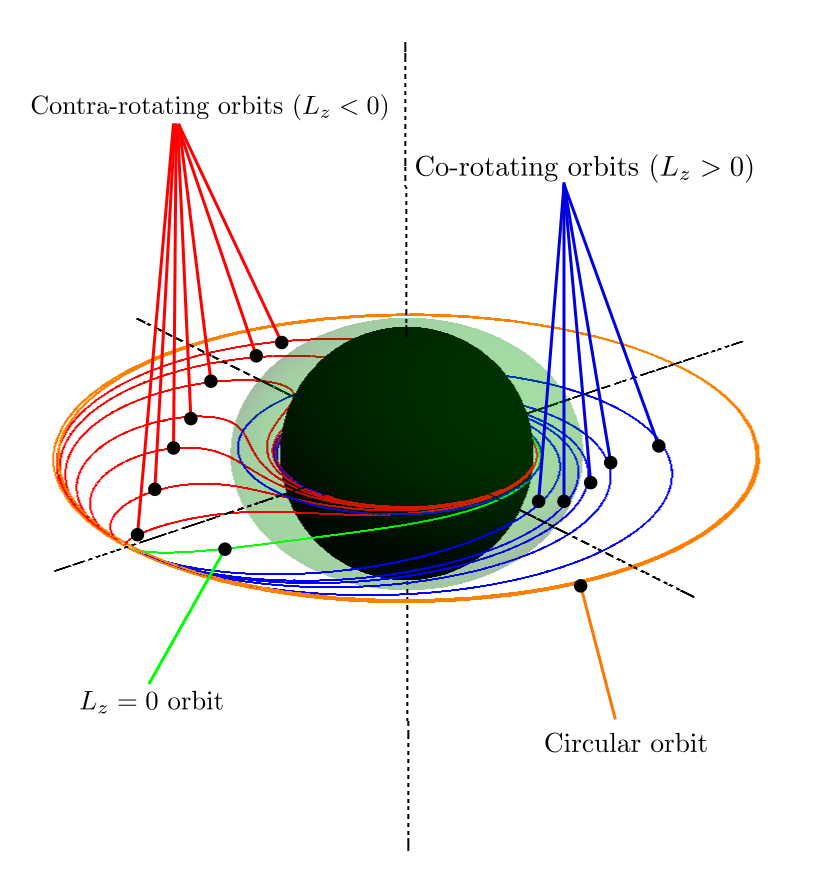
\includegraphics[width=0.7\textwidth]{img/Introd/Orbits.png}}
 \end{center}
 \vspace{-1.5cm}
 \caption{Behavior of timelike particles near a Kerr black hole. The black hole is rotating anticlockwise. The black region correspond to the event horizon while the green one correspond to the ergoregion. The orbits drawn red are retrograde geodesic that are spin-reversed by the black hole, the blue paths are direct geodesics, the orange curve is a circular orbit while the green one is the $L_z=0$ geodesic.}
 \label{fig:orbits}
\end{figure} 
All the possible behaviors are depicted in \cref{fig:orbits} where we can see how trajectories attempting to enter the ergoregion contra-rotating with respect to the black hole, are forced to spin in the same direction of the black hole. Also, particles with zero angular momentum are still moving in a co-rotating movement as well as particles with positive angular momentum. As also happens in the \gls{SW} and \gls{RN} geometries, particles with enough angular momentum can move in circular orbits around the Kerr black hole.

But there are features of the Kerr black holes even stranger than the frame dragging. The Kerr black hole has what is known as a Einstein - Rosen bridge or more typically as a \textit{wormhole}, which is a topological feature of the spacetime that connects two different regions (called sometimes ''universes'' in the literature) of the spacetime. In this case, the wormhole (which is located at the center of the ring singularity) leads to the \textit{negative space}, a region of the spacetime in which gravity is repulsive. In this space there also causal violations, i.e. there exist trajectories allowed to physical particles that lead to time travel. As the wormhole is inside the event horizon, these trajectories cannot be seen from outside the black hole. Thus, possible causality violations are ''protected'' by the event horizon. The maximal analytic extension of the Kerr black hole (which is the whole spacetime described by the Kerr metric) is even more complex and reveals that the Kerr black hole has an infinite amount of asymptotically flat regions and an infinite amount of wormholes that connects them. These wormholes are different from the wormholes that connect with the negative space.

As we can see, the structure of the spacetime is very complex and therefore, the description of the movement of physical particles in the Kerr geometry is very difficult to understand. The aim of this work is present a method that allows us to analyze the full motion of the particles in some regions of interest in the spacetime. Our main focus will be the use of dynamical systems, which have proven to be a powerful tool in the study and description of physical systems, as demonstrated by theoretical mechanics. The combination of General Relativity and dynamical systems is a very novel approach to the problem \cite{stoica1997schwarzschild,belbruno2011dynamical,galindo2014mcgehee} which describes certain known results from a completely new perspective. The two regions in which we are interested are the axis of symmetry and the equatorial plane. The axis of symmetry is a very important region because it contains the easiest way to travel to the negative space. The description of the geodesic flow in the axis of symmetry is a very difficult topic with the standard methods because a complete study of the geodesic flow involves the movement in an infinite amount of asymptotically flat regions and negative spaces. This is the reason why the current analysis of the geodesic flow in the axis is very difficult to understand and why it had remained incomplete. In this work, we achieve to describe the whole geodesic flow in the axis of symmetry by the use of a dynamical system technique that projects all the different trajectories into one two-dimensional phase portrait. This is a great simplification of this problem. The other region in which we are interested is in the equatorial plane, because it contains the ring singularity of the Kerr spacetime and the disk inside this singular ring, which is the wormhole that connects to the negative space. The analysis of the trajectories in the axis and in the equatorial plane is essential because allows us to understand some very important characteristics of the black holes as the jets or accretion disks. What is known as the Penrose process conforms a mechanism that allows us to understand the powerful jets that quasars and rotating black holes emit. This process involves expelled particles that gain energy while the black hole loses it, decreasing its own rotation. This is still one of many viable competing models for quasar jets.

Its important to warn that the Kerr metric describes an \textit{eternal black hole}, which has existed forever and therefore does not come from a collapsing astrophysical object. It is known that the Kerr black holes produced by the gravitational collapse probably will not have the infinite wormhol structure, as these wormholes are unstable and will collapse under small perturbations. However, the wormhole that leads to negative space is stable and probably will survive the gravitational collapse.

This work is organized as follows: In \cref{ch:KerrG} we present a brief but concise description of the Kerr spacetime and its main features. As we will see in this chapter we will need a new coordinate system that allow us to describe the geodesic flow in the whole spacetime without having to worry about  horizons or wormholes. In \cref{ch:introduction} we define the new coordinate system and we express all the quantities of interest in this new coordinates. Also, we show how the Kerr spacetime is described in the new coordinates and the main features of the important surfaces. In \cref{ch:MAE} perform a rigorous analysis of the topological identification describing the wormhole that lead to the negative space and we also describe how the new coordinates are very useful studying the movement in maximal extension, which is also examined in detail. In \cref{ch:dinamicsys} we performed a comprehensive study of the geodesic flow along the axis of symmetry in terms of dynamical systems, with particular attention to the causal structure and the stability of the motion along the axis. After that, a similar study about the equatorial plane is performed in \cref{ch:ep} with special emphasis in the disk inside the singular ring and its stability. Finally in \cref{ch:nsog} we display some interesting geodesic defined along the whole Kerr spacetime obtained by a numerical integration software developed for this work. Some useful information that completes the understanding of this work can be found in \cref{Killingchapter}.

\part{Development and results}
%************************************************
\chapter{The Kerr spacetime}\label{ch:KerrG}
%************************************************

Throughout all the work we will use natural units, so we will set the speed of light ($c=1$) and the universal gravitation constant ($G_N=1$). Notice that in this unit system the dimension of space and the dimension of time are equivalent. Also, the Penrose index notation will be used (the contravariant or covariant character of the tensors is described by the number of super-indexes and sub-indexes respectively). In this chapter we are going to display some interesting and basic features of the Kerr-Spacetime. All this features are well known and can be found with much more detail in the first Chapter of \cite{o1995geometry}. Despite this, we believe it is interesting to make a brief illustrative trip through the behaviors of the Kerr black hole as well as the features of the causal observers moving in the Kerr geometry in a suitable way for any reader with a basic knowledge of differential geometry and general relativity. As any other black hole, the Kerr black hole has an event horizon that prevents that any observer that cross this surface can go back and therefore ``protects'' the singularity. But in the Kerr spacetime the structure of the horizons (there is more than one) is more complicated that in the \gls{SW} geometry or the \gls{RN} geometry because in this case there is also a region called \textit{ergosurface}, in which particles cannot remain static, neither can rotate in the opposite direction of the black hole rotation, i.e. in this region the only allowed movement is to move co-rotating with the black hole. Also, as we will see, the Kerr true singularity cannot be understood in the standard coordinates (which are called \gls{BL} coordinates) and we will have to express the metric in another coordinate system to unveil the true nature of this singularity.

\section{The Kerr metric in Boyer-Lindquist coordinates}
The explicit form of the metric in \gls{BL} coordinates is
 \begin{align*}
 ds^2&=-d\bar{t}^2+ \Sigma \left(\frac{dr^2}{\Delta}+d\theta^2 \right)+(r^2+a^2)\sin^2{(\theta)} d\bar{\phi}^2\\
 &+\frac{2 M r}{\Sigma}(a \sin^2{(\theta)} d \bar{\phi} -d\bar{t})^2
\end{align*}
where
\begin{align}
 \Delta(r)&=r^2-2Mr+a^2\\
 \Sigma(r,\theta)&=r^2+a^2 \cos^2 \theta
\end{align}
The \gls{BL} coordinates are form by the tetrad $\{\bar{t},r,\theta,\phi\}$ which takes values on $\bar{t}\in \mathbb{R}$, $r \in \mathbb{R}^+$ , $\{\theta,\phi \} \in S^1$. The Kerr metric depends on two parameters, $M$ and $a$. If we compare the metric with the far field metric generated by an isolated object we can deduce that these parameters are respectively the mass and the angular momentum per unit of mass of the black hole, both measured at the infinity. Some properties of the Kerr black hole arise from the properties of the metric:
\begin{enumerate}
 \item The Kerr metric is stationary, which means that the metric it does not depend explicitly on the coordinate $\bar t$ that yields the (asymptotic) time..
 \item The Kerr metric is axisymmetric, which means that the metric does not depend on the $\phi$ coordinate.
 \item The Kerr metric is not static because it is not invariant under the time reversal transformation $\bar{t} \rightarrow -\bar{t}$
 \item The Kerr metric is invariant under the transformation
 \begin{align}
  \bar{t} & \rightarrow -\bar{t}\\
  \phi & \rightarrow - \phi
 \end{align}
this can be interpreted as the time reversal of the Kerr metric produces a black hole that is rotating in the opposite direction.
\item Is asymptotically flat, which means that in the limit $r \to \infty$ the Kerr metric becomes the Minkowsky metric in spherical coordinates.
\item In the limit $a \to 0$ the Kerr metric becomes the \gls{SW} metric in Droste coordinates.
\item In the limit $M \to 0$ (but $a \neq 0$) the Kerr metric becomes isometric to the Minkowsky spacetime in spherical coordinates.
\end{enumerate}

\section{Symmetries}

As we notice before, the Kerr metric has two important symmetries because its stationary and axisymmetric. Therefore, the Kerr metric admits two Killing vector fields (to know more about Killing vectors, see \vref{Killingchapter})
\begin{equation}\label{killvec}
 \xi_1= \partial_t \quad \quad \quad \xi_2=\partial_\phi.
\end{equation}
If we name $u^\alpha$ to the geodesics tangent vector, there exist two conserved quantities associated with this Killing vectors:
\begin{align}\label{conserved11}
 -E = u^\alpha {\xi_1}_\alpha \quad \quad \quad L_z=u^\alpha {\xi_2}_\alpha
\end{align}
In the case of timelike geodesic these conserved quantities can be interpreted as the energy per unit of mass of the particle measured at the infinity and the angular momentum per unit of mass measured at the infinity. In the case of null geodesics this interpretation can be maintained if we parametrize the geodesic flow with the affine parameter of the geodesic. In the following, this convention will be maintained. 

\section{The curvature}
  \begin{figure}[htp!]  
\begin{center}
 \centerline{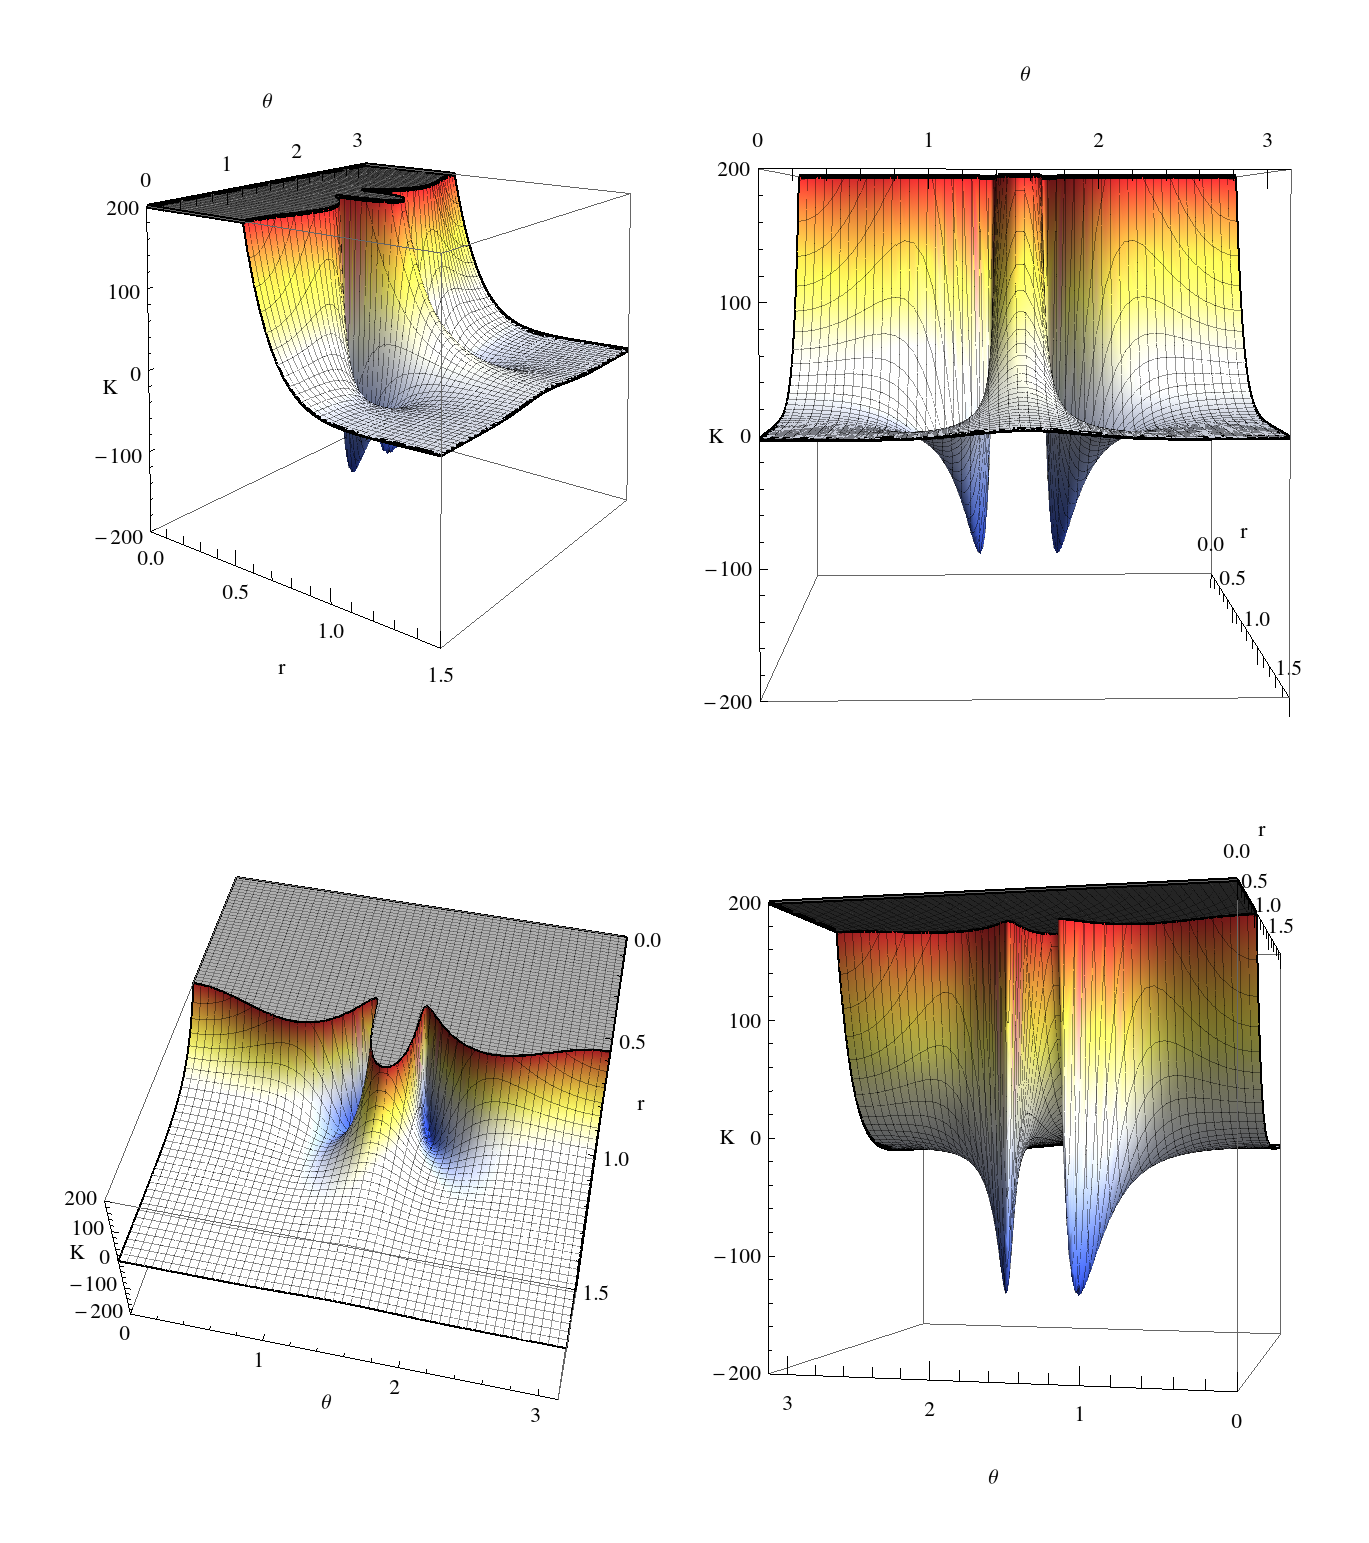
\includegraphics[width=1\textwidth]{img/Chapter0/Kresch.png}}
 \end{center}
 \vspace{-1.5cm}
 \caption{The figure shows the variation of the Kretschmann invariant as a function of the variables $r$ and $\theta$ of the \gls{BL} coordinates. The grey region indicates  the cut-off of the surface which continues to higher values. $M=1$ and $a=0.9$ has been chosen for illustrative purposes.}
 \label{fig:Kresch}
\end{figure} 
The curvature scalar is usually defined by the Riemann scalar
\begin{equation}
 R=Ric^{\alpha}_{\,\alpha}
\end{equation}
where $Ric_{\alpha \beta}=R^\gamma_{\,\alpha \gamma \beta}$ and $R^{\alpha}_{\,\beta \gamma \delta}$ is the Riemann tensor. However the scalar $R$ vanishes because the Kerr solution corresponds to a solution of the vacuum Einstein equations. The Einstein equations without cosmological constant are
\begin{equation}
 Ric_{\alpha \beta}-\frac{1}{2} g_{\alpha \beta} R=T_{\alpha \beta}
\end{equation}
where $T_{\alpha \beta}$ is the Energy-Stress tensor. Taking the trace of the equations we get
\begin{equation}
 -R=T
\end{equation}
where $T=T^\alpha_{\,\alpha}$. As for the vacuum Einstein field equations we have that $T_{\alpha \beta}=0$ then $R=0$ and therefore the curvature scalar does not give any information of the spacetime curvature. But we can construct other invariant quantities with the Riemann tensor. One of the most important ones is the invariant $K=R_{\alpha \beta \gamma \delta}R^{\alpha \beta \gamma \delta}$, which is known as the Kretschmann invariant. As any other invariant, its properties does not depend of the choice of the coordinate system. A direct computation of the Kretschmann invariant in \gls{BL} coordinates gives
\begin{equation}
 K=R_{\alpha \beta \gamma \delta}R^{\alpha \beta \gamma \delta}=\frac{8 \left(6 M^2 \left(-a^6 \cos ^6(\theta )+15 a^4 \cos ^4(\theta )-15 a^2 r^4 \cos ^2(\theta )+r^6\right)\right)}{\left(a^2 \cos ^2(\theta )+r^2\right)^6}
\end{equation}
The variation of $K$ as a function of $r$ and $\theta$ is depicted in \cref{fig:Kresch}. Notice that there exist regions with negative curvature, which means that in this region the Riemann tensor is fundamentally timelike, which can only happen in Lorenzian manifolds. We see that the curvature becomes infinite iff
\begin{equation}
a^2 \cos ^2(\theta )+r^2= 0 \rightarrow r=0 \quad \quad \mbox{and} \quad \quad \theta=\frac{\pi}{2},
\end{equation}
which is the only true spacetime singularity.

\section{Singularities and horizons}

The Kerr metric has some interesting properties that concern spacetime singularities. Some of these singularities are not really there, as they are which is known as \textit{Coordinate singularities}, that are points where the expression of the metric element becomes singular but due to a bad election of the coordinate system. Although this may seem only a problem of the coordinate system, these singularities are much more interesting, because they reveal some interesting causal properties of the Kerr spacetime. We can see that the Kerr metric is singular when
\begin{align}
 \Delta &=0,\\
 \Sigma&=0.
\end{align}
We will name these equations \textit{singularity equations}. The singularities of the first equation (namely $r=r_\pm$) correspond to a pair of \textit{coordinate singularities} as the computation of the Kretschmann invariant $R_{\alpha \beta \gamma \delta}R^{\alpha \beta \gamma \delta}$ (where $R$ is the Riemann tensor) suggests that these points are not truly spacetime singularities and we call them \textit{horizons}. On the other hand the singularity of the second equation is really a spacetime singularity as we have seen in the last section.

The coordinate singularities given by $\Delta=0$ are located at
\begin{equation}
 r=r_\pm=M \pm \sqrt{M^2-a^2}
\end{equation}
When $a^2<M^2$ the two solutions of the singularity equation exist but when $a^2=M^2$ they become one solution as $r_+=r_-=M$. For values of the angular momentum of the black hole that fulfill $a^2>M^2$ there is no real solution to the singularity equation and therefore no horizons exist. In this situation the Kerr solution does not describe a black hole, as the spacetime singularity is not covered by any event horizon, which will lead to paradoxes. This is the reason that all astrophysical processes are believed to lead to black holes with $a^2 \leq M^2$. When $|a|=|M|$ the Kerr spacetime is called \textit{extremal black hole} and for values of $a$ and $M$ such that $|a|>|M|$ the black hole is called \textit{superextreme black hole}. Let us consider now the normal 1-form to the constant-$r$ hypersurfaces which is given in  \gls{BL} coordinates as
\begin{equation}
 n_\alpha=(0,1,0,0)
\end{equation}
By the use of the Kerr metric we can evaluate its norm as
\begin{equation}
 n^\alpha n_\alpha= n^\alpha n^\beta g_{\alpha \beta} = \frac{\Delta}{\Sigma}.
\end{equation}
We can see that on the horizons ($r=r_\pm$) $n^\alpha n_\alpha=0$ which reveal that they are null hypersurfaces, and this is because they are called horizons. The two horizons separate the structure of the spacetime in three regions
\begin{enumerate}
 \item The region in which $r>r_+$. In this region the constant-$r$ surfaces have timelike causal character and as in the limit $r \to \infty$ the metric becomes the Minkowsky metric, we say that this is the exterior of the black hole.
 \item The region in which $r_-<r<r_+$ the constant-$r$ surfaces have spacelike causal character. A deeper analysis of the causal structure tell us that an object that falls through $r=r_+$ can only continue falling until it reaches $r=r_-$. This is the reason we call $r=r_+$ the event horizon.
 \item The region in which $r<r_-$ the constant-$r$ surfaces are timelike again and this is the region that contains the spacetime singularity.
\end{enumerate}
Notice that in the range $a^2 \geq M^2$ the second region does not exist and when $a^2>M^2$ the 1st and 3rd regions are causally connected because there is no horizon that prevent this behavior.

Notice that the spacetime singularity is located at $r=0$ and $\theta=\frac{\pi}{2}$ (but no at $r=0$ and $\theta \neq \frac{\pi}{2}$).This relation has no meaning in spherical-like coordinates (the \gls{BL} coordinates). We need another coordinate system to reveal the true shape and properties of the spacetime singularity. In the next chapter, we will see that in another well-behaved coordinate system, the Kerr singularity happens to be a ring that increases it radius with the value of $a$, being a single point when $a=0$.

\section{ZAMOS}
  \begin{figure}[htp!]  
\begin{center}
 \centerline{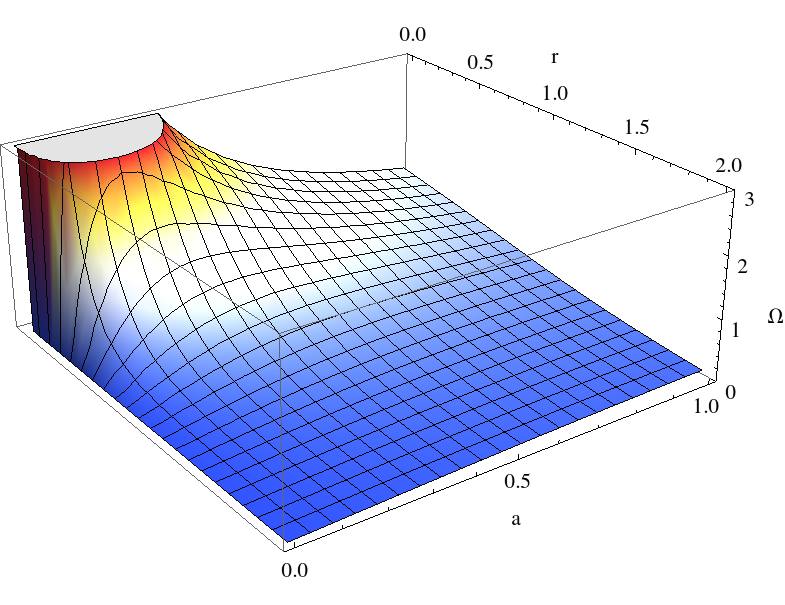
\includegraphics[width=0.8\textwidth]{img/Chapter0/ZAMO.png}}
 \end{center}
 \caption{The figure shows the ZAMO angular velocity $\Omega$ in de equatorial plane ($\theta=\frac{\pi}{2}$). The color is proportional to the value of $\Omega$ (that is in the vertical axis also) and it is only for improve the visualization.}
 \label{fig:ZAMO}
\end{figure} 
We are going to study one of the most popular Kerr features, that is the frame dragging. Remember that a Newtonian observer in a axisymmetric potential (or even an observer in the \gls{SW} or \gls{RN} geometries) in freefall has a radial trajectory if $L_z=0$. This is because the radial velocity is proportional to the angular momentum $L_z$. To study what happens in the Kerr spacetime, let us consider an observer with zero angular momentum. In virtue of \cref{conserved11} we can write
\begin{equation}\label{zamoeq1}
 L_z=u_{\bar{\phi}}=0
\end{equation}
In the literature, this observer is commonly known as \gls{ZAMO}. Notice that the contravariant component of the velocity is
\begin{equation}
 u^{\bar{\phi}}=g^{\bar{\phi} \bar{t}}u_{\bar{t}} \neq 0
\end{equation}
and therefore the \gls{ZAMO} can, in principle, have radial component in the tangent vector and therefore its trajectory will not be a radial movement. From \cref{zamoeq1} we can write
\begin{equation}
 u_{\bar{\phi}}=g_{\bar{\phi} \bar{\phi}}u^{\bar{\phi}} + g_{\bar{\phi} \bar{t}} u^{\bar{t}}=0
\end{equation}
and therefore the angular velocity of the \gls{ZAMO} is given by
\begin{equation}
 \Omega=\frac{u^{\bar{\phi}}}{u^{\bar{t}}}=-\frac{g_{\bar{\phi} \bar{t}}}{g_{\bar{\phi} \bar{\phi}}}=\frac{2 M a r}{(r^2+a^2)^2-a^2 \Delta sin^2\theta}.
\end{equation}
The \cref{fig:ZAMO} shows the behavior of this function in the equatorial plane (the behavior is similar for other values of $\theta$). Notice that as the denominator is always positive then
\begin{equation}
 sign(\Omega)=sign(M a)
\end{equation}
and therefore the \gls{ZAMO} rotates in the same direction as the black hole. We conclude two important results:
\begin{itemize}
 \item Observers with zero angular momentum cannot move in radial movements (straight lines) .
 \item An observer which approaches a Kerr black hole with zero angular momentum is dragged by the gravitational force of the black hole and the only movement allowed is rotate in the same direction as the black hole.
\end{itemize}
  \begin{figure}[htp!]  
\begin{center}
 \centerline{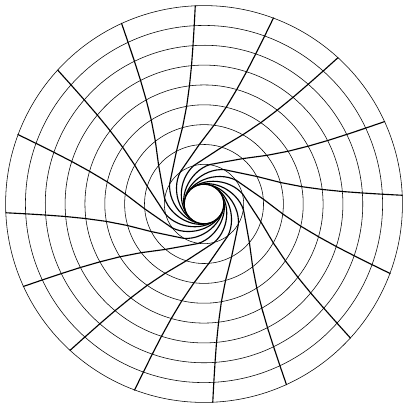
\includegraphics[width=0.6\textwidth]{img/Introd/Dragg.png}}
 \end{center}
 \caption{Frame dragging in the Kerr spacetime. }
 \label{fig:Dragg}
\end{figure} 
The effect of the frame dragging over the \gls{ZAMO}s can be visualized in \cref{fig:Dragg}, where we can see how the trajectories with $L_z=0$ (that are straight lines in the infinity as $\lim_{r\to\infty} \Omega=0$) are dragged by the Kerr black hole. We will see that the frame dragging is even more strong and complex that that and has a very important role in what is known as the ergoregions.

\section{The ergosphere}

In the \gls{SW} geometry it is known that the Killing vector $\partial_{\bar{t}}$ is timelike outside the even horizon (remember that in the \gls{SW} geometry there is only one horizon), null over the horizon and spacelike inside the horizon. That is why it is said that inside the horizon the coordinate $\bar{t}$ measures space while the coordinate $r$ measures time. as the \gls{SW} singularity is located at $r=0$ and as inside the horizon $r$ measures time, its said that the \gls{SW} singularity its not a place but a time: \textit{The singularity is not there but it is tomorrow}. This can be easily understood if you think that tomorrow the universe reachable by you is supposed to disintegrate and disappear. This is what "hitting" the \gls{SW} singularity is not a "place", it is everywhere in the future. However, in the Kerr spacetime the singularity is located at $r=0$, and in this region $r$ is a spacelike coordinate and therefore the singularity in really a ''place'', not a moment in time. In the Kerr geometry, the points where the Killing vector changes its spacetime causal character (timelike, null or spacelike) do not match with the singularities (coordinate singularities) of the metric. As the causal character of the Killing vector is given by$g(\partial{\bar{t}},\partial{\bar{t}})=g_{tt}$ we can see where the component $g_{tt}$ changes its sign. We write
\begin{equation}
 g_{tt}=-1+\frac{2M r}{\Sigma}=\frac{r^2-2M r+a^2 \cos^2 \theta}{\Sigma}=0.
\end{equation}
This equation has two solutions
\begin{equation}
 r_{E\pm}=M \pm \sqrt{M^2-a^2 \cos^2\theta}.
\end{equation}
These two solutions are known as the \textit{ergosurfaces} and also as the \textit{infinity redshift surfaces}. The reason of the second name is that if we think in a light source located on a point $p_s$ that emits a light pulse with frequency $\nu_s$ it will be observed with frequency
\begin{equation}
 \nu_{\text{obs}}=\sqrt{\frac{g_{tt}(p_s)}{g_{tt}(p_\text{obs})}}  \nu_s
\end{equation}
(where $ \nu_{\text{obs}}$ is the frequency measured by an observator located at the point $p_\text{obs}$) and therefore the observed frequency is $ \nu_{\text{obs}}=0$ if the light pulse is emitted from $p_s=r_{E \pm}$ because $g_{tt}(r_{E \pm})=0$. Let us call $\mathcal{I}=[r_{E-},r_{E+}]$, the interval between the two ergosurfaces. Notice that the two horizons are always in this interval ($r_\pm \in \mathcal{I}$) as
\begin{equation}
 r_- \leq r_{E-} \leq r_{E+} \leq r_+.
\end{equation}
  \begin{figure}[htp!]  
\begin{center}
 \centerline{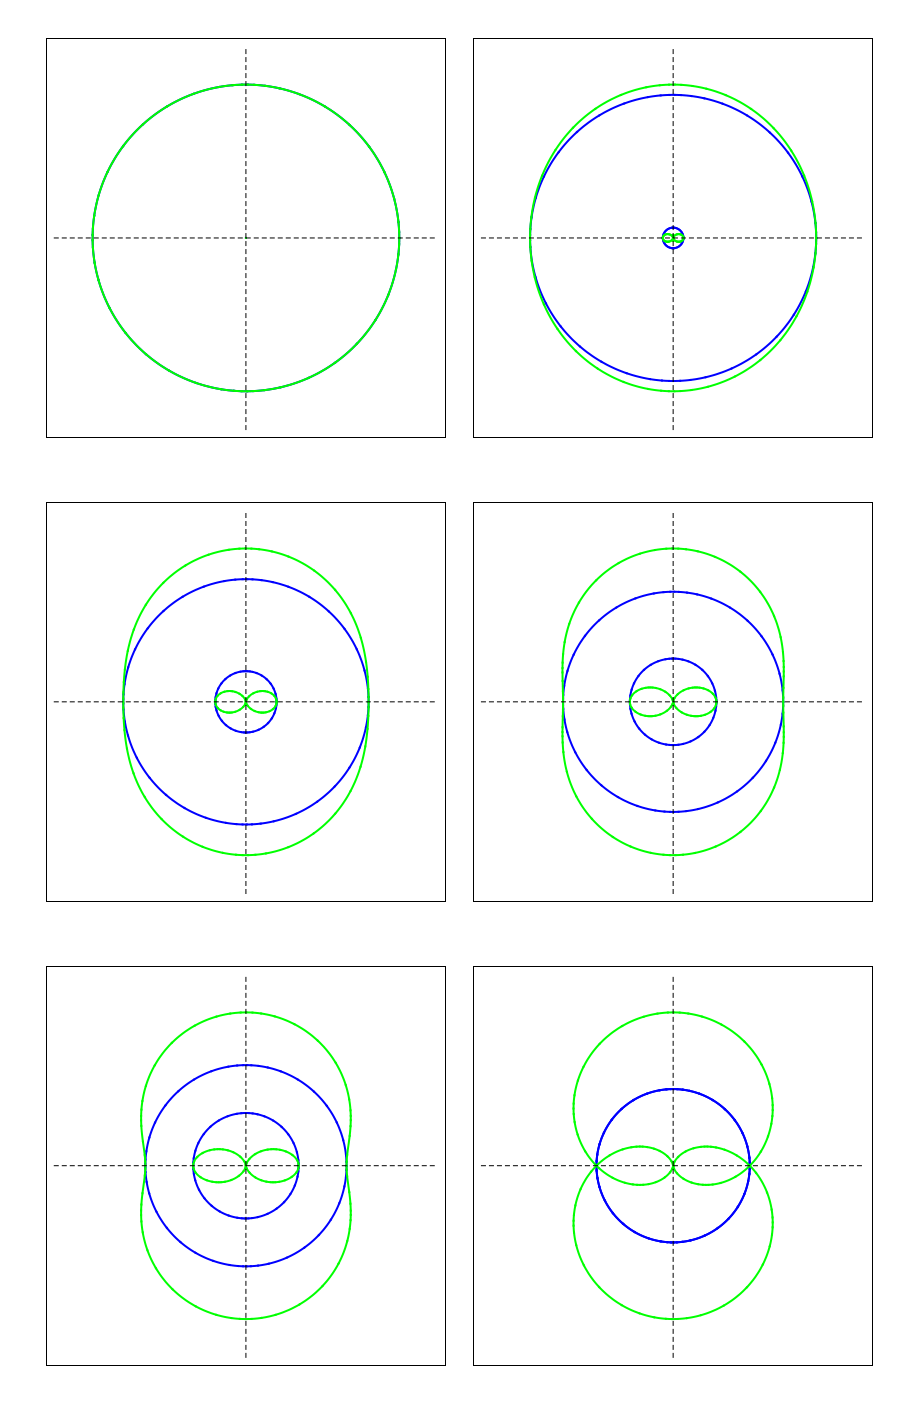
\includegraphics[width=0.95\textwidth]{img/Chapter0/erg.png}}
 \end{center}
 \vspace{-1.5cm}
 \caption{Schematic location of the horizons, ergosurfaces, and curvature singularity in the side view of the Kerr Spacetime in \gls{BL} coordinates as a function of the parameter $a$. The images correspond to (from left to right and from top to bottom) $a=0$,$a=0.5$,$a=0.8$,$a=0.9$,$a=0.95$,$a=1$. The green surfaces are the outer and inner ergosurfaces and the blue curves represent the inner and outer horizon. Notice that the singularity is at the center of the image ($r=0$ $\theta=\frac{\pi}{2}$). For simplicity $M=1$ is chosen.}
 \label{fig:ergo1}
\end{figure} 
In \cref{fig:ergo1}, a schematic image of the horizon and ergosurfaces is displayed. Given these results, we have have that $g_{tt}<0$ iff $r \notin \mathcal{I}$ and $g_{tt}>0$ iff $r \in \mathcal{I}$. Therefore, there is a region between the outer horizon and the outer ergosurface where $g_{tt}>0$ (this does not happen in the \gls{SW} spacetime). This region is known as the \textit{ergoregion} and $r=r_{E+}$ is called  \textit{ergosphere}. Its very important that the ergoregion exists outside the outer horizon, because this fact allows a geodesic that comes from the asymptotically flat region enter the ergoregion and escape to the asymptotically flat region again (without being trapped by the black hole as the geodesic does not cross the even horizon). As $g_{tt}>0$ in this region, the Killing vector becomes spacelike. Some strange features happen in this region. First of all, as the conserved quantity of the $\partial_{\bar{t}}$ Killing vector is $ u^\alpha {\xi_1}_\alpha=-E$ and as $\xi_1$ is spacelike, $E$ can be negative as well. Negative energies are only allowed inside the horizon in the \gls{SW} geometry, as in the \gls{RN} geometry (that is the \gls{SW} spacetime with charge in the source of the gravitational field). The main strange feature is that there is no stationary observers allowed in the ergoregion. An stationary observer is an observer which does not see the metric change in its motion. For example, a observer in $\partial_t$, which is an observer that does not change the coordinates $\{r,\theta,\phi\}$ (and therefore its tangent vector must be proportional to $\partial_{\bar{t}}$) is an example of a stationary observer. As stationary observers does not see the metric change in its motion, and we know that the metric does not change along the trajectories of the Killing vectors, the tangent vector to the geodesic of the stationary observer must be a Killing vector, i.e. a linear combination of the independent Killing vector fields in \cref{killvec}. As the observers in the spacetime must move along causal timelike curves ($u^\alpha u_\alpha =-1$, where $u^\alpha$ is the tangent vector to the trajectory) we can see that observers in $\partial_t$ (those whose tangent vector is proportional to $\partial_{\bar{t}}$) are not allowed in the ergoregion because in this region $\partial_{\bar{t}}$ is spacelike and therefore only stationary observers whose tangent vector is a linear combination of the two Killing vectors are allowed. To understand what this means we are going to compute the unitary tangent vector of a general stationary observer as
\begin{equation}
 u^\alpha=\frac{\partial_{\bar{t}}+\omega \partial_\phi}{|\partial_{\bar{t}}+\omega \partial_\phi|}=(u^t,0,0,u^\phi)=u^t(1,0,0,\omega),
\end{equation}
where we have defined $\omega$ as
\begin{equation}
 \omega= \frac{d \phi}{d \bar{t}}=\frac{u^\phi}{u^t},
\end{equation}
to be the constant angular velocity of the observer. As we see, the trajectory of the observer has constant $r$ and $\theta$ coordinates and can only move along a circle with angular velocity $\omega$. Observer's tangent vectors must fulfill
\begin{equation}\label{conditionob}
 u^\alpha u_\alpha=(u^t)^2 \left( g_{tt}+ 2 \omega g_{t \phi}+ \omega^2 g_{\phi \phi} \right) =-1 \rightarrow  g_{tt}+ 2 \omega g_{t \phi}+ \omega^2 g_{\phi \phi}<0.
\end{equation}
To understand this equation, let us solve
\begin{equation}
  g_{tt}+ 2 \omega g_{t \phi}+ \omega^2 g_{\phi \phi}=0.
\end{equation}
The solutions of this equation are
\begin{equation}
 \omega_{\pm}=\frac{-g_{t\phi} \pm \sqrt{g_{t \phi}^2- g_{tt} g_{\phi \phi}} }{g_{\phi \phi}}.
\end{equation}
Notice that the discriminant of the equation is $g_{t \phi}^2- g_{tt} g_{\phi \phi}=\Delta \sin^2 \theta$ and therefore this equation has no real solutions for $\Delta <0 $ which implies $r_-<r<r_+$. This has the meaning that no stationary observers are allowed when  $r_-<r<r_+$ . Outside the outer horizon $r>r_+$ we have that $\Delta>0$ and the inequality \cref{conditionob} is satisfied when
\begin{equation}
 \omega_- <\omega <\omega_+.
\end{equation}
As we have that in the ergosphere ($r=r_{E+}$) $\omega_-(r=r_{E+})=0$ as $g_{tt}=0$ in this surface, then for $r \geq r_{E+}$ we will have $\omega_- \leq 0$ and the stationary observer can spin contra-rotating with the black hole ($\omega<0$) or co-rotating with the black hole ($\omega>0$). For $r_+<r<r_{E+}$ we have that $\omega_->0$ and therefore the observer can only rotate co-rotating with the black hole. This can be summarized as
\begin{enumerate}
 \item There is no stationary observer in the region $r_-<r<r_+$ .
 \item When a particle is in the ergoregion ($r_+<r<r_{E+}$, it can only move spinning co-rotating with the black hole and it cannot remain static (constant $\{r,\phi,\theta\}$ at the same time).
 \item Outside the ergoregion ($r \geq r_{E+}$ ) particles can move co-rotating or contra-rotating and observers in $\partial_t$ are allowed.
\end{enumerate}

Notice that as only photons (null causal curves) are allowed to move in the outer horizon $(r=r_+)$ and in this region $\omega_-=\omega_+$, then the only angular velocity of a null stationary observer is $\omega=\omega_\pm=\frac{2 M a r_+}{(r_+^2 + a^2)^2}=\frac{a}{r_+^2+a^2}=\Omega$, which is also the \gls{ZAMO} angular velocity. As this angular velocity is constant we can say that the black hole \textit{rotates rigidly}. This is because the angular velocity of the only curves that can remain in $r=r_+$ (that are null causal geodesic with its tangent vector given by $u^\alpha=(u^t,0,0,u^\phi)$ with $u^\alpha u_\alpha=0$) does not depend on the value of any coordinate.

\section{The Penrose process}
  \begin{figure}[htp!]  
\begin{center}
 \centerline{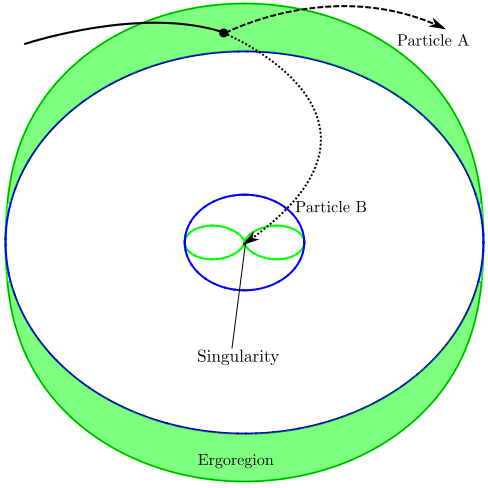
\includegraphics[width=0.4\textwidth]{img/Chapter0/Penrose.png}}
 \end{center}
 \caption{The figure shows the Penrose process in \gls{BL} coordinates. The green curves represent the inner and outer ergosphere and while the blue ones are the outer and inner horizons. Remember that in this coordinate system the singularity is located at $r=0$. For illustrative purposes $a=0.8$ and $M=1$ is chosen.}
 \label{fig:penroprocc}
\end{figure} 
The ergosphere has another very interesting feature: The Penrose process. As we have seen, the energies in the ergosphere can be negative $(E<0)$ as the Killing is spacelike in this region. Let us consider a particle that follows a geodesic that comes from the asymptotically flat region and then enters the ergosphere. Under some specific circumstances circumstances can decay into two particles A and B between the ergosphere and the outer horizon (this region is called ergoregion). The decay can be done in such a way that the particle B falls into the singularity, passing through the outer horizon, the inner horizon and the inner ergosphere and the particle B escapes to the asymptotically flat region. If the ingoing particle has energy $E$ and the two particles have energies $E_A$ and $E_B$ respectively, the global energy conservation allow us to write
\begin{align}
E&=E_A+E_B,\\
 E_\text{Kerr initial} + E&= E_\text{Kerr final}+E_A.
\end{align}
Particle B, crossing the event horizon, has a negative energy because within the ergosphere, the Killing vector $\partial_{\bar{t}}$ is spacelike and negative energies are allowed (remember that $g(\partial_t,u^\alpha)=-E0$, where $-E<0$ in the ergoregion). Then, as the total energy is conserved, the black hole absorbs a negative energy. The particle A that goes to infinity will gain that amount of energy because of the energy conservation $E_A>E$. Notice that as this process occurs at $r>r_+$ the particle A can return to the asymptotically flat region with more energy and therefore this act like a ''generator'', because we sent a particle with energy $E$ and we have gained a particle with energy $E_A>E$. The global result is that the Kerr black hole decelerates its rotation since it has absorbed negative energy. Blandford and Znajek (1977) suggested that the Penrose process could be a characteristic feature of Kerr black holes surrounded by a accretion disk containing a strong magnetic field. If this magnetic fields penetrates the ergoregion, then it could be a realistic source of electrons and positrons (created in pairs) which could start the Penrose process. This scenario involves that one of the particles end up with negative energy and falls into the black hole, while the other escapes to the asymptotically flat region. This second particle might form the characteristic energetic jets of charged particles that are known to be emitted from Kerr black holes, especially in quasars. By this process, quasar jets are powered by the energy that they extract from the Kerr black hole.



%************************************************
\chapter{Introduction}\label{ch:introduction}
%************************************************
This bundle for \LaTeX\ has two goals:
\begin{enumerate}
    \item Provide students with an easy-to-use template for their
    Master's
    or PhD thesis. (Though it might also be used by other types of
    authors
    for reports, books, etc.)
    \item Provide a classic, high-quality typographic style that is
    inspired by \citeauthor{bringhurst:2002}'s ``\emph{The Elements of
    Typographic Style}'' \citep{bringhurst:2002}.
    \marginpar{\myTitle \myVersion}
\end{enumerate}
The bundle is configured to run with a \emph{full} 
MiK\TeX\ or \TeX Live\footnote{See the file \texttt{LISTOFFILES} for
needed packages. Furthermore, \texttt{classicthesis} 
works with most other distributions and, thus, with most systems 
\LaTeX\ is available for.} 
installation right away and, therefore, it uses only freely available 
fonts. (Minion fans can easily adjust the style to their needs.)

People interested only in the nice style and not the whole bundle can
now use the style stand-alone via the file \texttt{classicthesis.sty}.
This works now also with ``plain'' \LaTeX.

As of version 3.0, \texttt{classicthesis} can also be easily used with 
\mLyX\footnote{\url{http://www.lyx.org}} thanks to Nicholas Mariette 
and Ivo Pletikosić. The \mLyX\ version of this manual will contain
more information on the details.

This should enable anyone with a basic knowledge of \LaTeXe\ or \mLyX\ to
produce beautiful documents without too much effort. In the end, this
is my overall goal: more beautiful documents, especially theses, as I
am tired of seeing so many ugly ones.

The whole template and the used style is released under the
\acsfont{GNU} General Public License. 

If you like the style then I would appreciate a postcard:
\begin{center}
 André Miede \\
 Detmolder Straße 32 \\
 31737 Rinteln \\
 Germany
\end{center}
The postcards I received so far are available at:
\begin{center}
 \url{http://postcards.miede.de}
\end{center}
\marginpar{A well-balanced line width improves the legibility of
the text. That's what typography is all about, right?}
So far, many theses, some books, and several other publications have 
been typeset successfully with it. If you are interested in some
typographic details behind it, enjoy Robert Bringhurst's wonderful book.
% \citep{bringhurst:2002}.

\paragraph{Important Note:} Some things of this style might look
unusual at first glance, many people feel so in the beginning.
However, all things are intentionally designed to be as they are,
especially these:
\begin{itemize}
    \item No bold fonts are used. Italics or spaced small caps do the
    job quite well.
    \item The size of the text body is intentionally shaped like it
    is. It supports both legibility and allows a reasonable amount of
    information to be on a page. And, no: the lines are not too short.
    \item The tables intentionally do not use vertical or double
    rules. See the documentation for the \texttt{booktabs} package for
    a nice discussion of this topic.\footnote{To be found online at 
    \url{http://mirror.ctan.org/macros/latex/contrib/booktabs/}.}
    \item And last but not least, to provide the reader with a way
    easier access to page numbers in the table of contents, the page
    numbers are right behind the titles. Yes, they are \emph{not}
    neatly aligned at the right side and they are \emph{not} connected
    with dots that help the eye to bridge a distance that is not
    necessary. If you are still not convinced: is your reader
    interested in the page number or does she want to sum the numbers
    up?
\end{itemize}
Therefore, please do not break the beauty of the style by changing
these things unless you really know what you are doing! Please.

\paragraph{Yet Another Important Note:} Since \texttt{classicthesis}'
first release in 2006, many things have changed in the \LaTeX\ world. 
Trying to keep up-to-date, \texttt{classicthesis} grew and evolved 
into many directions, trying to stay (some kind of) stable and be 
compatible with its port to \mLyX. However, there are still many 
remains from older times in the code, many dirty workarounds here and 
there, and several other things I am absolutely not proud of (for 
example my unwise combination of \acsfont{KOMA} and 
\texttt{titlesec} etc.).
\graffito{An outlook into the future of \texttt{classicthesis}.}

Currently, I am looking into how to completely re-design and 
re-implement \texttt{classicthesis} making it easier to maintain and 
to use. As a general idea, \texttt{classicthesis.sty} should be 
developed and distributed separately from the template bundle itself. 
Excellent spin-offs such as \texttt{arsclassica} could also be 
integrated (with permission by their authors) as format configurations. 
Also, current trends of \texttt{microtype}, \texttt{fontspec}, etc. 
should be included as well. As I am not really into deep 
\LaTeX\ programming, 
I will reach out to the \LaTeX\ community for their expertise and help.


\section{Organization}
A very important factor for successful thesis writing is the
organization of the material. This template suggests a structure as
the following:
\begin{itemize}
    \marginpar{You can use these margins for summaries of the text
    body\dots}
    \item\texttt{Chapters/} is where all the ``real'' content goes in
    separate files such as \texttt{Chapter01.tex} etc.
 %  \item\texttt{Examples/} is where you store all listings and other
 %  examples you want to use for your text.
    \item\texttt{FrontBackMatter/} is where all the stuff goes that
    surrounds the ``real'' content, such as the acknowledgments,
    dedication, etc.
    \item\texttt{gfx/} is where you put all the graphics you use in
    the thesis. Maybe they should be organized into subfolders
    depending on the chapter they are used in, if you have a lot of
    graphics.
    \item\texttt{Bibliography.bib}: the Bib\TeX\ database to organize
    all the references you might want to cite.
    \item\texttt{classicthesis.sty}: the style definition to get this
    awesome look and feel. Does not only work with this thesis template
    but also on its own (see folder \texttt{Examples}). Bonus: works
    with both \LaTeX\ and \textsc{pdf}\LaTeX\dots and \mLyX.
    \item\texttt{ClassicThesis.tcp} a \TeX nicCenter project file.
    Great tool and it's free!
    \item\texttt{ClassicThesis.tex}: the main file of your thesis
    where all gets bundled together.
    \item\texttt{classicthesis-config.tex}: a central place to load all 
    nifty packages that are used. %In there, you can also activate 
    %backrefs in order to have information in the bibliography about 
    %where a source was cited in the text (\ie, the page number).
    
    \emph{Make your changes and adjustments here.} This means that you  
    specify here the options you want to load \texttt{classicthesis.sty} 
    with. You also adjust the title of your thesis, your name, and all 
    similar information here. Refer to \autoref{sec:custom} for more 
    information.
    
        This had to change as of version 3.0 in order to enable an easy 
        transition from the ``basic'' style to \mLyX.
    
\end{itemize}
In total, this should get you started in no time.


\clearpage
\section{Style Options}\label{sec:options}
There are a couple of options for \texttt{classicthesis.sty} that
allow for a bit of freedom concerning the layout:
\marginpar{\dots or your supervisor might use the margins for some
    comments of her own while reading.}
\begin{itemize}
    \item General:
        \begin{itemize}
            \item\texttt{drafting}: prints the date and time at the bottom of
    each page, so you always know which version you are dealing with.
    Might come in handy not to give your Prof. that old draft.
        \end{itemize}
    
    \item Parts and Chapters:
        \begin{itemize}
            \item\texttt{parts}: if you use Part divisions for your document,
    you should choose this option. (Cannot be used together with 
    \texttt{nochapters}.)
    
            \item\texttt{nochapters}: allows to use the look-and-feel with 
    classes that do not use chapters, \eg, for articles. Automatically
    turns off a couple of other options: \texttt{eulerchapternumbers}, 
    \texttt{linedheaders}, \texttt{listsseparated}, and \texttt{parts}. 
    
        \item\texttt{linedheaders}: changes the look of the chapter
        headings a bit by adding a horizontal line above the chapter
        title. The chapter number will also be moved to the top of the
        page, above the chapter title.
    
        \end{itemize}

  \item Typography:
        \begin{itemize}
            \item\texttt{eulerchapternumbers}: use figures from Hermann Zapf's
            Euler math font for the chapter numbers. By default, old style
            figures from the Palatino font are used.
    
            \item\texttt{beramono}: loads Bera Mono as typewriter font. 
            (Default setting is using the standard CM typewriter font.)
            
            \item\texttt{eulermath}: loads the awesome Euler fonts for math. 
            Pala\-tino is used as default font.
    
            \item\texttt{pdfspacing}: makes use of pdftex' letter spacing
            capabilities via the \texttt{microtype} package.\footnote{Use 
            \texttt{microtype}'s \texttt{DVIoutput} option to generate
            DVI with pdftex.} This fixes some serious issues regarding 
            math formul\ae\ etc. (\eg, ``\ss'') in headers. 
            
            \item\texttt{minionprospacing}: uses the internal \texttt{textssc}
            command of the \texttt{MinionPro} package for letter spacing. This 
            automatically enables the \texttt{minionpro} option, overriding
            \texttt{pdfspacing}.
    
        \end{itemize}  

    \item Table of Contents:
        \begin{itemize}
             \item\texttt{tocaligned}: aligns the whole table of contents on
            the left side. Some people like that, some don't.
            
            \item\texttt{dottedtoc}: sets pagenumbers flushed right in the 
            table of contents.

            \item\texttt{manychapters}: if you need more than nine chapters for 
        your document, you might not be happy with the spacing between the 
        chapter number and the chapter title in the Table of Contents. 
        This option allows for additional space in this context. 
        However, it does not look as ``perfect'' if you use
        \verb|\parts| for structuring your document.
            
        \end{itemize}
    
    \item Floats:
        \begin{itemize}
    \item\texttt{listings}: loads the \texttt{listings} package (if not 
    already done) and configures the List of Listings accordingly.
    
    \item\texttt{floatperchapter}: activates numbering per chapter for
    all floats such as figures, tables, and listings (if used). 
    
        \item\texttt{subfig}(\texttt{ure}): is passed to the \texttt{tocloft} 
        package to enable compatibility with the \texttt{subfig}(\texttt{ure}) 
        package. Use this option if you want use \texttt{classicthesis} with the
        \texttt{subfig} package.
        
%    \item\texttt{listsseparated}: will add extra space between table
%    and figure entries of different chapters in the list of tables or
%    figures, respectively. % Deprecated as of version 2.9.
        \end{itemize}    
 
%   \item\texttt{a5paper}: adjusts the page layout according to the
%    global \texttt{a5paper} option (\emph{experimental} feature).
%    \item\texttt{minionpro}: sets Robert Slimbach's Minion as the 
%    main font of the document. The textblock size is adjusted 
%    accordingly.    

   \end{itemize}
The best way to figure these options out is to try the different
possibilities and see what you and your supervisor like best.

In order to make things easier, \texttt{classicthesis-config.tex} 
contains some useful commands that might help you.


\section{Customization}\label{sec:custom}
%(As of v3.0, the Classic Thesis Style for \LaTeX{} and \mLyX{} share
%the same two \texttt{.sty} files.)
This section will show you some hints how to adapt 
\texttt{classicthesis} to your needs.

The file \texttt{classicthesis.sty}
contains the core functionality of the style and in most cases will
be left intact, whereas the file \texttt{classic\-thesis-config.tex}
is used for some common user customizations. 

The first customization you are about to make is to alter the document
title, author name, and other thesis details. In order to do this, replace
the data in the following lines of \texttt{classicthesis-config.tex:}%
\marginpar{Modifications in \texttt{classic\-thesis-config.tex}%
}

\begin{lstlisting}
    % **************************************************
    % 2. Personal data and user ad-hoc commands
    % **************************************************
    \newcommand{\myTitle}{A Classic Thesis Style\xspace} 
    \newcommand{\mySubtitle}{An Homage to...\xspace} 
\end{lstlisting}

Further customization can be made in \texttt{classicthesis-config.tex}
by choosing the options to \texttt{classicthesis.sty} 
(see~\autoref{sec:options}) in a line that looks like this:

\begin{lstlisting}
    \PassOptionsToPackage{eulerchapternumbers,drafting,listings,subfig,eulermath,parts}{classicthesis}
\end{lstlisting}

Many other customizations in \texttt{classicthesis-config.tex} are
possible, but you should be careful making changes there, since some
changes could cause errors.

Finally, changes can be made in the file \texttt{classicthesis.sty},%
\marginpar{Modifications in \texttt{classicthesis.sty}%
} although this is mostly not designed for user customization. The
main change that might be made here is the text-block size, for example,
to get longer lines of text.


\section{Issues}\label{sec:issues}
This section will list some information about problems using
\texttt{classic\-thesis} in general or using it with other packages.

Beta versions of \texttt{classicthesis} can be found at Bitbucket:
\begin{center}
    \url{https://bitbucket.org/amiede/classicthesis/}
\end{center}
There, you can also post serious bugs and problems you encounter.

\subsection*{Compatibility with the \texttt{glossaries} Package}
If you want to use the \texttt{glossaries} package, take care of loading it 
with the following options:
\begin{lstlisting}
    \usepackage[style=long,nolist]{glossaries}
\end{lstlisting}
Thanks to Sven Staehs for this information. 


\subsection*{Compatibility with the (Spanish) \texttt{babel} Package}
Spanish languages need an extra option in order to work with this template:
\begin{lstlisting}
    \usepackage[spanish,es-lcroman]{babel}
\end{lstlisting}
Thanks to an unknown person for this information (via the issue reporting). 


\paragraph{Further information for using \texttt{classicthesis} with Spanish (in addition to the above)}
In the file \texttt{ClassicThesis.tex} activate the language: 
\begin{lstlisting}
    \selectlanguage{spanish}
\end{lstlisting}
    
If there are issues changing \verb|\tablename|, \eg, using this:
\begin{lstlisting}
    \renewcommand{\tablename}{Tabla}
\end{lstlisting}

This can be solved by passing \texttt{es-tabla} parameter to \texttt{babel}:
\begin{lstlisting}
    \PassOptionsToPackage{es-tabla,spanish,es-lcroman,english}{babel}
    \usepackage{babel}
\end{lstlisting}

But it is also necessary to set \texttt{spanish} in the \verb|\documentclass|.

Thanks to Alvaro Jaramillo Duque for this information. 


\subsection*{Compatibility with the \texttt{pdfsync} Package}
Using the \texttt{pdfsync} package leads to linebreaking problems with the \texttt{graffito} command. 
Thanks to Henrik Schumacher for this information. 



\section{Future Work}
So far, this is a quite stable version that served a couple of people
well during their thesis time. However, some things are still not as
they should be. Proper documentation in the standard format is still
missing. In the long run, the style should probably be published
separately, with the template bundle being only an application of the
style. Alas, there is no time for that at the moment\dots it could be
a nice task for a small group of \LaTeX nicians.

Please do not send me email with questions concerning \LaTeX\ or the
template, as I do not have time for an answer. But if you have
comments, suggestions, or improvements for the style or the template
in general, do not hesitate to write them on that postcard of yours.


\section{Beyond a Thesis}
The layout of \texttt{classicthesis.sty} can be easily used without the
framework of this template. A few examples where it was used to typeset 
an article, a book or a curriculum vitae can be found in the folder 
\texttt{Examples}. The examples have been tested with  
\texttt{latex} and \texttt{pdflatex} and are easy to compile. To 
encourage you even more, PDFs built from the sources can be found in the 
same folder. 
%(It might be necessary to adjust the path to 
%\texttt{classicthesis.sty} and \texttt{Bibliography.bib} within the 
%examples.)

%\lstinputlisting[caption=An Article]%
    %{Examples/classicthesis-article.tex}
    %
%\lstinputlisting[caption=A Book]%
    %{Examples/classicthesis-book.tex}
%
%\lstinputlisting[caption=A Curriculum Vit\ae]%
    %{Examples/classicthesis-cv.tex}


\section{License}
\paragraph{GNU General Public License:} This program is free software;
you can redistribute it and/or modify
 it under the terms of the \acsfont{GNU} General Public License as
 published by
 the Free Software Foundation; either version 2 of the License, or
 (at your option) any later version.

 This program is distributed in the hope that it will be useful,
 but \emph{without any warranty}; without even the implied warranty of
 \emph{merchant\-ability} or \emph{fitness for a particular purpose}.
 See the
 \acsfont{GNU} General Public License for more details.

 You should have received a copy of the \acsfont{GNU} General
 Public License
 along with this program; see the file \texttt{COPYING}.  If not,
 write to
 the Free Software Foundation, Inc., 59 Temple Place - Suite 330,
 Boston, MA 02111-1307, USA.

%*****************************************
%*****************************************
%*****************************************
%*****************************************
%*****************************************





%*****************************************
\chapter{Maximal Extension}\label{ch:MAE}
%*****************************************
%\setcounter{figure}{10}
% \NoCaseChange{Homo Sapiens}

Now that we have the Kerr metric in \gls{KS} coordinates we are going to analyze the \gls{MAE} of the Kerr spacetime. The \gls{MAE} of a spacetime is based on the idea of atlas of an inextensible analityc manifold. We could say that \gls{BL} coordinates are a patch that only covers a limited region of the whole manifold that the Kerr spacetime is. Expressing the Kerr metric in the \gls{KS} coordinates reveal that this system covers the whole manifold and acts as full atlas for it. As we see in this section, this atlas is formed by a countably infinite number of copies of two basic patches that are joined together indefinitely. To develop the \gls{MAE} of the Kerr spacetime, geodesic completeness must be analyzed (see \cite{o1995geometry}). As the \gls{MAE} in \gls{EF} coordinates is well know \cite{carter1968global,o1995geometry} and exceeds this work, in this chapter we are only going to study how this known \gls{MAE} is described in \gls{KS} coordinates and how the basic patches are assembled to construct it.

\section{Ring identification}
  \begin{figure}   
\begin{center}
 \centerline{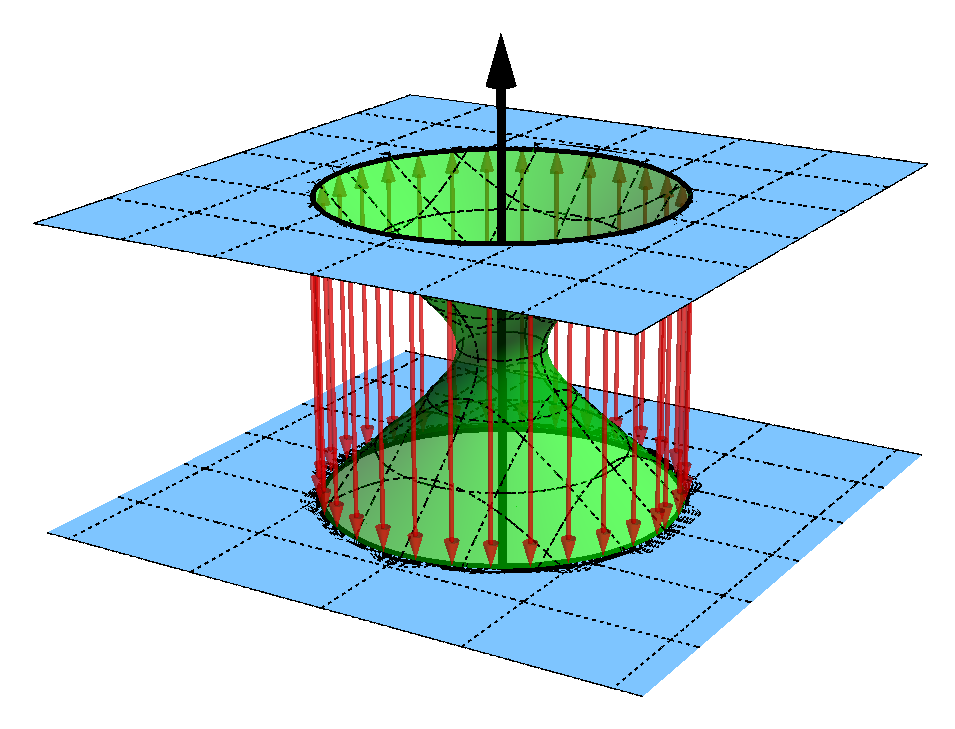
\includegraphics[width=.9\textwidth]{img/Chapter2/Identification.png}}
 \end{center}
 \caption{Pictoric image showing the identification process between the $x^2+y^2<a^2$ disks. The red arrows indicate that the two disk are glued together (not the rings) and there is no ``space'' between the two planes in this representation. The blue planes represent the $z=0$ planes in the $r>0$ and $r<0$ spaces. The green surface only serves to show the wormhole product of the identification but as the two disks are glued together, this surface does not exist in reality. Notice that in this representation the space between the two planes does not exist and therefore there is only displayed the $z>0$ semi-space of the upper copy of $\mathbb{R}^3$ and the $z<0$ semi-space of the lower copy of $\mathbb{R}^3$. The other semi-space are not in the picture as we would need another one to display them. We remark that as the green surface does not exist, topological properties cannot be derived from it. Moreover, the topology of the identification is trivial. }
 \label{fig:Identification}
\end{figure}  
It was first noticed by Brandon Carter \cite{carter1968global} that the Kerr spacetime can be extended beyond the previous description. This extension takes its origin in the fact that the Kerr metric in \gls{BL} coordinates is no singular at $r=0$ and therefore the variation range of this coordinate (initially $r\in(0,\infty)$) can be extended to $r\in(-\infty,\infty)$. This is due to the fact that the singularity is not a point but a ring. This identification is very easy to perform in \gls{KS} coordinates. First of all notice that if we restrict the values of the function $r=r(x,y,z)\in(0,\infty)$, then a geodesic that is defined along the $z$ axis ($x=y=0$) starting from the positive branch ($z>0$) will reach the disk inside the singular ring (located at $z=0,x^2+y^2<a^2$) with no problems because the inner disk is not singular, but there is still problems. For the $z>0$ axis the definition of the function $r$ that follows from \cref{eq:rdefinition} (with positive sign) is $r(x,y,z)=z$ and when the geodesic reaches the inner disk and passes through it, the definition of the function $r$ must change to $r(x,y,z)=-z$ as now $z<0$ and the function $r$ must remain positive. This change of sign in the function $r$ leads to a discontinuous definition as well as  to discontinuous curvature invariants  (like $R^{\alpha \beta \gamma \delta} R_{\alpha \beta \gamma \delta}$ (where $R^{\alpha}_{\beta \gamma \delta}$is the Riemann tensor). To remove this singularity we must extend the variation range of the function $r$ to $r(x,y,z)\in(-\infty,\infty)$ which leads to a identification between two copies of the Kerr spacetime.

\begin{proposition}
 The Kerr spacetime once the function $r(x,y,z)$ is extended to $r\in(-\infty,\infty)$ is foliated by the leafs 
 \begin{equation}
  \mathcal{M} = \frac{\mathbb{R}_+^3 \cup  \mathbb{R}_-^3}{\sim}
 \end{equation}
where in each leaf the time coordinate has a different value (which defines the foliation), $\mathcal{M}$ denotes the final \gls{MAE} manifold, $\mathbb{R}_+^3$ and $\mathbb{R}_-^3$ denotes two copies of $\mathbb{R}^3$ and $\sim$ is the equivalence relation given by
\begin{align}
 &p_1=(x_1,y_1,z_1) \in \mathbb{R}_+^3 \nonumber, \\
 &p_2=(x_2,y_2,z_2) \in \mathbb{R}_-^3 \nonumber, \\
 &p_1 \sim p_2 \longleftrightarrow \{ x_1=x_2, y_1=y_2 ,z_1=z_2=0, x_i^2+y_i^2<a^2 \}
\end{align}
The tangent planes are identified in the following way
\begin{align}
 &v_1 \in T_p\mathbb{R}_+^3,\quad \quad p \in x_1^2+y_1^2<a^2, z=0\\
 &v_2 \in T_p\mathbb{R}_-^3,\quad \quad p \in x_1^2+y_1^2<a^2, z=0\\
 &v_1 \sim v_2 \longleftrightarrow v_1^\alpha = v_2^\alpha.
\end{align}
The function $r(x,y,z)$ after de identification takes the form
\begin{align}
  r(x,y,z)&=\lambda \frac{\sqrt{\sqrt{\left(a^2-x^2-y^2-z^2\right)^2+4 a^2 z^2}-a^2+x^2+y^2+z^2}}{\sqrt{2}}\\
 \end{align}
 with $\lambda=1$ for $\mathbb{R}_+^3$ and $\lambda=-1$ for $\mathbb{R}_-^3$.
\end{proposition}
\begin{Proof}
 The implicit definition of the function $r$ in \gls{KS} coordinates given by \cref{eq:rdefinition} reads
 \begin{equation}\label{eq:rrelationident}
  r^2 \left(a^2+r^2\right)=z^2 \left(a^2+r^2\right)+r^2 \left(x^2+y^2\right).
 \end{equation}
 This equation have four solutions, two of them always real and the other two always imaginary (they are complex conjugate). The two real solutions are
 \begin{align}
  r(x,y,z)&=\frac{\sqrt{\sqrt{\left(a^2-x^2-y^2-z^2\right)^2+4 a^2 z^2}-a^2+x^2+y^2+z^2}}{\sqrt{2}}\\
  r(x,y,z)&=-\frac{\sqrt{\sqrt{\left(a^2-x^2-y^2-z^2\right)^2+4 a^2 z^2}-a^2+x^2+y^2+z^2}}{\sqrt{2}}
 \end{align}
  \begin{figure}   
\begin{center}
 \centerline{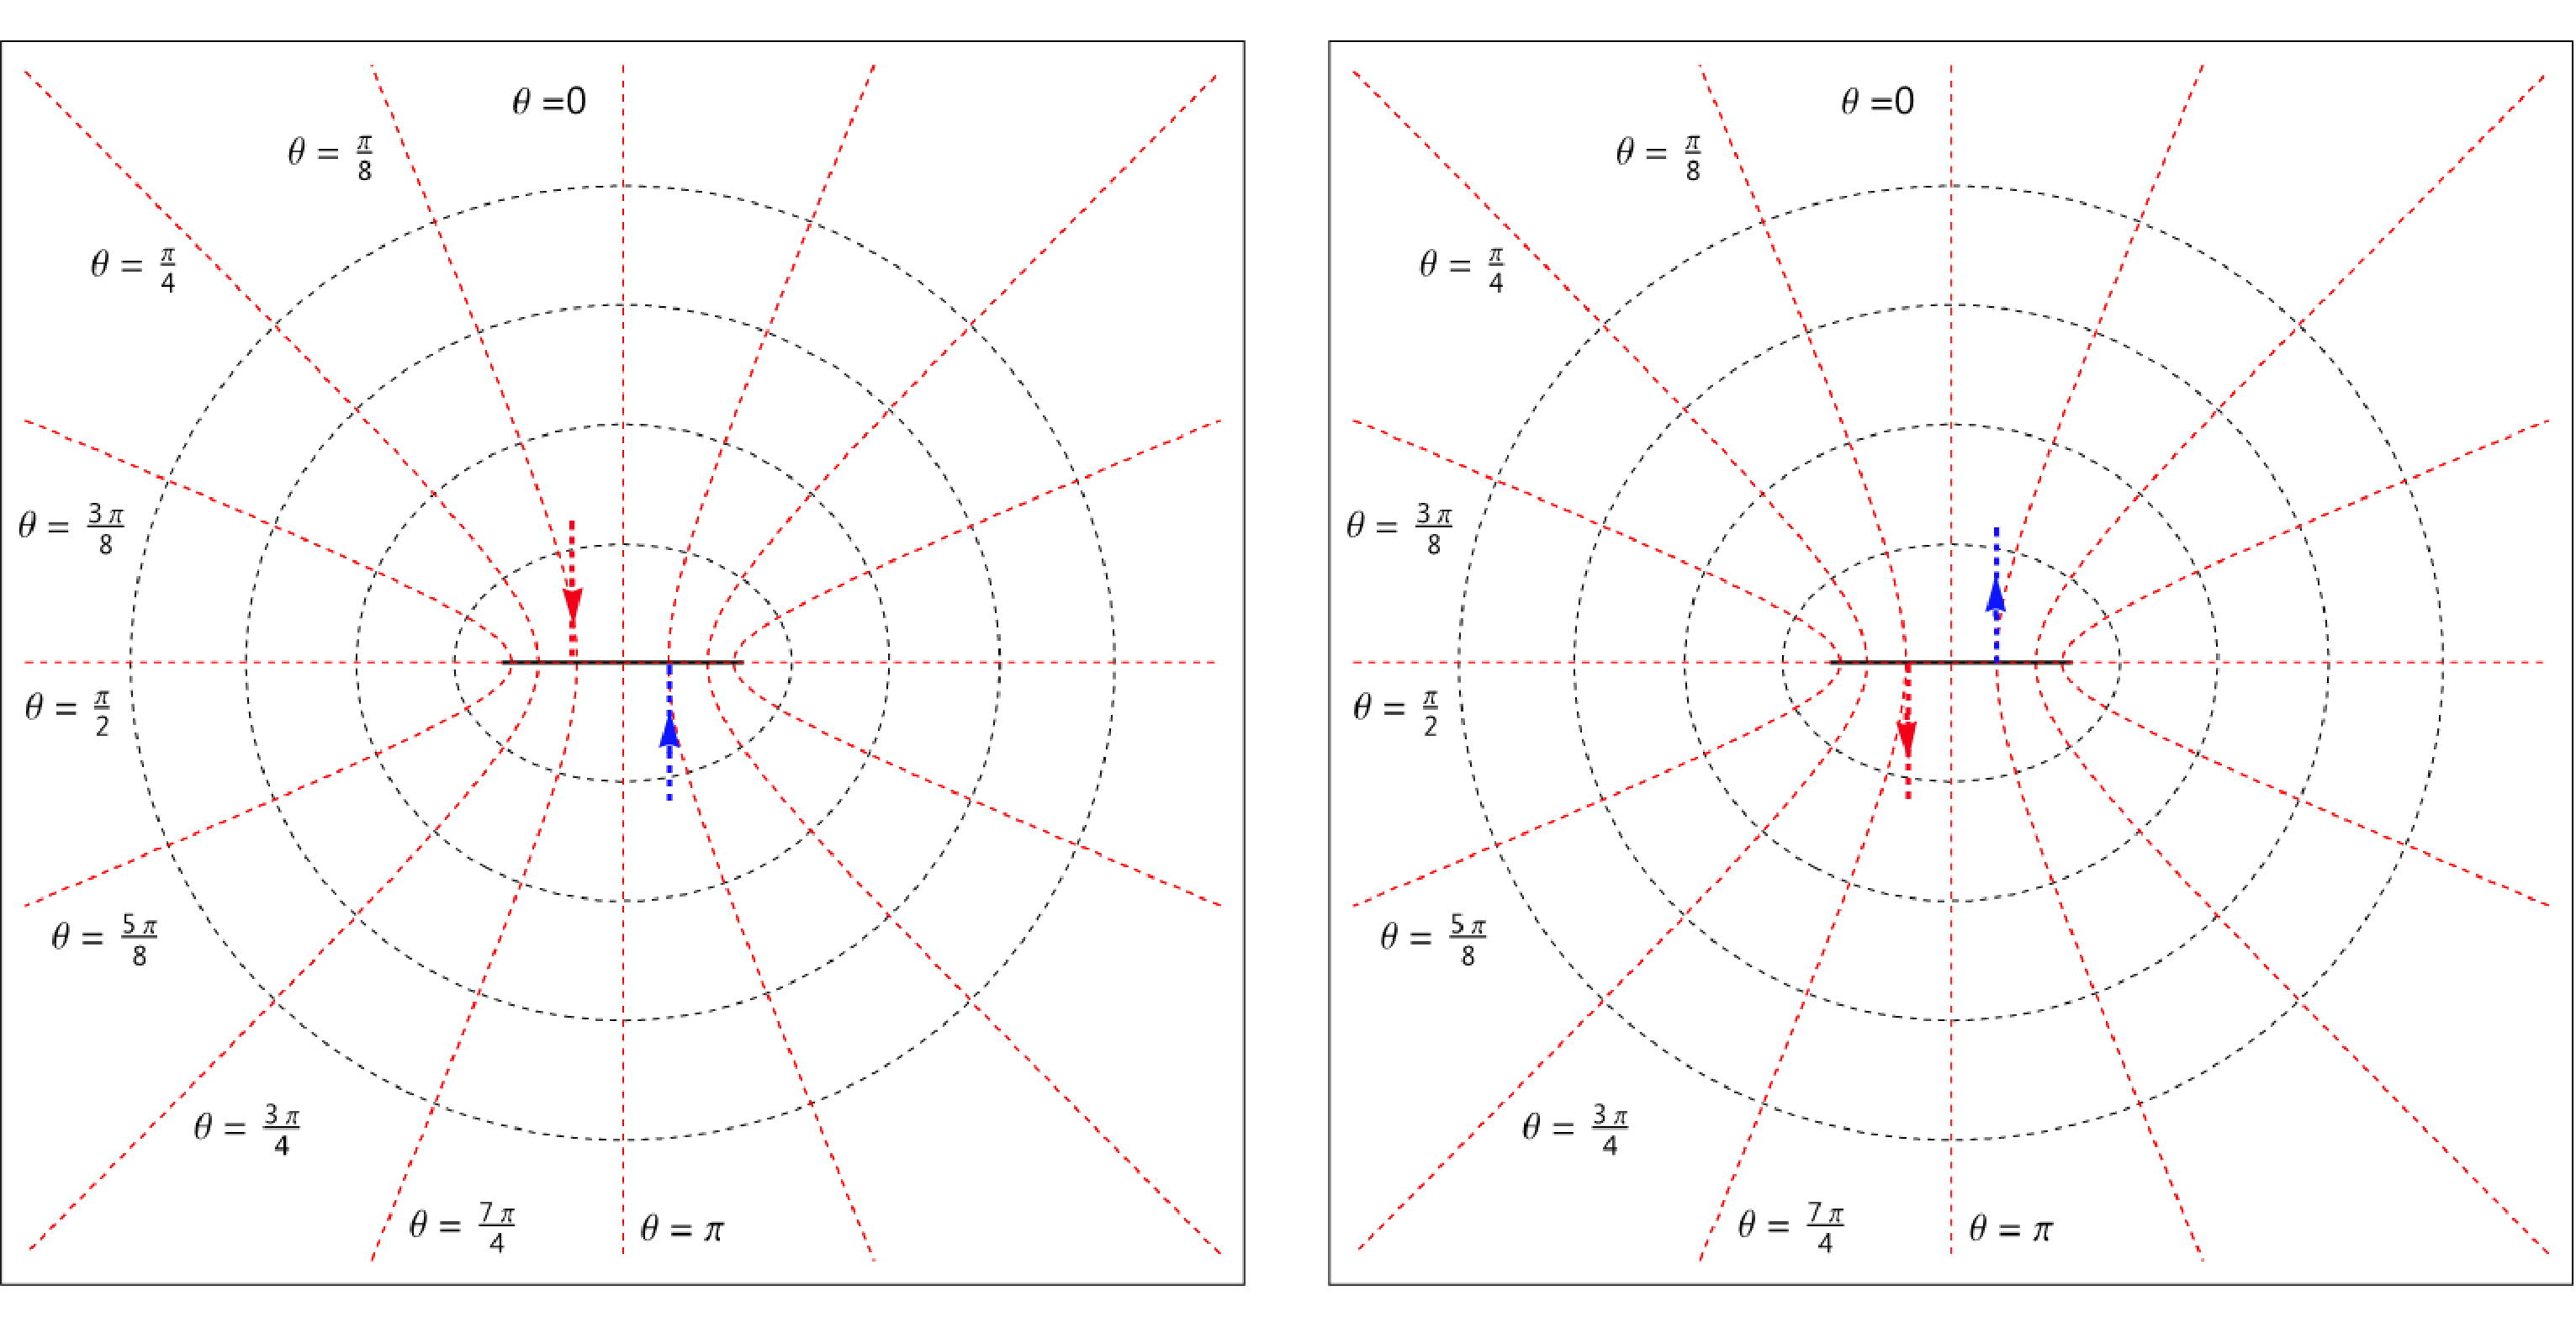
\includegraphics[width=\textwidth]{img/Chapter2/Idetification2.pdf}}
 \end{center}
 \caption{Side view of the spaces $\mathbb{R}_+^3$ (left image) and $\mathbb{R}_+^3$ (right image). The red dotted lines represent the surfaces with $\theta=const.$ while the black dotted lines represent the $r=const.$ surfaces.The singular ring is the thick black line in the middle. The arrows show how the identification works: A geodesic that follows the red arrow in the left image emerges in the right image following the red arrow and equivalently for the blue arrow. Once in the right image the situation becomes the same as it started. Note that a geodesic following one arrow can surround the ring and pass through the disk as the other arrow. As the green surface does not exist, the topological implications of its shape are inexistent, as the identification has trivial topology. }
 \label{fig:Identification2}
\end{figure} 
This is the reason that for each set of \gls{KS} coordinates there are two different values of $r(x,y,z)$. Therefore we have two different copies of the Kerr spacetime described by the metric \cref{eq:metricinKS} with different sign in the definition of the function $r(x,y,z)$. Let's name this copies $\mathbb{R}_+^3$ and $\mathbb{R}_-^3$. When we perform the similarity relation given by \begin{align}
 &p_1=(x_1,y_1,z_1) \in \mathbb{R}_+^3 \nonumber, \\
 &p_2=(x_2,y_2,z_2) \in \mathbb{R}_-^3 \nonumber, \\
 &p_1 \sim p_2 \longleftrightarrow \{ x_1=x_2, y_1=y_2 ,z_1=z_2=0, x_i^2+y_i^2<a^2 \}
\end{align}
we are constructing a topological manifold product of gluing the two disks together. In order to construct a differential manifold, we must say how we identify the tangent planes. They are under the following similarity relation:
\begin{align}
 &v_1 \in T_p\mathbb{R}_+^3,\quad \quad p \in x_1^2+y_1^2<a^2, z=0\\
 &v_2 \in T_p\mathbb{R}_-^3,\quad \quad p \in x_1^2+y_1^2<a^2, z=0\\
 &v_1 \sim v_2 \longleftrightarrow v_1^\alpha = v_2^\alpha.
\end{align}
Under this identification of the disks and the tangent planes, we are finally identifying the top the disk $x_1^2+y_1^2<a^2$,$z_1=0$ with the bottom of the disk $x_2^2+y_2^2<a^2$,$z_2=0$ and vice versa as is displayed in \vref{fig:Identification,fig:Identification2}. After the identification is complete, the definition of the function $r(x,y,z)$ becomes
\begin{align}\label{eq:rdefinitiondef}
  r(x,y,z)&=\lambda \frac{\sqrt{\sqrt{\left(a^2-x^2-y^2-z^2\right)^2+4 a^2 z^2}-a^2+x^2+y^2+z^2}}{\sqrt{2}}\\
 \end{align}
 with $\lambda=1$ for $\mathbb{R}_+^3$ and $\lambda=-1$ for $\mathbb{R}_-^3$. As the function r becomes $r(x,y,z)=0$ at the disk, we have a continuous and at least $C^2$ definition and therefore the curvature scalars are continuous. We must proof that this definition for the function $r(x,y,z)$ is also analytic. To achieve this, write for points near the inner disk ($x^2+y^2<a^2$ and $z\sim 0$)
 \begin{equation}
  r(x,y,z)=z \sqrt{f(x,y,z)}
 \end{equation}
where $f(x,y,z) : \mathbb{R}^3 \to \mathbb{R}^+$ is a everywhere positive function. Under this ansatz we can rewrite \cref{eq:rrelationident} as
\begin{equation}
 f(x,y,z) \left(z^2 f(x,y,z)+a^2-x^2-y^2-z^2\right)-a^2=0
\end{equation}
which leads to
\begin{equation}
  f(x,y,z)=\frac{\pm \sqrt{\left(-a^2+x^2+y^2+z^2\right)^2+4 a^2 z^2}-a^2+x^2+y^2+z^2}{2 z^2}
\end{equation}
to obtain a positive function we must chose the $+$ in the square root. This function satisfies that
\begin{equation}
 \lim_{z\to0}{f(x,y,z)}=\frac{-a^2}{-a^2+x^2+y^2}
\end{equation}
The function $f(x,y,z)$ is a analytic function because it is the result of composing analytic functions. As the function $z$ under the identification is continuous and analytic, we conclude that the function $r(x,y,z)$ is continuous because is the product of analytic functions. This is also because
\begin{equation}
 \lim_{z \to 0}{ z \sqrt{f(x,y,z)}}|_{x^2+y^2<a^2}=0
\end{equation}
As now the manifold is formed under a identification that leads to continuous and smooth functions and curvature scalars, we have removed the ``singularity'' across the disk. Of course, this corresponds only to the spatial part of the Kerr spacetime, i.e each foil of the whole foliation, where each foil has a different value of the time coordinate $t$.
\end{Proof} 

With this identification of the inner disk, a geodesic that falls through the $z>0$ branch of the $z$-axis with $r>0$ ($\mathbb{R}_+^3$ copy), reach the top of the inner disk at $x^2+y^2<a^2$,$z=0$ and emerges on the bottom of the inner disk of the space with $r<0$ ($\mathbb{R}_-^3$ copy). At this point, the geodesic can go to the asymptotically flat limit $r\to -\infty$. Is important to note that in the $\mathbb{R}_-^3$ copy, there are no horizons as the singularity equation $\Delta(r)=0$ only gives positive solutions for the horizons. 

As the geodesics are not necessarily defined on the $z$-axis, to fully understand this part of the Kerr \gls{MAE}, we must think in the spacetime as two complete and independent copies of $\mathbb{R}^3$. Imagine that in the two copies there is a disk inside the singular ring. If the identification is not yet done, if we travel across this disk nothing happens, i.e. if a geodesic goes from under the disk it will emerge above the disk and vice versa. This is obvious because we are only passing through a disk in a ``regular space''. Imagine now that after the identification is done, the behavior of the geodesic is the same (in the sense that if you pass through the disk from underneath you will emerge from the top and if you go across the disk from the top you will emerge from the bottom) but when you pass across the disk, you emerge in another space (another copy of $\mathbb{R}^3$) in the same way (top to bottom and bottom to top). Each copy is complete in the sense that have everything that the other copy have. Therefore, there are two different $z$-axis (one in each copy), two different singular rings (but only one disk because the identification is between the disks and no between the singular rings), two different asymptotically flat ends of the spacetime... The only thing that is not analogous between the two copies is that in $\mathbb{R}_-^3$ there is no horizons and the only singular surface is the singular ring, as was noticed previously.

Notice also that the \gls{MAE} of a geodesic that is imposed to move along the $z$-axis is formed by two disjoint parts. This is because if we consider a geodesic falling along the $z$-axis with $z>0$ in $\mathbb{R}_+$ when it reaches the inner disk, it emerges in $\mathbb{R}_-$ with $z<0$. As the geodesic is imposed to move along the axis, it cannot surround the ring and access the $z>0$ branch of $\mathbb{R}_-$ so this geodesic is forced to move in the space $\mathcal{Z}_1=\mathbb{R}_+|_{z>0} \cup \mathbb{R}_-|_{z<0}$. Similarly a geodesic that falls along the  $z$-axis with $z<0$ is forced to move in the space $\mathcal{Z}_2=\mathbb{R}_+|_{z<0} \cup \mathbb{R}_-|_{z>0}$. Indeed, the definition of the function $r(x,y,z)$ for a geodesic that falls along the $z$-axis ($x=y=0$) becomes
\begin{align}
 r(z,0,0)= \lambda z
\end{align}
with $\lambda=1$ for the space $\mathcal{Z}_1$ and $\lambda=-1$ for the space $\mathcal{Z}_2$.

 
\FloatBarrier
\section{Kerr-Schild patches}
  \begin{figure}[hpt!] 
\begin{center}
 \centerline{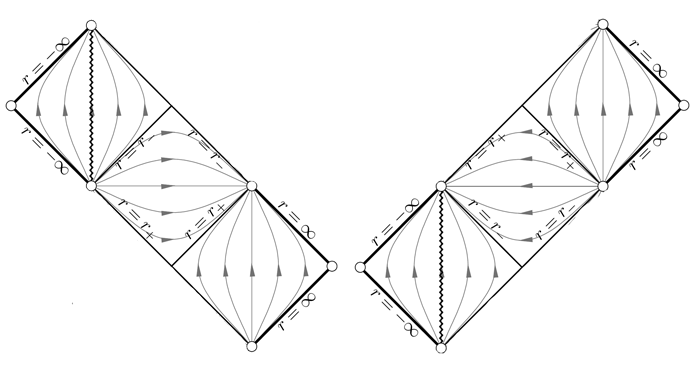
\includegraphics[width=.8\textwidth]{img/Chapter2/KerrSchild.png}}
 \end{center}
 \caption{The figure on the left shows the ingoing Kerr-Schild patch ($\sigma=-1$) while the figure on the right shows the outgoing Kerr-Schild patch ($\sigma=1$).}
 \label{fig:PenroseKS}
\end{figure} 
Actually the \gls{MAE} of the Kerr spacetime is much larger than the ring identification. We are going to study which part of the known maximal extension of the spacetime is covered by each \gls{KS} patch and how they are assembled. To do this we must know how the \gls{KS} time coordinate is related to the \gls{BL} time coordinate. From \vref{eq:Kerrcoordtrans1,eq:timeeq2} we can relate the \gls{KS} coordinate $t$ to the \gls{BL} analogue $\bar{t}$:
\begin{equation}
 d\bar{t}=dt+\sigma \left(\frac{r^2+a^2}{\Delta}-1\right).
\end{equation}
A direct integration for constant-$t$ trajectories gives
  \begin{equation}
 \bar{t}(r)=M \sigma  \left(\log \left(a^2-2 M r+r^2\right)+\frac{2 M \tan^{-1}\left(\frac{r-M}{\sqrt{(a-M) (a+M)}}\right)}{\sqrt{(a-M) (a+M)}}\right).
\end{equation}
The outer horizon is located at $r_+=M+\sqrt{\left(M^2-a^2\right)}$ and we can evaluate the function $\bar{t}(r)$ as it reaches the outer horizon, which gives that
\begin{align}
 \lim_{r \to r_+}{ \bar{t}(r)}|_{t=const.} &= - \sigma \infty,\\
 \lim_{r \to \infty}{ \bar{t}(r)}|_{t=const.} &=  \sigma \infty.
\end{align}
  \begin{figure}[htp!]
\begin{center}
 \centerline{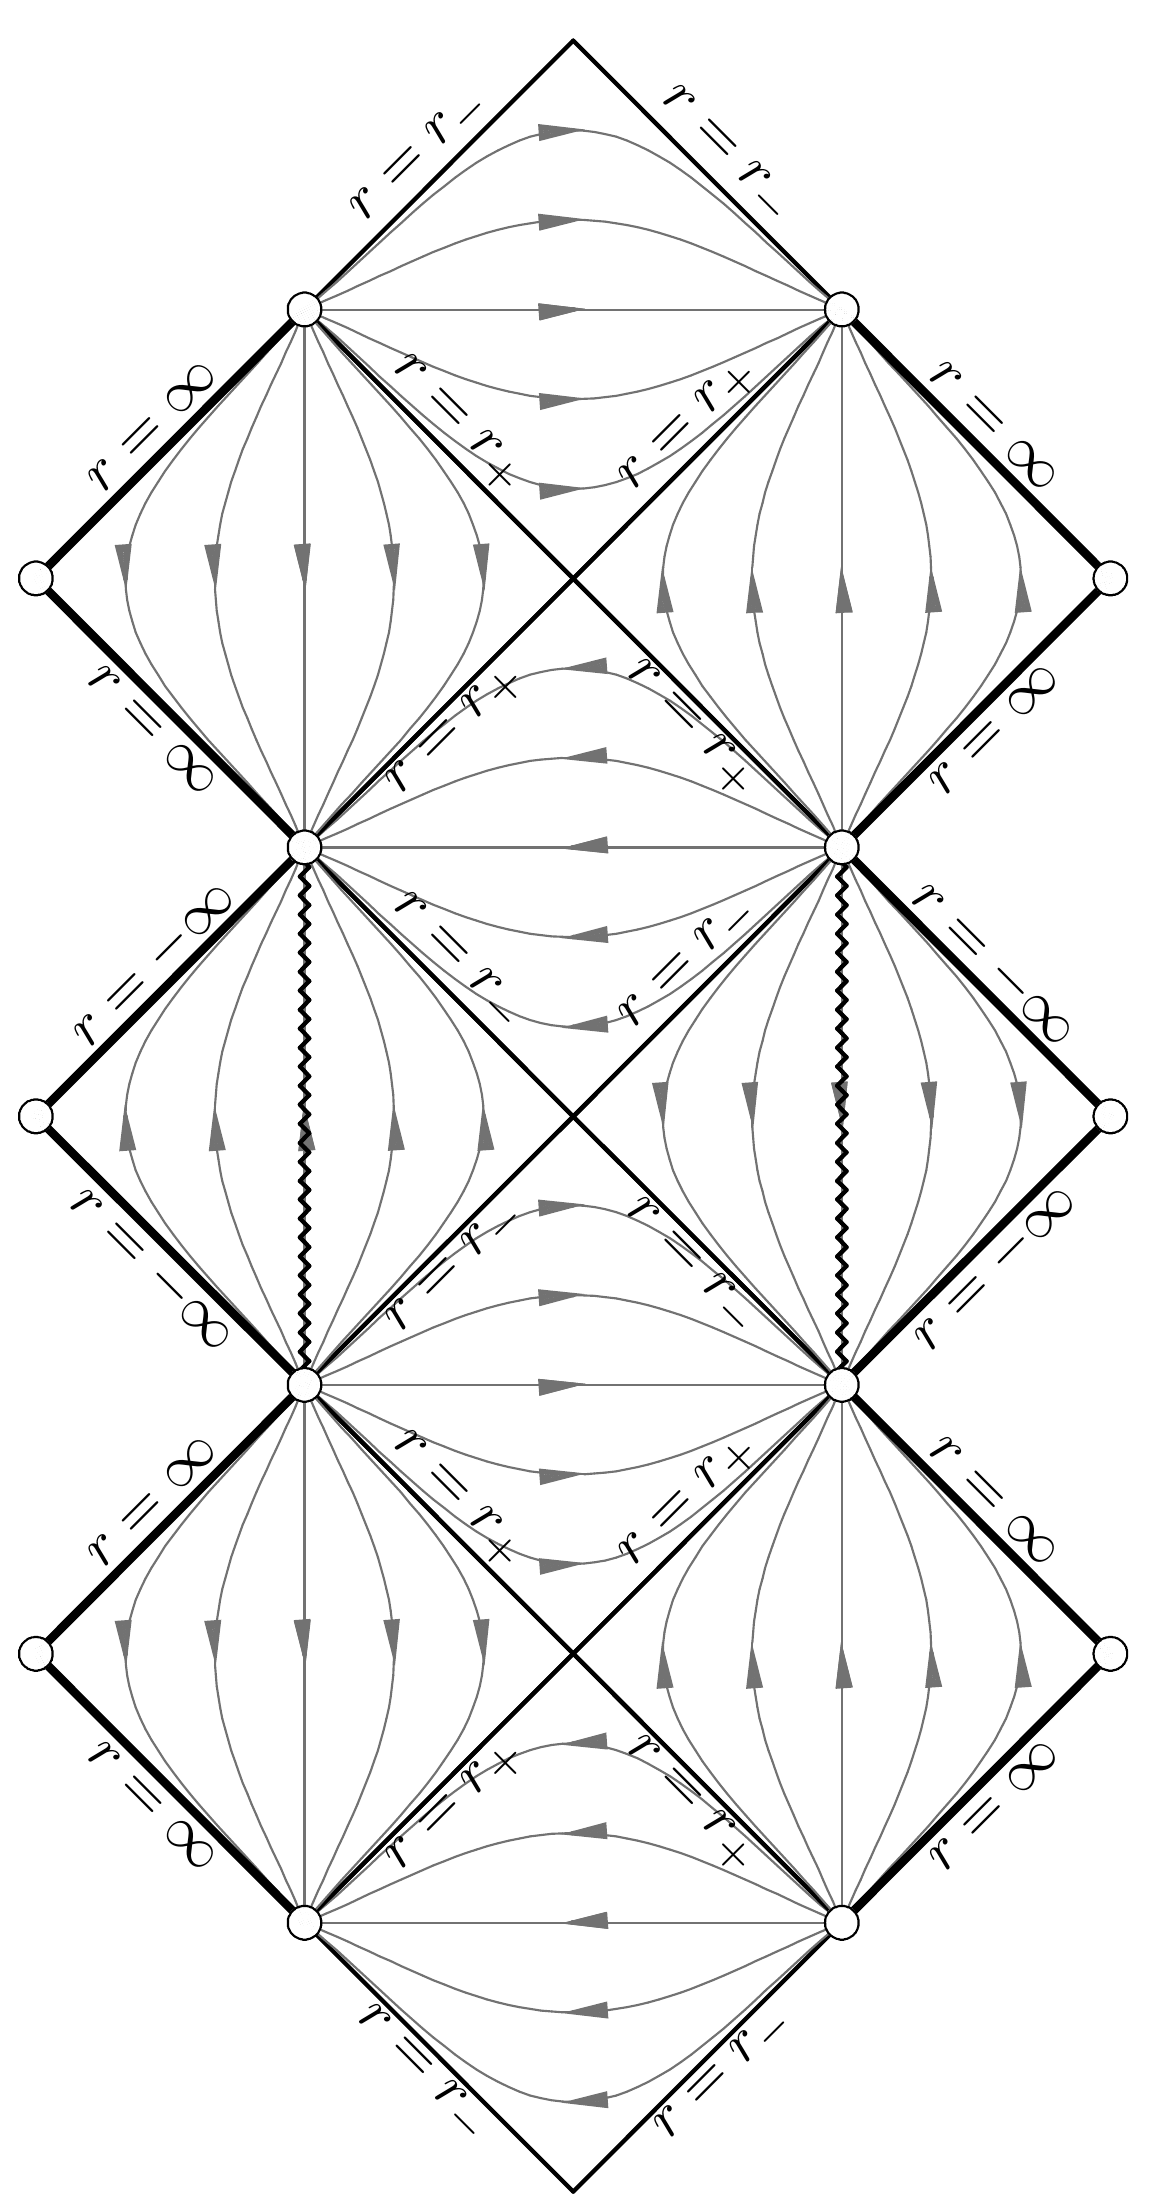
\includegraphics[width=.4\textwidth]{img/Chapter2/Diagrama.png}}
 \end{center}
 \caption{\gls{PC} diagram of the Kerr spacetime along the axis of symmetry for simplicity. The \gls{PC} diagrams are conformal compactifiactions of the spacetime that help to understand the causal structure of the whole manifold. The diagram is constructed to maintain the light cones as straight lines at $\frac{\pi}{2}$ \textit{rad}. For more information and resources to understand \gls{PC} diagrams see \cite{o1995geometry,hawking1973large}.}
 \label{fig:Penrose}
\end{figure} 
Therefore the Kerr-Schild patch with $\sigma=-1$ approaches $r \to r_+$ with $\bar{t} \to \infty$ and comes from $r=\infty$ in the past ( $\bar t=-\infty$ ) and the Kerr-Schild patch  with $\sigma=1$ approaches $r=\infty$ with $\bar{t} \to \infty$ and comes from $r \to r_+$  in the past ( $\bar t=-\infty$ ). We will assign (as is usually done in the \gls{SW} case) the denomination  \textit{Black hole} to the \gls{KS} patch with $\sigma=-1$ and \textit{White hole} to the \gls{KS} patch with $\sigma=1$. Of course, in \gls{KS} coordinates, the geodesic flow does not stop at $r_+$ and can be extended over $r_-$ until reaches $r=0$ for both values of $\sigma$. This two patches can be glued together an indefinitely number of times, allowing the geodesic flow to pass over $r_+$ and $r_-$ as many times as needed. A in-depth study of the geodesic completeness (see chapter 3 of \cite{o1995geometry}) reveal that the basic structure of the maximal extension is in reality formed by four basic patches (two of them isometric to the other two) as one can visualize in the Penrose carter diagram of \cref{fig:Penrose}. The two basic patches of the left are isometric to the two basic patches of the right (these two basic patches are the ones that we have studied), and this group is glued together and infinite number of times conforming the Penrose Carter diagram. The whole \gls{MAE} of the Kerr spacetime is not globally hyperbolic and also, if we can connect two points in the spacetime with a causal curve is not necessary true that there is a geodesic that connect this two points. Despite the \gls{MAE} is not globally hyperbolic, the two \gls{KS} patches are globally hyperbolic and therefore it is true that if we find a causal curve connecting two points, exists a geodesic that connect the same points. This is quite useful to think in the different geodesic trajectories that we are going to describe in the next chapters. As a geodesic can be extended across the \gls{PC} diagram, it can travel infinitely across the \gls{KS} regions and escape to one of the asymptotically flat regions in $r=\infty$, end in the ring singularity or even pass through one of the inner disks (one of the infinite disk in the middle of the singular rings) and cross to one of the $\mathbb{R}_-^3$ copy of the spacetime. As we can see, the geodesic behavior in the whole spacetime is very complicated even if we restrict the movement to the $z$-axis. But as we will see in the next chapters, we are going to develop a method that allows us to describe all the complicate geodesic trajectories in one simple and 2D phase space where all possible geodesics will be displayed. 

\section{Causality violations}
\begin{figure}
\begin{center}
 \centerline{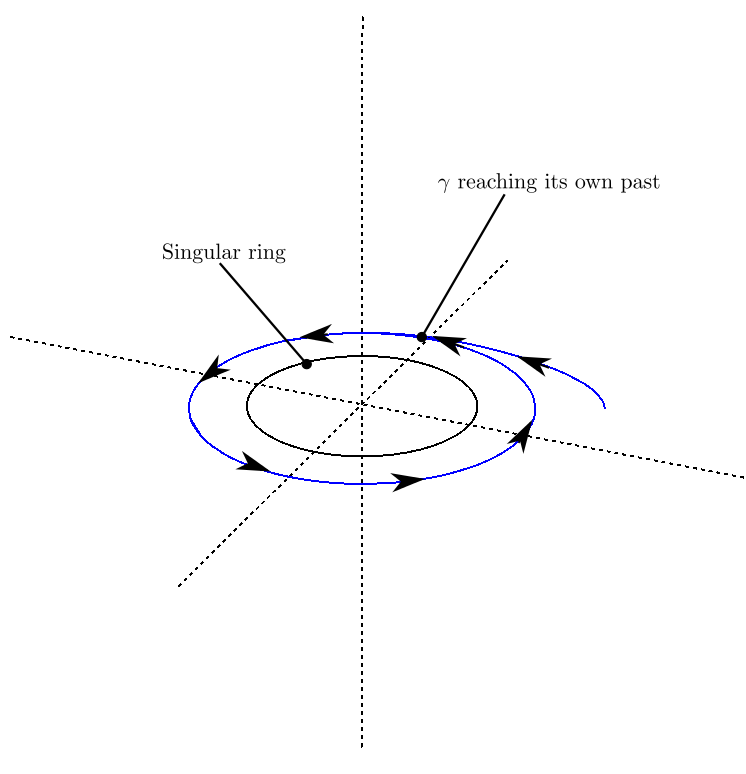
\includegraphics[width=.75\textwidth]{img/Chapter2/causal.png}}
 \end{center}
 \vspace{-1cm}
 \caption{The curve $\gamma$ as it reaches its own past.}
 \label{fig:pastgamm}
\end{figure} 
We have seen that in the region $\mathbb{R}_{-}^3$ the value of the coordinate $r$ is bounded in the interval $[-\infty,0]$. We are going to see that this lead to causality violations. This causality violations are closed causal curves that can correspond to physical observers (timelike curves with $u^\alpha u_\alpha<0$, where $u^\alpha$ is the tangent vector), which lead to time travel as the curve reach his own past for finite value of the propper time. This is easier to show in \gls{BL} coordinates. Let us consider a timelike curve $\gamma$ consisting a circle in the equatorial plane outside the singular ring in the space $\mathbb{R}_{-}^3$. This curve is defined as
\begin{equation}
 \gamma \equiv \quad \{ \bar{t}=const. \quad \theta=\frac{\pi}{2} \quad 0 \leq \bar{\phi} \leq 2 \pi \quad r<0\}.
\end{equation}
This curve can be the curve of an observer which stats in $\mathbb{R}_{+}^3$, crosses the two horizons, pass through the inner disk and goes around the equatorial plane just outside the singular ring. The norm of the tangent vector is
\begin{equation}
\begin{aligned}
  u^\alpha u_\alpha&=\frac{1}{r^2} \left((r^2+a^2)^2 - a^2 (r^2+a^2-2M r) \right) \nonumber \\
  &=\frac{1}{r^2}(r^4+r^2 a^2+2 M r a^2)=r^2+a^2+\frac{2 M a^2}{r}
  \end{aligned}
\end{equation}
If we set $|r|<<a,M$ (which we can do because the ring singularity is at $r=0$) we will have that $r^2+a^2+\frac{2 M a^2}{r}<0$ and the curve is a timelike curve that correspond to a physical observer. As the curve is a closed curve because is a ring, the curve reach itself in its own past. In any case, this is not a physical problem, as the space  $\mathbb{R}_{-}^3$ is beyond the even horizon and then cannot be observed (at least as long as we do not fall inside the black hole).


%************************************************
\chapter{Math Test Chapter}\label{ch:mathtest} % $\mathbb{ZNR}$
%************************************************
Ei choro aeterno antiopam mea, labitur bonorum pri no. His no decore
nemore graecis. In eos meis nominavi, liber soluta vim cu. Sea commune
suavitate interpretaris eu, vix eu libris efficiantur.

\section{Some Formulas}
Due to the statistical nature of ionisation energy loss, large
fluctuations can occur in the amount of energy deposited by a particle
traversing an absorber element\footnote{Examples taken from Walter
Schmidt's great gallery: \\
\url{http://home.vrweb.de/~was/mathfonts.html}}.  Continuous processes
such as multiple
scattering and energy loss play a relevant role in the longitudinal
and lateral development of electromagnetic and hadronic
showers, and in the case of sampling calorimeters the
measured resolution can be significantly affected by such fluctuations
in their active layers.  The description of ionisation fluctuations is
characterised by the significance parameter $\kappa$, which is
proportional to the ratio of mean energy loss to the maximum allowed
energy transfer in a single collision with an atomic electron:
\graffito{You might get unexpected results using math in chapter or
section heads. Consider the \texttt{pdfspacing} option.}
\begin{equation}
\kappa =\frac{\xi}{E_{\textrm{max}}} %\mathbb{ZNR}
\end{equation}
$E_{\textrm{max}}$ is the maximum transferable energy in a single
collision with an atomic electron.
\[
E_{\textrm{max}} =\frac{2 m_{\textrm{e}} \beta^2\gamma^2 }{1 +
2\gamma m_{\textrm{e}}/m_{\textrm{x}} + \left ( m_{\textrm{e}}
/m_{\textrm{x}}\right)^2}\ ,
\]
where $\gamma = E/m_{\textrm{x}}$, $E$ is energy and
$m_{\textrm{x}}$ the mass of the incident particle,
$\beta^2 = 1 - 1/\gamma^2$ and $m_{\textrm{e}}$ is the electron mass.
$\xi$ comes from the Rutherford scattering cross section
and is defined as:
\begin{eqnarray*} \xi  = \frac{2\pi z^2 e^4 N_{\textrm{Av}} Z \rho
\delta x}{m_{\textrm{e}} \beta^2 c^2 A} =  153.4 \frac{z^2}{\beta^2}
\frac{Z}{A}
  \rho \delta x \quad\textrm{keV},
\end{eqnarray*}
where

\begin{tabular}{ll}
$z$          & charge of the incident particle \\
$N_{\textrm{Av}}$     & Avogadro's number \\
$Z$          & atomic number of the material \\
$A$          & atomic weight of the material \\
$\rho$       & density \\
$ \delta x$  & thickness of the material \\
\end{tabular}

$\kappa$ measures the contribution of the collisions with energy
transfer close to $E_{\textrm{max}}$.  For a given absorber, $\kappa$
tends
towards large values if $\delta x$ is large and/or if $\beta$ is
small.  Likewise, $\kappa$ tends towards zero if $\delta x $ is small
and/or if $\beta$ approaches $1$.

The value of $\kappa$ distinguishes two regimes which occur in the
description of ionisation fluctuations:

\begin{enumerate}
\item A large number of collisions involving the loss of all or most
  of the incident particle energy during the traversal of an absorber.

  As the total energy transfer is composed of a multitude of small
  energy losses, we can apply the central limit theorem and describe
  the fluctuations by a Gaussian distribution.  This case is
  applicable to non-relativistic particles and is described by the
  inequality $\kappa > 10 $ (\ie, when the mean energy loss in the
  absorber is greater than the maximum energy transfer in a single
  collision).

\item Particles traversing thin counters and incident electrons under
  any conditions.

  The relevant inequalities and distributions are $ 0.01 < \kappa < 10
  $,
  Vavilov distribution, and $\kappa < 0.01 $, Landau distribution.
\end{enumerate}


\section{Various Mathematical Examples}
If $n > 2$, the identity
\[
  t[u_1,\dots,u_n] = t\bigl[t[u_1,\dots,u_{n_1}], t[u_2,\dots,u_n]
  \bigr]
\]
defines $t[u_1,\dots,u_n]$ recursively, and it can be shown that the
alternative definition
\[
  t[u_1,\dots,u_n] = t\bigl[t[u_1,u_2],\dots,t[u_{n-1},u_n]\bigr]
\]
gives the same result.  

%*****************************************
%*****************************************
%*****************************************
%*****************************************
%*****************************************

%************************************************
\chapter{The equatorial plane: The inner disk}\label{ch:ep} % $\mathbb{ZNR}$
%************************************************

Now that we understand the behavior of the geodesic movement along the axis of symmetry we will center our efforts in the movement restricted to the equatorial plane. The movement in the equatorial plane outside the horizons is well known in \gls{BL} coordinates. The fact that the metric is singular at the horizons prevent the geodesics to be extended across the horizons in this coordinate system. A complete analysis of the geodesic movement in the equatorial plane can be found in chapter 4 of \cite{o1995geometry}. The geodesic flow in the inner disk cannot be analyzed easily in \gls{BL} coordinates as the spacetime singularity is located at $r=0$ in this coordinates and therefore the ``ring`` shape cannot be analyzed in this coordinate system. The \gls{KS} coordinates are regular across all the horizons and in this system, the inner disk is well located at $x^2+y^2<a^2$ with $z=0$. Remember that this inner disk is the identification region between $\mathbb{R}_+$ and $\mathbb{R}_-$ as was previously noticed in \cref{ch:MAE}. As the geodesic behavior in the \gls{KS} coordinates in the equatorial plane is rather complicated and exceeds this work and because in the other hand, has been previously analyzed in more suitable coordinates, we are going to center our efforts in the inner disk.

\section{Hamiltonian equations of the geodesics}

We are going to discuss the geodesic equations inside the inner disk. Remember that this region is defined as $x^2+y^2<a^2$ with $z=0$. The complete understanding of the geodesic flow involves not only the knowledge of the geodesic equations but also the conditions that lead to future directed solutions. In this section we are going to derive the geodesic equations in the inner disk. 

\begin{theorem}\label{Th:ep}
 The geodesic equations for the Kerr metric restricted to the inner disk in \gls{KS} coordinates are the solution of the Hamilton equations derived from the Hamiltonian
 \begin{equation}
 H'=\frac{1}{2}  \vec{p}^{\,2}
\end{equation}
where $H=\frac{1}{2}(E^2-\mu)$ with $\mu=0$ for null geodesics, $\mu=1$ for timelike geodesics.
\end{theorem}
\begin{Proof}
Unless it is specified otherwise, $x^2+y^2<a^2$ is assumed. In the previous chapter, we derived a Hamiltonian ( see \cref{FinalgeneralH}) that describes the geodesic flow in the hole Kerr spacetime. We can adapt this Hamiltonian to the equatorial plane taking the limit $z \to 0$. This limit has to be computed carefully as we have terms involving $r(x,y,z)$ and $z$. The Hamiltonian is written as
\begin{equation}\label{Hamiltoniandisk}
H^{\prime}= \frac{1}{2}\left(E^2-\mu \right)
\frac{1}{2} \left( \vec{p}^{\,2}- \lim_{z \to 0}{(h)} \left( \vec{K} \cdot \vec{p} - E 
\hat{K} \right)^2 \right),
\end{equation} 
which is defined on the cotangent bundle of $\mathbb{R}^{3} \setminus \C$, where $\C$ represent the singular ring, $p=\left(p_x,p_y,0\right)$ $\vec{K}=\lim_{z \to 0}\left(\frac{x r(x,y,z)+a y}{r(x,y,z)^2+a^2},\frac{y r(x,y,z)-a x}{r(x,y,z)^2+a^2}, {\frac{z}{r(x,y,z)}}\right)$ and $\hat{K}=\sigma$. As we have studied before in \cref{ch:MAE}, the function $r(x,y,z)$ can be written near the inner disk as
 \begin{equation}
  r(x,y,z)=z \sqrt{f(x,y,\bar{z})},
 \end{equation}
 where $f(x,y,\bar{z})$ is a nonzero positive smooth function. Then, the limits can be written as
 \begin{align}
  &\lim_{z \to 0}{h}=  \lim_{z \to 0}{\frac{2 M r^3}{r^4+a^2 z^2}} =\lim_{z \to 0}{\frac{2 M (z \sqrt{f(x,y,\bar{z})})^3}{(z \sqrt{f(x,y,\bar{z})})^4+a^2 z^2}}\\
  &= \lim_{z \to 0}{\frac{2 M z f(x,y,\bar{z})^\frac{3}{2}}{ z^2 f(x,y,\bar{z})^2+a^2}}= 0,\\
  &\lim_{z \to 0}{h}=\frac{z}{r}=\frac{1}{\sqrt{f(x,y,\bar{z})}}
 \end{align}
The Hamiltonian becomes
\begin{equation}
 H'=\frac{1}{2}  \vec{p}^{\,2}
\end{equation}
so the solutions to the geodesic equations are
\begin{align}
 x(s)&=z_0 +{p_x}_0 s \\
 y(s)&=z_0 +{p_y}_0 s \\
 p_x(s)&={p_x}_0\\
 p_y(s)&={p_y}_0
\end{align}
where $s$ is the proper time $z(0)=z_0$ and $p_z(0)={p_z}_0$. With no difference if the geodesics are null or timelike.\end{Proof}

This result is very interesting because it tell us that the geodesic in the inner disk behaves as if the spacetime inside the singular ring were Minkowsky. This is analogous to the case in which a thin spherically symmetric shell is set as the source of the gravitational field. In this scenario and in virtue of Birkhoff's theorem \cite{birkhoff1923relativity} we will have the \gls{SW} metric outside the shell and the Minkowsky metric inside the shell. This also resembles the behavior of the electromagnetic field generated by a electrically charged thin shell, as in this case there is no field inside the shell and the field outside the shell behaves as the field generated by a punctual charge located at the center of the shell.

\section{Variation ranges and causal structure}\label{variationpe}
As we did in the previous chapter, we must now analyze the conditions that lead to future-oriented geodesics. This case is rather simple because the function $h_{z \to 0}=0$ for points inside the inner disk. 
\begin{lemma}
 If the time orientation of $(\M,g)$ is chosen so that
the null vector 
$K^\alpha=\left(-\sigma ,\frac{y}{a},-\frac{x}{a},\frac{\sqrt{a^2-x^2-y^2}}{a}\right)$
is future directed, then a geodesic with $\mu=0,1$ 
starting at a point $(t_0,x_0,y_0)$ with $x_0^2+y_0^2<a^2$ is future causal 
if and only if Carter's constant is positive for timelike geodesics and zero for null geodesics. 
\end{lemma}
\begin{Proof}
 As the function $h_{z \to 0}=0$ the metric in the inner disk becomes
 \begin{equation}
  g=\eta
 \end{equation}
 where $\eta$ is the Minkowsky metric. The 1-form $K$ of the Kerr metric becomes (after taking the limit $z \to 0$) $K=\left(-\sigma ,\frac{y}{a},-\frac{x}{a},\frac{\sqrt{a^2-x^2-y^2}}{a}\right)$ as $lim_{z \to 0} r(x,y,z)=0$ when $x^2+y^2<a^2$ and $\lim{z \to 0} \frac{z}{r(x,y,z)}=\frac{1}{\sqrt{f(x,y,\bar{z})}}=\frac{\sqrt{a^2-x^2-y^2}}{a}$. Before we can compute the conditions for future oriented geodesics notice that
 \begin{align}
  p_x&=dx(u)=\dot{x}, \label{eq:rel1} \\
  p_y&=dy(u)=\dot{y}, \label{eq:rel2} \\
  -E&=dt(u)=-\dot{t},\label{eq:rel3} \\
  L_z&= p_y x - p_x y= \dot{y} x- x \dot{y} \label{eq:rel4},
 \end{align}
 where $u=({t},\dot{x},\dot{y},0)$ is the tangent vector to the geodesics. The conditions that leads to future oriented casual (timelike and null) geodesics are $g(u_0, \sigma K |_{s=0}) <0$ or $g(u_0, \sigma K_{s=0}) =0$ which implies $u_0 = b \sigma K|_{s=0}$, with $b \geq 0$. This conditions reads
 \begin{equation}
  K_\alpha u^\alpha|_{s=0} = -a   \dot{t}_0+\sigma(\dot{y}_0 x_0-y_0 \dot{x}_0) \leq 0\\
 \end{equation}
where the equality is only when $u_0 = b \sigma K|_{s=0}$. There is still another relation that allows us to distinguish between null an timelike geodesics given by
 \begin{equation}
  -\mu = u_\alpha u^\alpha = -\dot{t}^2+\dot{x}^2+\dot{y}^2.
 \end{equation}
As $K^\alpha$ is a null vector, i.e $K^\alpha K_\alpha=0$, the condition $u_0 = b \sigma K|_{s=0}$ implies that $u_\alpha u^\alpha=\mu=0$. Using the \cref{eq:rel3,eq:rel4} we can rewrite this conditions as
\begin{align}
  &K_\alpha u^\alpha|_{s=0} \leq 0 \rightarrow -\sigma L_z+  a E = \mathcal{C}^{\frac{1}{2}} \geq 0\\
  &\frac{1}{2} \left( E^2-\mu \right) =  \frac{1}{2} \left( \dot{x}^2+\dot{y}^2 \right)
\end{align}
 where $C$ is the Carter's constant restricted to the equatorial plane that we have seen in \vref{Carterep} and the condition $\mathcal{C}^{\frac{1}{2}}=0$ occurs if
 $\mu=0$. Notice that the third equation is a direct consequence of \cref{Th:ep} because this equation can be written using \cref{eq:rel1,eq:rel2,Hamiltoniandisk} as
\begin{equation}
 \frac{1}{2}\left(E^2-\mu \right)=H^{\prime}=  \frac{1}{2} \left( \dot{x}^2+\dot{y}^2 \right)= \frac{1}{2} \vec{p}^{\,2}
\end{equation}
So, the only independent condition that lead to future casual geodesics is $\mathcal{C}>0$ ($\mu$=1) or $\mathcal{C}>0=0$ ($\mu=0$) as claimed.\end{Proof}

As we are going to see in the next section, causal geodesic with starting point at $x_0,y_0$ with $z_0=0$ and $x_0^2+y_0^2<a^2$ cannot remain in the inner disk.
\section{Stability of the inner disk}

Although the geodesic behavior of the inner disk is interesting, we are going to show that a geodesic that starts in the inner disk cannot remain in it. A heuristic argument that leads to this conclusion is that when we studied the axis of symmetry ($x=y=0$) the point $z=0$ was not a stable point, indeed, the geodesic flow go upwards the axis if $\dot{\bar{z}}_0=0$ (remember that $\bar z=\lambda z$, where $\lambda=\pm 1$). Now, we are going to extend this behavior to all geodesic that starts with $p_{\bar{z}}=0$ and $x_0^2+y_0^2<a^2$, $z=0$.
\begin{proposition}
 Only null geodesic that starts starts in the inner disk ($x_0^2+y_0^2<a^2$ and $\bar{z}=0$) with $\dot{\bar{z}}=0$ can remain in this region while timelike geodesics leaves the disk with $\ddot{\bar{z}}>0$.
\end{proposition}
\begin{Proof}Lets consider the general Hamiltonian that describes the geodesic flow in \gls{KS} coordinates along all the spacetime derived in \vref{Hamiltonkerrschild} that writes
\begin{equation}
H^{\prime} = \frac{1}{2} \left( \vec{p}^{\,2}- h \left( \vec{K} \cdot \vec{p} - E  \hat{K} \right)^2 \right),
\end{equation} 
defined on the cotangent bundle of $\mathbb{R}^{3} \setminus \C$, where $\C$ represent the singular ring. Here $\hat{K}=\sigma$, $\vec{p}=(p_x,p_y,p_{\bar{z}})$ and $K=-\sigma dt + \frac{r(x dx+y dy)}{r^2+a^2} + \frac{a(x dy-y dx)}{r^2+a^2}+\frac{z dz}{r}$. The function $r(x,y,z)$ is defined for points near the inner disk as
\begin{equation}
 r(x,y,\bar{z})=\bar{z} \sqrt{f(x,y,\bar{z})}
\end{equation}
where $f(x,y,\bar{z})$ is a nonzero positive smooth function. Let's start by checking what value of $p_{\bar{z_0}}$ satisfies $\dot{\bar{z}}_0=0$. The Hamilton equation for $\dot{\bar{z}}$ evaluated at $t=0 \to \bar{z}_0=0$ implies that
\begin{equation}
\dot{\bar{z}}_0=\frac{\partial H}{\partial p_{\bar{z}}}|_{t=0 \to z=0}=p_{\bar{z_0}}.
\end{equation}
So $\dot{\bar{z}}_0=0 \rightarrow p_{\bar{z_0}}=0$. We need to calculate now $\ddot{\bar{z}}_0>0$. To achieve this we are going to calculate $\dot{\bar{z}}$ and derive this equation. Then, using the Hamilton equations for $\dot{p}_x$ , $\dot{p}_y$ and $\dot{p}_z$ we can obtain the equation for $\ddot{\bar{z}}$ as a function of $z$,$p_z$,$x$,$y$,$p_x$ y $p_y$. As we will need the derivatives of $f(x,y,\bar{z})$ we can compute these from the equation that defines $r(x,y,z)$ that is
\begin{equation}
r^2 |\vec{x}|^2=\bar{z}^2 |\vec{x}|^2+r^2 \left(x^2+y^2\right).
\end{equation}
After substituting $r= \bar{z} \sqrt{f(x,y,\bar{z})}$ and derive we can obtain
\begin{align}
 \partial_x f(x,y,\bar{z})&=-\frac{2 x f(x,y,\bar{z})}{-2 \bar{z}^2 f(x,y,\bar{z})-a^2+x^2+y^2+\bar{z}^2},\\
 \partial_y f(x,y,\bar{z})&=-\frac{2 y f(x,y,\bar{z})}{-2 \bar{z}^2 f(x,y,\bar{z})-a^2+x^2+y^2+\bar{z}^2},\\
  \partial_{\bar{z}} f(x,y,\bar{z})&=\frac{2 \bar{z} (f(x,y,\bar{z})-1) f(x,y,\bar{z})}{-2 \bar{z}^2 f(x,y,\bar{z})-a^2+x^2+y^2+\bar{z}^2}.
\end{align}
The Hamilton equation $\dot{\bar{z}}=\frac{\partial H}{\partial p_{\bar{z}}}$ reads
\begin{equation}\label{eqzeta}
\hspace{-0.1\textwidth}
 \dot{\bar{z}}=\left(p_{\bar{z}}-\frac{4 f(x,y,\bar{z}) {\bar{z}}^3 \left(\frac{p_x \left(a y+\sqrt{f(x,y,\bar{z})} x {\bar{z}}\right)}{a^2+f(x,y,\bar{z}) {\bar{z}}^2}+\frac{p_y \left(\sqrt{f(x,y,\bar{z})} y {\bar{z}}-a x\right)}{a^2+f(x,y,\bar{z}) {\bar{z}}^2}-E+\frac{p_{\bar{z}}}{\sqrt{f(x,y,\bar{z})}}\right)}{2 \left( a^2 {\bar{z}}^2+f(x,y,\bar{z})^2 {\bar{z}}^4 \right)}\right)
\end{equation}
The general form of the rest Hamilton equations is quite complicated and not very enlightening to display, and therefore we are going to display the final result. After computing $\ddot{\bar{z}}$ by deriving \cref{eqzeta}, substituting the Hamilton equation for $\dot{p}_x$ , $\dot{p}_y$ and $\dot{p}_z$, and evaluating the result at $t=0$ (which implies that $x=x_0$, $y=y_0$ ,$\bar{z}=0$, $p_x=p_{x_0}$, $p_y=p_{y_0}$,$p_{\bar{z}}=0$) we obtain that
\begin{align}
 \ddot{x}_0&=0\\
  \ddot{y}_0&=0\\
   \ddot{\bar{z}}_0&=\frac{f(x,y,\bar{z})^{3/2} (a E-\sigma L_z)^2}{a^4}=\frac{f(x,y,\bar{z})^{3/2} \mathcal{C}}{a^4}\\
\end{align}
As from \cref{variationpe} timelike geodesics starting at the inner disk must have $\mathcal{C}>0$ and therefore $\ddot{\bar{z}}_0>0$ while null geodesics can have  $\mathcal{C}=0$ and remain in the inner disk as claimed.\end{Proof}
\begin{figure}[hpt!]
\begin{center}
 \centerline{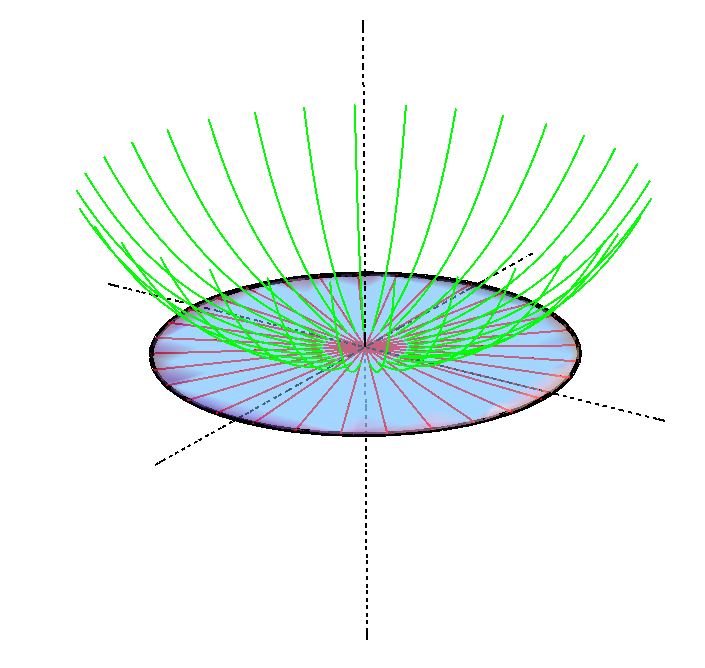
\includegraphics[width=0.75\textwidth]{img/Chapter5/Esc.png}}
 \end{center}
 \caption{The behavior of causal geodesics that start in the inner disk is depicted in this figure. The black dashed lines are the Cartesian axes, the green curves represent the causal geodesic at its first order of approximation, the red curves represent the background geodesic in the inner disk (the behavior that the geodesic would have if $\mathcal{C}=0$). The blue region represent the inner disk and the black ring represent the singular ring.}
 \label{fig:escape}
\end{figure} 

This shows that as the acceleration of the particle must be positive at the points in the inner disk, then the particle will start moving upwards $\bar{z}$ as is shows in \cref{fig:escape}. Of course, this is in perfect agreement with the results derived in \cref{ch:dinamicsys}, implying that a particle starting in $\bar{z}=0$ with $\dot{\bar{z}}=0$ will move in the direction that $\bar{z}$ increases (what we have called \textit{upwards}).

\section{A glimpse at the geodesics outside the inner disk}

As we said above, the geodesic flow outside the inner disk in the equatorial plane is hard to analyze, mostly because the causal structure is very complicated. In this section we are going to derive a energy-like equation for the geodesics in the Equatorial plane, that we are not going to analyze because it exceeds this work. The main difference between outside the ring and inside the ring is that outside the ring the function $r(x,y,z)$ is defined as
\begin{equation}\label{rinplane}
 \lim_{z \to 0} r(x,y,z)|_{x^2+y^2>a^2}= \sqrt{x^2+y^2-a^2}.
\end{equation}
and therefore the Hamiltonian \cref{Hamiltoniandisk} becomes in this case
\begin{equation}\label{Hamiltonplanoeq}
H^{\prime}= \frac{1}{2}\left(E^2-\mu \right)
\frac{1}{2} \left( \vec{p}^{\,2}- h \left( \vec{K} \cdot \vec{p} - E 
\hat{K} \right)^2 \right),
\end{equation} which is defined on the cotangent bundle of $\mathbb{R}^{3} \setminus \C$, where $\C$ represent the singular ring, $p=\left(p_x,p_y,0\right)$ $\vec{K}=\left(\frac{x r(x,y,z)+a y}{r(x,y,z)^2+a^2},\frac{y r(x,y,z)-a x}{r(x,y,z)^2+a^2},0\right)$ and $\hat{K}=\sigma$. The next theorem proofs that there exist a Energy-like equation for the geodesic movement in the equatorial plane.
\begin{theorem}
 The geodesic equations for the Kerr metric restricted to the equatorial plane outside the inner disk in \gls{KS} coordinates are the solution of the Energy-like equation
 \begin{equation}
 \frac{1}{2} \left( E^2-\mu \right) = \frac{1}{2} \left( \rho'^2 +\frac{L_z^2}{\rho^2}\right)-\frac{ M \mathcal{C}}{(\rho^2-a^2)^\frac{1}{2} \rho^2}-\frac{ \mu  M (\rho^2-a^2)^\frac{1}{2}}{\rho^2}.
 \end{equation}
where $\mathcal{C}$ is the Carter's constant, $L_z$ is the axial angular momentum, $\mu=1$ for timelike geodesics and $\mu=0$ for null geodesics and $\rho^2=r^2+a^2$.
\end{theorem}
\begin{Proof}
 The Hamiltonian \ref{Hamiltonplanoeq} reads
 \begin{equation}
  \frac{1}{2} \left( E^2-\mu \right)= H'=\frac{1}{2} \left(\vec{p}^{\,2}-\frac{h \left(E |\vec{x}|^2 +a (p_y x-p_x y)-r (p_x x+p_y y)\right)^2}{(|\vec{x}|^2)^2}\right)
 \end{equation}
 where $\vec{x}=(x,y)$. The angular momentum equation can be written from its definition ($L_z= p_y x - x p_y$) as $\vec{L_z}^2=(\vec{x} \times \vec{p})^2=\vec{x}^2 \vec{p}^{\,2}-(\vec{x} \cdot \vec{p})^2 $. We can use this relation to write the Hamiltonian as
 \begin{equation}\label{hamil2}
  H'=\frac{1}{2} \left(\frac{L_z^2+(\vec{x} \cdot \vec{p})^2}{|\vec{x}|^2}-\frac{h \left(E |\vec{x}|^2 +a L_z-r \vec{x} \cdot \vec{p}\right)^2}{|\vec{x}|^4}\right).
 \end{equation}
As from \cref{rinplane} one can derive that $r \dot{r} = \vec{x} \cdot \dot{\vec{x}}$, multiplying the Hamilton equation $\dot{\vec{x}}=\frac{\partial H}{\partial \vec{p}}$ by $\vec{x}$ we obtain that
\begin{equation}
 \vec{x} \cdot \dot{\vec{x}}=r \dot{r}=\frac{2 M \left(E |\vec{x}|^2 +a L_z\right)+\vec{x} \cdot \vec{p} (|\vec{x}|^2-2 M r)}{|\vec{x}|^2},
\end{equation}
from where we can solve for $\vec{x} \cdot \vec{p}$ and then, substituting this into the Hamiltonian of the \cref{hamil2}, which becomes
\begin{equation}
  H'= \frac{2 L_z^2 M |\vec{x}|^2+|\vec{x}|^2 \left(4 a E L_z M +2 E^2 M |\vec{x}|^2-L_z^2 r-r^3 r'^2\right)}{2 r |\vec{x}|^2 (2 M r-|\vec{x}|^2)}.
\end{equation}
As $H^{\prime}= \frac{1}{2}\left(E^2-\mu \right)$ we can write
\begin{equation}
\frac{1}{2}\left(E^2-\mu \right)=\frac{2 L_z^2 M |\vec{x}|^2+|\vec{x}|^2 \left(4 a E L_z M +2 E^2 M |\vec{x}|^2-L_z^2 r-r^3 r'^2 \right)}{2 r |\vec{x}|^2 (2 M r-|\vec{x}|^2)}.
\end{equation}
Rearranging this equation and substituting $|\vec{x}|^2=r^2+a^2$ can obtain
\begin{equation}
 E^2-\mu= r'^2+\frac{L_z^2}{r^2}-\frac{a^2 \left( E^2- \mu \right)}{r^2}-\frac{2 M \mathcal{C}}{r^3}-\frac{2 \mu  M}{r}
\end{equation}
which is not a Energy equation because it has $ E^2-\mu=2\epsilon$ (where $\epsilon$ is the Newtonian energy) in both sides. We can obtain get a new equation with the term $ E^2-\mu$ only in one side of the equation taking common factor in this term as
\begin{equation}
 \left( E^2-\mu  \right) \left( 1+\frac{a^2}{r^2} \right)= r'^2+\frac{L_z^2}{r^2}-\frac{2 M \mathcal{C}}{r^3}-\frac{2 \mu  M}{r}.
\end{equation}
Leaving alone this term in the left side the equation reads
\begin{equation}
 E^2-\mu =\left(\frac{r^2}{r^2+a^2} \right) r'^2 +\frac{L_z^2}{r^2+a^2}-\frac{2 M \mathcal{C}}{r(r^2+a^2)}-\frac{2 \mu  M r}{r^2+a^2}.
\end{equation}\label{preenergy}
which is not still a Energy-like equation because the term that goes with $ r'^2 $ is not a Kinetic-Energy term because it has the factor $\frac{r^2}{r^2+a^2} $. To finally obtain a Energy-like equation we can perform the transformation
\begin{equation}
 \rho^2=a^2+r^2
\end{equation}
as $\rho \rho ' = r r'$, then the \cref{preenergy} becomes
\begin{equation}
 \frac{1}{2} \left( E^2-\mu \right) = \frac{1}{2} \left( \rho'^2 +\frac{L_z^2}{\rho^2}\right)-\frac{ M \mathcal{C}}{(\rho^2-a^2)^\frac{1}{2} \rho^2}-\frac{ \mu  M (\rho^2-a^2)^\frac{1}{2}}{\rho^2}.
\end{equation}
\end{Proof}

First of all, notice that as the ring singularity is located at $x^2+y^2=r^2-a^2=a^2$ this implies that $r\in(0,\infty)$ and therefore $\rho \in (a,\infty)$. So the terms with $\rho^{-n}$ ($n>0$) are not divergence-terms because they are bounded by $\frac{1}{a^n} \leq \frac{1}{\rho^n}$. The true divergence-term is $(\rho^2-a^2)^{-\frac{1}{2}}$. We say that this is a Energy-like equation because it can be decomposed as
\begin{equation}
 \epsilon=\left( E^2-\mu \right) = T + V 
\end{equation}
where $T= \frac{1}{2} \left( \rho'^2 +\frac{L_z^2}{\rho^2}\right)$ is the kinetic energy in spherical-like coordinates and $V=V(\rho)=-\left( \frac{ M \mathcal{C}}{(\rho^2-a^2)^\frac{1}{2} \rho^2}+\frac{ \mu  M (\rho^2-a^2)^\frac{1}{2}}{\rho^2} \right)$ is the potential. Notice that as the Carter's constant depends on the Energy as $\mathcal{C}=(a E-\sigma L_z)^2$ this is not a true Energy equation, but can be analyzed like that if we impose this relation for the Carter's constant. Notice also that in the limit $a\to 0$ the equation becomes
\begin{equation}
 \frac{1}{2} \left( E^2-\mu \right) = \frac{1}{2} \left( \rho'^2 +\frac{L_z^2}{\rho^2}\right)-\frac{ M L_z^2}{\rho^3}-\frac{ \mu  M}{\rho}.
\end{equation}
that is the Energy equation for \gls{SW} geometry in \gls{KS} coordinates (see \cite{galindo2014mcgehee} for more information). To analyze the general Kerr Energy-like equation, we must obtain first the conditions that lead to future directed causal geodesics, but this task is quite complicated and exceeds the present work. As the ring singularity in some way regularizes the terms that diverge as $\frac{1}{\rho^n}$ (when we see the Kerr equation as an extension from the $\gls{SW}$ equation), we must deal only with the $(\rho^2-a^2)^{-\frac{1}{2}}$ divergence term. As was analyzed in \cite{galindo2014mcgehee}, once we have solved the conditions that lead to future directed casual geodesics, a interesting analysis of this equation would be based on apply the McGehee method to the phase space which derives from this equation. The Mcgehee method is a procedure that allows us to analyze the behavior of divergence dynamic systems near the singular points (and also \textit{in} the singular points). Although this is very interesting and novel, we left it for future work.

%************************************************
\chapter{Numerical resolution of the geodesics}\label{ch:nsog} % $\mathbb{ZNR}$
%************************************************

In order to understand more the general behavior of the geodesic flow in the Kerr spacetime, a numerical integration of the geodesic has been performed. The numeric code that has been used has been developed in \textit{C++} using a modified Runge-Kuta 11 method, which avoids convergence problems in different horizons. The input for this program consists in a set of initial conditions $(a,r_0,L_z,\theta_0,p_{\theta_0})$ where $a$ is the rotation parameter of the Kerr black hole, $(r_0$,$\theta_0$,$p_{\theta_0})$ are the initial values of the \gls{BL} coordinates at the starting point of the geodesic and $L_z$ is the value of the axial angular momentum. The output of this program consist in a \textit{.txt} file with the values of $(\tau_i,x_i,y_i,z_i)$ (where the index $i$ denotes the step of the numerical integration). In order to represent the trajectories the \textit{.txt} file has been import into \textit{Wolfram Mathematica}, where we have used the representation capabilities of this program to make the final plots. The legend in each plot is

\begin{itemize}
 \item The black sphere represent the outer horizon $r=r_+$. As a geodesic that cross this point cannot be seen beyond the horizon, the behavior of the geodesic flow beyond this point is not in the figures, as we want to show how a test particle will be seen from \textit{outside}.
 \item The green transparent sphere represent the outer ergosphere.
 \item The blue curve represent the geodesic path over the integration.
 \item The dashed black lines represent the $(x,y,z)$ axes.
\end{itemize}

The values of each initial condition set is included in the caption of each figure, with a brief explanation of the corresponding orbit.




\begin{figure*}
\centering
 \hspace*{-0.05\textwidth}
\begin{tabular}{cc}
\centerline{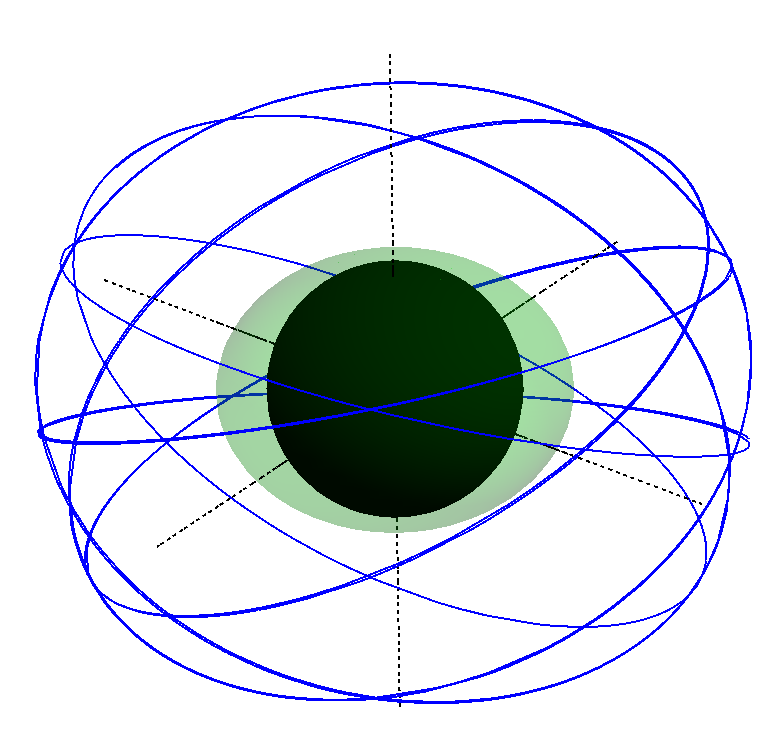
\includegraphics[width=0.7\textwidth]{img/Chapter4/ClosedOrbit.png}}
\end{tabular}
\caption{The figure shows a closed geodesic outside the outer horizon in the Kerr geometry. As is well known, closed geodesics are a very important class of orbits that provide very useful information of the spacetime and the geodesic taxonomy. In this figure, the closed orbit is not restricted to to any plane and runs across all the spacetime. }
\end{figure*}

\clearpage

\begin{figure*}
\centering
 \hspace*{-0.05\textwidth}
\begin{tabular}{cc}
\centerline{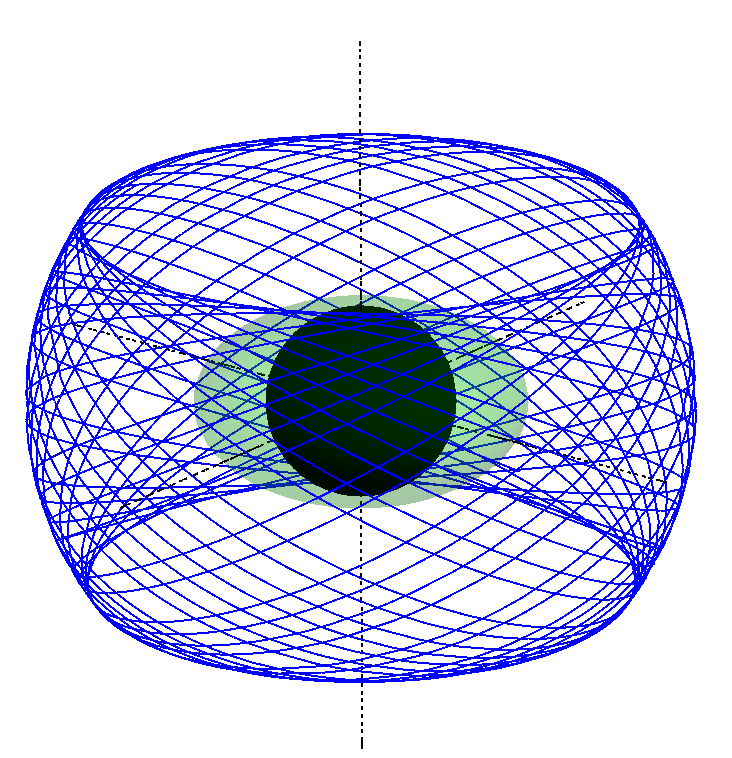
\includegraphics[width=0.7\textwidth]{img/Chapter4/Constantradius.png}}
\end{tabular}
\caption{The figure shows a geodesic with constant value of the coordinate $r$ (in \gls{BL} coordinates). This kind of motion is not as interesting as the closed orbit motion, but also provides useful information because, as we can see in the figure, this kind of geodesics are bounded between two limit circles whose height depend on the initial value of the Carter's constant. }
\end{figure*}

\clearpage

\begin{figure*}
\centering
 \hspace*{-0.05\textwidth}
\begin{tabular}{cc}
\centerline{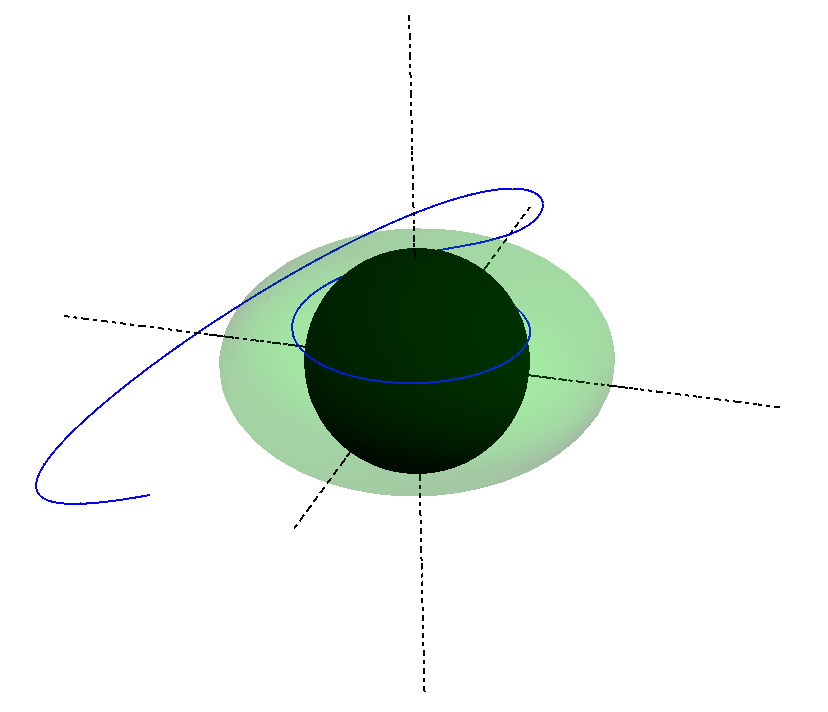
\includegraphics[width=1\textwidth]{img/Chapter4/Reversal.png}}
\end{tabular}
\caption{The figure shows what is known as the \textit{Ergosphere capture}, that is a process in which the geodesic tries to enter the ergosphere counterclockwise to the Kerr black hole rotation (in this case with its angular momentum pointing upwards) and as the properties of the Kerr geometry avoid that kind of movement, the geodesic is bend inwards and enters the ergosphere co-rotating with the Kerr black hole. Then, the geodesic is trapped in a circular co-rotating motion that ends in the outer horizon. This ergosphere capture is bounded to the equatorial plane.}
\end{figure*}

\clearpage

\begin{figure*}
\centering
 \hspace*{-0.05\textwidth}
\begin{tabular}{cc}
\centerline{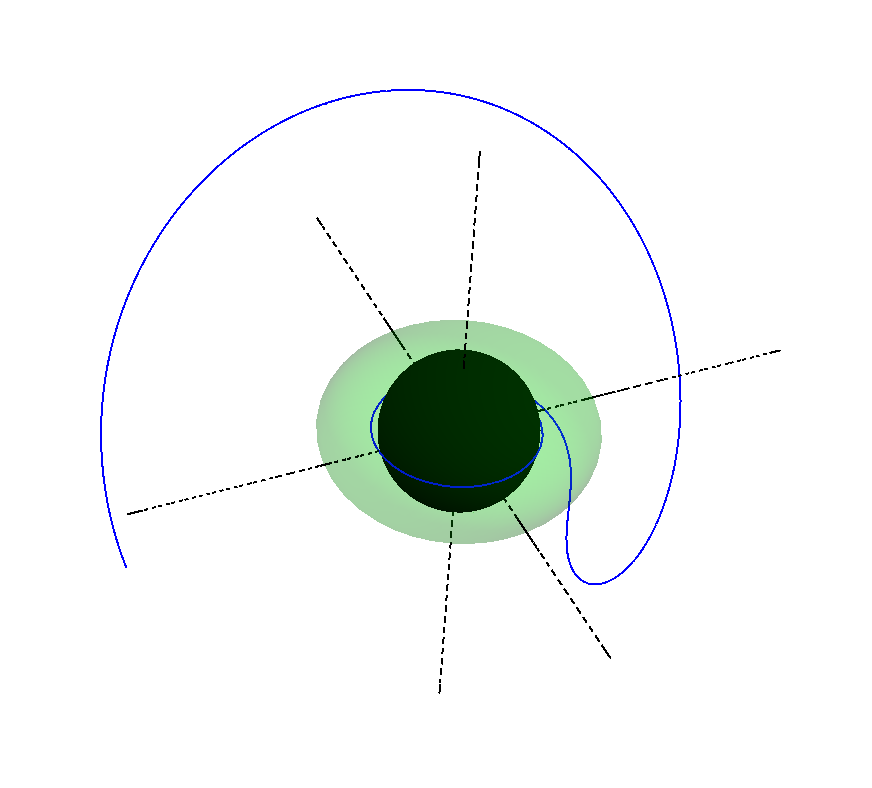
\includegraphics[width=1\textwidth]{img/Chapter4/Caputure.png}}
\end{tabular}
\caption{The figure shows another ergosphere capture but this time, the process is not bounded to a plane. As we can see in this image, the process is quite similar to the previous one, but this time the geodesic travels from the top to bottom after entering being captured by the ergosphere and bended inwards to be finally capture in a co-rotating movement that ends in the outer horizon.}
\end{figure*}


\clearpage


\begin{figure*}
\centering
\hspace*{-0.275\textwidth}
\begin{tabular}{cc}
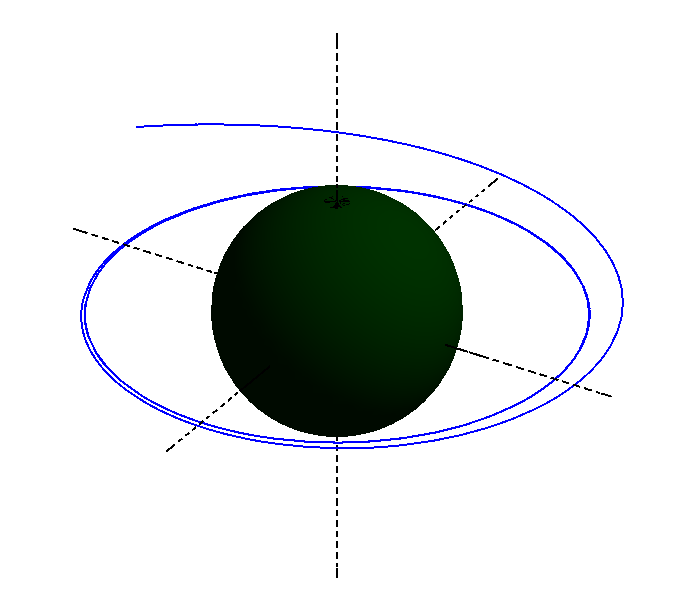
\includegraphics[width=0.6\textwidth]{img/Chapter4/ISCO1.png}&
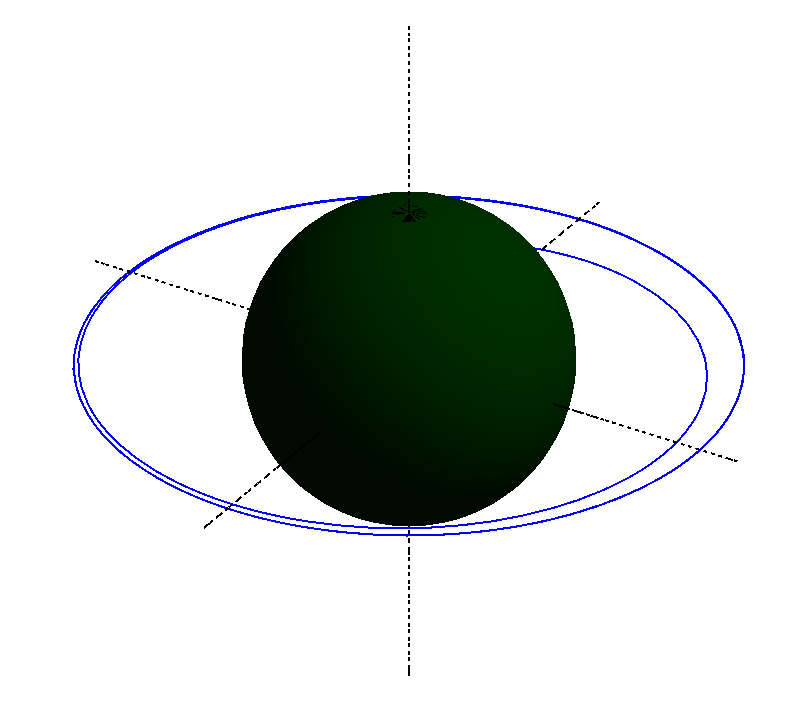
\includegraphics[width=0.6\textwidth]{img/Chapter4/ISCO2.png}\\
\end{tabular}
\caption{The two figures shows the behavior of the Innermost stable circular orbits (ISCOs). In the figure on the left, a geodesic that comes from the asymptotically flat region falls into the ISCO and remains there, while in the figure on the right, a particle that is initially at the ISCO is perturbed and trapped by the gravitational field of the black hole.}
\end{figure*}

\clearpage

\begin{figure*}
\centering
 \hspace*{-0.05\textwidth}
\centerline{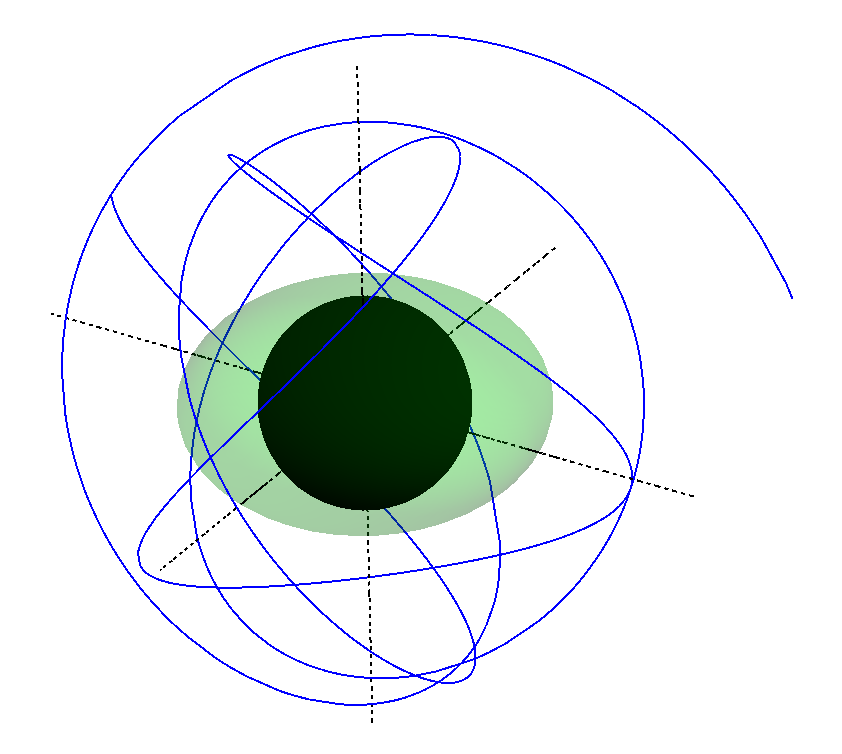
\includegraphics[width=1\textwidth]{img/Chapter4/Whirl.png}}
\caption{The figure shows what is known as the Whirl orbit. This kind of orbits may seem chaotic (and indeed they are) but they helped to understand and study the geodesic taxonomy based on the values of the Carter's constant. In this figure, the principal Whirl orbit is depicted. This kind of orbits are bounded asymptotically by the coordinate $r$ (in \gls{BL} coordinates) once they get near the ergosphere but they are not bounded by the coordinates $\theta$ and $\phi$, which gives the geodesic its characteristic behavior.}
\end{figure*}

\clearpage

\begin{figure*}
\centering
 \hspace*{-0.05\textwidth}
\centerline{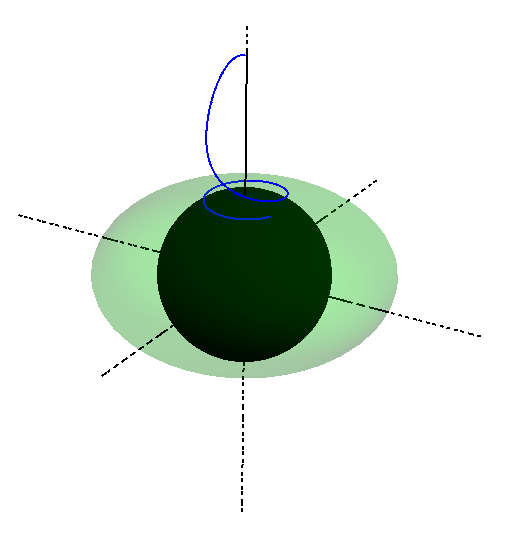
\includegraphics[width=0.75\textwidth]{img/Chapter4/ejein.png}}
\caption{The figure shows the real behavior of a geodesic trajectory that is perturbed away from the axis of symmetry. The geodesic go away from the axis and when reaches the ergosphere, the frame dragging effect starts and force the geodesic to spin co-rotating with the black hole to finally being captured by the outer horizon.}
\end{figure*}

\begin{figure*}
\centering
 \hspace*{-0.05\textwidth}
\centerline{\includegraphics[width=0.85\textwidth]{img/Chapter4/ZAMOS.png}}
\caption{The figure shows the trajectories with zero angular momentum in the Kerr spacetime. Notice how in the first stages of the movement, the trajectories are straight lines and as the geodesics approaches the black hole, they are dragged by the ergosphere and acquire the \gls{ZAMO} angular velocity before cross the outer horizon.}
\end{figure*}



% 
% \begin{figure*}
% \centering
% \hspace*{-0.1\textwidth}
% \begin{tabular}{cc}
% 
% 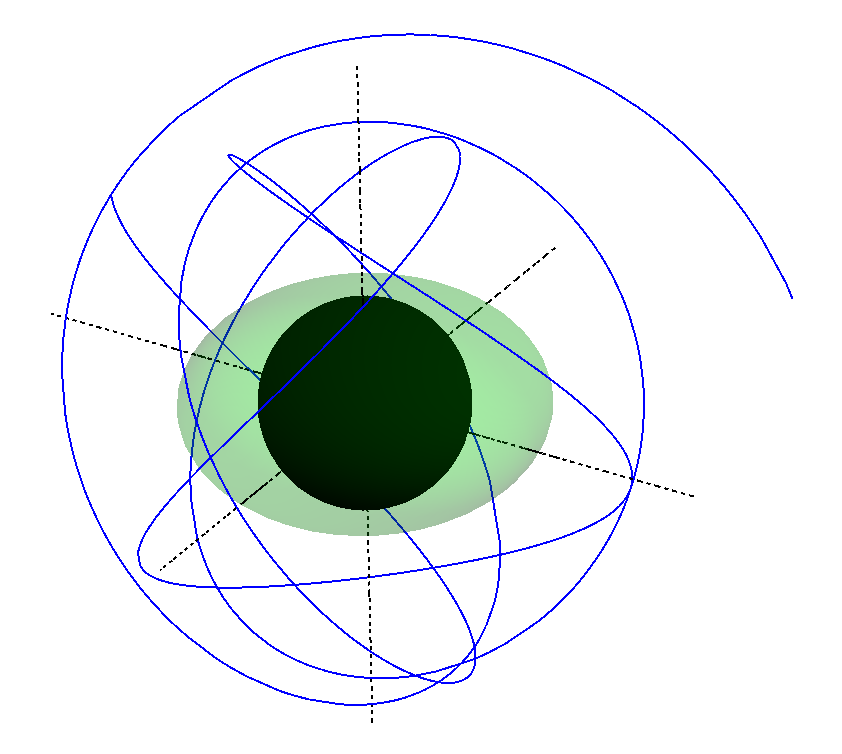
\includegraphics[width=0.5\textwidth]{img/Chapter4/Whirl.png}&
% 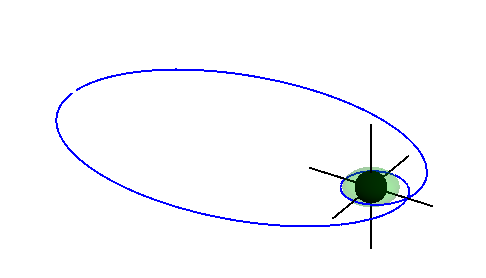
\includegraphics[width=0.5\textwidth]{img/Chapter4/Equatorial.png}\\
%
% \end{tabular}
% \end{figure*}
\part{Conclusions and comments}
%************************************************
\chapter{Conclusions}\label{ch:Concl}
%************************************************

The main result of this work is a detailed understanding of the motion
of particles in free fall in the Kerr geometry, both for massless and massive
particles. We have focused on the analysis of the axis of symmetry, the equatorial plane, and, in particular, the disk inside the singular ring of the Kerr black hole. Some of the most remarkable aspects in this work are, for example, the importance of the excluded regions, which provide the necessary topology to the physical region of the phase space to cover the whole structure of the
Penrose-Carter diagram in a single two-dimensional phase space. We have obtained completely new results on the geodesic flow in the axis of symmetry and in the inner disk from the point of view of dynamical systems, which as discussed above, is a novel approach to the problem. Some of these results are the existence of two critical points in the geodesic flow for timelike particles in the axis of symmetry, the fact that the axis of symmetry is stable, the result about the period of the lower energy orbit (which unexpectedly increases as the rotation increases) or the fact that only null geodesics that starts in the inner disk can remain in it. We have also found that the spacetime inside the singular ring behaves as the Minkowsky spacetime, analogous to the behavior of a thin, electrically charged shell, in which there is no electrical field. In the study of the movement along the axis of symmetry we have made a complete taxonomy of all kinds of movements as well as returning points and critical values of the kinetic parameters. Also, we have found some strange features as that the maximum time expended in travel along the Penrose diagram increases with the value of the rotation parameter $a$. To complete the understanding of the geodesic flow in the axis of symmetry and the equatorial plane we have obtained the necessary conditions that lead to future causal geodesic, which allow us to interpretate uniquely all curves in the phase portraits. The description of all geodesic flow along the maximal extension of the Kerr spacetime in terms of one two-dimensional phase space thanks to the future geodesic conditions is a great simplification to the geodesic analysis and is a very novel approach to this problem. Finally, we have derived an Energy-like equation for the exterior geodesic flow in the equatorial plane, which has a lot of advantages respect to the classical formulation of the geodesic equations.

\cleardoublepage
% Re\ctparttext{You can put some informational part preamble text here. 
% Illo principalmente su nos. Non message \emph{occidental} angloromanic
% da. Debitas effortio simplificate sia se, auxiliar summarios da que,
% se avantiate publicationes via. Pan in terra summarios, capital
% interlingua se que. Al via multo esser specimen, campo responder que
% da. Le usate medical addresses pro, europa origine sanctificate nos se.}
%\addtocontents{toc}{\protect\clearpage} % <--- just debug stuff, ignore
%\include{multiToC} % <--- just debug stuff, ignore for your documents
% ********************************************************************
% Backmatter
%*******************************************************
\appendix
\cleardoublepage
\part{Appendix}
\chapter{Killing vectors and Killing tensors}\label{Killingchapter}
To obtain a simple form of the geodesic equations of a spacetime, a useful tool are Killing vectors. In a simple way, the Killing vectors are objects that inform us of symmetries of the spacetime and its metric. Using their properties we can obtain first integrals of the geodesic equations. Therefore, understanding the Killing vectors of a space time is an important step to obtain more simple equations for the geodesic flow.

\section{Properties of Killing vectors}

Formally Killing vectors are defined as:
\begin{equation}
\mathcal{L}_\xi g = 0,
\end{equation}
where $\mathcal{L}_\xi$ is the Lie derivative along the vector field $\xi$. If the manifold has a torsion-free metric connection $\nabla$, this expression becomes:
\begin{align}\label{killingformula}
{L}_\xi g_{a b} &= \xi^c \nabla_c g_{a b} + g_{a c} \nabla_b \xi^c + g_{c b} \nabla_a \xi^c \\ \nonumber
&= \nabla_b \xi_a +  \nabla_a \xi_b = 0 ,
\end{align}
where $g_{\alpha \beta}$ is the spacetime metric and the indices will be raised and lowered with $g$.

\section{Killing vectors and Lagrangian symmetries}

We will see that Lagrangian symmetries correspond to the Killing vectors of the spacetime. For this purpose consider:
\begin{align}\label{lagrangianodeff}
&v \in T_p M \\
&L(v,p)= \frac{1}{2} g|_p (v|_p,v|_p)
\end{align}
Considering a generic vector $Y \in T_p M$, we will move $\mathcal{L}$ along the one-parameter group $\phi_t$ generated by $Y$. If we name $\phi_t$ the tangent aplication $\phi$ we will have that:
\begin{align}
Y(L(v|_p,p))&= \frac{d}{dt}|_{t=0} \left( L (\phi_{*_t}(v),\phi_t(p)) \right)  \\
&=\frac{d}{dt}|_{t=0} \left( \frac{1}{2} g|_{\phi_t(p)} (\phi_{*_t}(v),\phi_{*_t}(v)) \right) \label{Lagrangiansimetrie}
\end{align}
In geometric terms all you are doing is moving the vector $ v $ by the group of diffeomorphisms $\phi_t$ and contracting it with the metric evaluated at $\phi_t(p)$. This process is the same as applying the pull-back to the metric evaluated at $\phi_t(p)$ and contract it in $p$ with the vector being evaluated at $p$. That is, given $\omega \in T^*_pM$, $v \in T_pM$ and $\phi_t$ a diffeomorphism, they fulfill:
\begin{equation}
\phi_t^*(\omega|_{\phi_t(p)})|_p(v|_p)= \omega ( \phi_{*_t}(v|_p))|_{\phi_t(p)}
\end{equation}
Therefore, from \cref{Lagrangiansimetrie} it follows that:
\begin{align}
 & \frac{1}{2} \frac{d}{dt}|_{t=0} \phi^*_t(g|_{\phi_t(p)})|_p (v|_p,v|_p) \\
 &=-\frac{1}{2} \lim_{t \to 0} \frac{ \phi^*_0(g|_{\phi_t(p)}) - \phi^*_t(g|_{\phi_t(p)})|_p }{t}(v|_p,v|_p) =-\frac{1}{2} \mathcal{L}_Y(g)(v|_p,v|_p)
\end{align}
If $\mathcal{L}_Y(g)=0$ then $Y$ is a Killing field and is also a symmetry of the Lagrangian.

\section{Killing vectors and first integrals}

Killing vectors are useful among many other reasons for defining conserved quantities. The definition of the conserved quantities is simply the dot product of the Killing vector for the tangent vector of the geodesic:
\begin{align}
 u^\beta \nabla_\beta (\xi_\alpha u^\alpha)&= u^\beta \xi_\alpha \nabla_\beta  u^\alpha+ u^\beta u^\alpha \nabla_\beta \xi_\alpha  \\
&= u^\beta u^\alpha \nabla_\beta \xi_\alpha  = u^\alpha u^\beta \nabla_\beta  \xi_\alpha  \\ &= \frac{1}{2} \left( u^\alpha u^\beta \nabla_\beta \xi_\alpha  + u^\alpha u^\beta \nabla_\alpha \xi_\beta  \right) = 0 \label{killingintegrals}
\end{align}
and hence we obtain that, along the geodesic:
\begin{equation}\label{killingconstants}
g(u,\xi) = cte
\end{equation}

\section{Noether currents and Killing vectors}

It is convenient to relate the Noether currents defining the symmetries of a Lagrangian and the Killing vectors of the metric. Noether currents of a Lagrangian satisfied that:
\begin{equation}
\dot{q^\alpha} \nabla_\alpha J + \ddot{q^\alpha} \nabla_\alpha J= 0
\end{equation}
where $q^\alpha$ and $ \dot{q}^\alpha$ are the are natual coordinates on the tangent bundle $J$ is defined, in case that the Lagrangian remains invariant under a symmetry generated by $\xi$, as:
\begin{equation}
J = \frac{\partial \mathcal{L}}{\partial (\dot{q^\alpha})} \xi^\alpha
\end{equation}
At infinitesimal level, the transformation whose generator is $ \xi $ takes the form:
\begin{equation}
q^\alpha \to q^\alpha + \xi^\alpha
\end{equation}
In the case of the Lagrangian  of \cref{lagrangianodeff}:
\begin{align}
J &= \frac{\partial \frac{1}{2} g_{\alpha \beta} \dot{q^{\alpha}} \dot{q^{\beta}} }{\partial (\dot{q^\gamma})} \xi^\gamma =\frac{1}{2} (g_{\gamma \beta} \dot{q^{\beta}} + g_{\alpha \gamma} \dot{q^{\alpha}}) \xi^\gamma \\ &= g_{\gamma \beta} \dot{q^{\beta}} \xi^\gamma =g(\dot{q},\xi)
\end{align}
And we get that for Killing vectors, the Noether currents are exactly the conserved geometric quantities associated Killing vector $\xi$.

\section{Killing Tensors}
A generalization of the Killing vector equation can be achieved generalizing the \cref{killingformula} for tensors:
\begin{equation}
\nabla_{(\alpha} T_{\beta \gamma )} = 0
\end{equation}
Thus, the following conserved quantities (using \cref{killingintegrals} ) will hold:
\begin{equation}
T_{\alpha \beta} u^\alpha u^\beta = cte
\end{equation}
There are Killing tensors that comes from tensor products of Killing vectors, and therefore does not provide independent conserved quantities. In other words, the Killing tensors:
\begin{equation}
T_{i j} = \xi_i \otimes \xi_j
\end{equation}
generate the conserved quantities:
\begin{align}
T_{i j} u^i u^j = c_i c_j
\end{align}
where $c_i=g(u,\xi_i)$.
\section{Killing algebra}
An useful property is that, given two Killing vectors $\xi_1$ y $\xi_2$:
\begin{equation}
\xi_3=[\xi_1,\xi_2]
\end{equation}
Is also a Killing vector because:
\begin{equation}
\mathcal{L}_{[\xi_1,\xi_2]} g=[\mathcal{L}_{\xi_1} ,\mathcal{L}_{\xi_2} ]g= 0
\end{equation} 
It is well-known that the set of all the complete vector fields on a manifold constitute also a Lie algebra which is naturally identifiable to the Lie algebra of the isometry group of the (semi-Riemannian) manifold.  When completeness is dropped, analogous considerations hold locally.
% %********************************************************************
% Appendix
%*******************************************************
% If problems with the headers: get headings in appendix etc. right
%\markboth{\spacedlowsmallcaps{Appendix}}{\spacedlowsmallcaps{Appendix}}
\chapter{Numeric code}

\begin{lstlisting}[language=Mathematica,stepnumber=1,]
Manipulate[
 
 If[
  ! slidersEnabled,
    
  {pT, aI, rI, iL, \[Theta]I, p\[Theta]I, frame, tailLength, 
    zoomManual} = presetValues;
  
  slidersEnabled = True;
     ];
 
  viewRadius = 10;   
 
 view\[Theta]       = 0.85  \[Pi]/2;
 view\[Phi]       = 0.35   \[Pi]/2;
 divergence = 0.05 \[Pi]/2;
 
 rightViewPoint = 
  
  viewRadius {
    Sin[view\[Theta]] Cos[view\[Phi]],
    Sin[view\[Theta]] Sin[view\[Phi]],
    Cos[view\[Theta]]
              };
 
 
 leftViewPoint = 
  
  viewRadius {
    Sin[view\[Theta]] Cos[view\[Phi] - divergence],
    Sin[view\[Theta]] Sin[view\[Phi] - divergence],
    Cos[view\[Theta]]
              };
 
  Ee =
  \[ScriptCapitalE] /.
   Solve[
             ( -aI^2 p\[Theta]I^2 + 2 iL^2 rI +
        2 p\[Theta]I^2 rI - aI^2 rI^2 -
        iL^2 rI^2 - p\[Theta]I^2 rI^2 +
        2 rI^3 - rI^4 -
        4 aI iL rI \[ScriptCapitalE] + 
        2 aI^2 rI \[ScriptCapitalE]^2 +
        aI^2 rI^2 \[ScriptCapitalE]^2 + rI^4 \[ScriptCapitalE]^2 +
        aI^2 (aI^2 + (-2 + 
              rI) rI) (-1 + \[ScriptCapitalE]^2) Cos[\[Theta]I]^2 -
        iL^2 (aI^2 + (-2 + rI) rI) Cot[\[Theta]I]^2) == 0
           ,
           \[ScriptCapitalE]
          ][[2]];
 
 Ce =
  p\[Theta]I^2 + 
   Cos[\[Theta]I]^2 (aI^2 (1 - Ee^2) + iL^2/Sin[\[Theta]I]^2);
 
 
 dynamicEquations =
  {
   r'[\[Tau]]   ==  (pr[\[Tau]] (a^2 - 2 r[\[Tau]] + r[\[Tau]]^2))/(
    a^2 Cos[\[Theta][\[Tau]]]^2 + r[\[Tau]]^2),
   
       pr'[\[Tau]]  == (a^4 (-a Ee + L)^2 Cos[\[Theta][\[Tau]]]^2 + 
       a^4 (L^2 Cos[\[Theta][\[Tau]]]^2 Cot[\[Theta][\[Tau]]]^2 + 
          p\[Theta][\[Tau]]^2) r[\[Tau]] + 
       a^2 (-a^2 Ee^2 + 2 a Ee L - L^2 + 
          2 a Ee (a Ee + L) Cos[\[Theta][\[Tau]]]^2 - 
          4 L^2 Cot[\[Theta][\[Tau]]]^2 - 
          4 p\[Theta][\[Tau]]^2) r[\[Tau]]^2 + (4 a^2 Ee^2 - 
          8 a Ee L + 4 L^2 - 4 a^2 Ee^2 Cos[\[Theta][\[Tau]]]^2 + 
          4 L^2 Cot[\[Theta][\[Tau]]]^2 + 
          2 a^2 L^2 Cot[\[Theta][\[Tau]]]^2 + 
          
          2 (2 + a^2) p\[Theta][\[Tau]]^2) r[\[Tau]]^3 + (-2 a^2 Ee^2 \
+ 6 a Ee L - 4 L^2 + a^2 Ee^2 Cos[\[Theta][\[Tau]]]^2 - 
          4 L^2 Cot[\[Theta][\[Tau]]]^2 - 
          4 p\[Theta][\[Tau]]^2) r[\[Tau]]^4 + (L^2 Csc[\[Theta][\
\[Tau]]]^2 + p\[Theta][\[Tau]]^2) r[\[Tau]]^5 - Ee^2 r[\[Tau]]^6 + 
       pr[\[Tau]]^2 (a^2 - 2 r[\[Tau]] + 
          r[\[Tau]]^2)^2 (a^2 Cos[\[Theta][\[Tau]]]^2 - r[\[Tau]]^2 + 
          a^2 r[\[Tau]] Sin[\[Theta][\[Tau]]]^2))/((a^2 Cos[\[Theta][\
\[Tau]]]^2 + r[\[Tau]]^2)^2 (a^2 - 2 r[\[Tau]] + r[\[Tau]]^2)^2),
   
   
       \[Phi]'[\[Tau]]   ==  (a^2 L Cot[\[Theta][\[Tau]]]^2 + 
       2 (a Ee - L - L Cot[\[Theta][\[Tau]]]^2) r[\[Tau]] + 
       L Csc[\[Theta][\[Tau]]]^2 r[\[Tau]]^2)/((a^2 Cos[\[Theta][\
\[Tau]]]^2 + r[\[Tau]]^2) (a^2 - 2 r[\[Tau]] + r[\[Tau]]^2)),
   
   
       \[Theta]'[\[Tau]]   ==  p\[Theta][\[Tau]]/(
    a^2 Cos[\[Theta][\[Tau]]]^2 + r[\[Tau]]^2),
   
   
       p\[Theta]'[\[Tau]]  == ((2 a^2 Cos[\[Theta][\[Tau]]] ((Ce + 
               a^2 (-1 + Ee^2) Cos[\[Theta][\[Tau]]]^2 - 
               L^2 Cot[\[Theta][\[Tau]]]^2) (a^2 - 2 r[\[Tau]] + 
               r[\[Tau]]^2) - (Ce + (-a Ee + L)^2 + 
               r[\[Tau]]^2) (a^2 - 2 r[\[Tau]] + r[\[Tau]]^2) + (a L -
               Ee (a^2 + 
                 r[\[Tau]]^2))^2) Sin[\[Theta][\[Tau]]])/(a^2 - 
          2 r[\[Tau]] + r[\[Tau]]^2) - 
       a^2 p\[Theta][\[Tau]]^2 Sin[2 \[Theta][\[Tau]]] - 
       a^2 pr[\[Tau]]^2 (a^2 - 2 r[\[Tau]] + r[\[Tau]]^2) Sin[
         2 \[Theta][\[Tau]]] + (a^2 Cos[\[Theta][\[Tau]]]^2 + 
          r[\[Tau]]^2) (2 L^2 Cot[\[Theta][\[Tau]]] + 
          2 L^2 Cot[\[Theta][\[Tau]]]^3 - 
          a^2 (-1 + Ee^2) Sin[
            2 \[Theta][\[Tau]]]))/(2 (a^2 Cos[\[Theta][\[Tau]]]^2 + 
         r[\[Tau]]^2)^2)
   };
 
 
 
 (**)
 initialConditions =
  {
   r[0]    ==  rI,
       pr[0]   ==  0,
      \[Theta][0]   ==  \[Theta]I,
      p\[Theta][0]  ==  p\[Theta]I,
      \[Phi][0]    == 0
   };
 
 
 Quiet[
  HamiltonianSolve =
    NDSolve[
             {
       
       dynamicEquations,
       
       initialConditions
       
        } /. {a -> aI, L -> iL},
             {r, \[Phi], \[Theta], pr, p\[Theta]},
             {\[Tau], 0, pT},
       Method -> {EventLocator, 
       "Event" -> (r[\[Tau]] - 1.02 holeSize )}
             ];
       ];
 
   domain      =    (r /. HamiltonianSolve[[1, 1]])["Domain"];
 
 {begin, end} =     domain[[1]];
 
 
 
 planetHasPlunged = 
  
  Abs[
    (r[end] /. HamiltonianSolve)[[1]] - holeSize
     ] <= 0.05 holeSize;
   
 
 
 startPlot =
  If[
   (end - tailLength) <= 0
   ,
   0
   ,
   (end - tailLength)
    ];
 
 
 
 If[
  zoomManual == False,
  
  initialOuterRadius = ( r[end] /. HamiltonianSolve)[[1]];
  
  frameCantidate =
   
   1.05
    
    If[
     initialOuterRadius > rI
     ,
      initialOuterRadius
     ,
      rI
     ];
  
  
  frame =
   If[
    frameCantidate > frame
    ,
    frameCantidate
    ,
    frame
    ];,
  {}];
 
 
 
 
 planetPosition =      
                    {
                     r[end] Sin[\[Theta][end]] Cos[\[Phi][end]],
                     r[end] Sin[\[Theta][end]] Sin[\[Phi][end]],
                     r[end] Cos[\[Theta][end]]
                      } /. HamiltonianSolve;
 
 
 
 
 orbitPlot =
  
  ParametricPlot3D[
                   { 
                r[\[Tau]] Sin[\[Theta][\[Tau]]] Cos[\[Phi][\[Tau]]],
                      
     r[\[Tau]] Sin[\[Theta][\[Tau]]] Sin[\[Phi][\[Tau]]],
                      r[\[Tau]] Cos[\[Theta][\[Tau]]]
                     } /. HamiltonianSolve,
                    {\[Tau], startPlot, end},
                     PlotRange ->
                               {
                                 {-frame, frame},
                                 {-frame, frame},
                                 {-frame, frame}
                               },
                     PerformanceGoal -> "Speed",
                     PlotPoints -> 200,
                     MaxRecursion -> 8,
                     SphericalRegion -> True,
                 Mesh -> 4,
                 Ticks -> Automatic, PlotStyle -> {Blue, Thick}, 
   Boxed -> False, Axes -> None
                  ];
 
 
 
 holeSize = 1 + Sqrt[ 1 - aI^2] ;
 
  planetSize  = 0.02 frame;
 
 
 
  If[
  planetHasPlunged
     ,
  adjustedPlanetSize  = 0;
  ,
  adjustedPlanetSize  = planetSize;
      ];
 
 
 
 
 noReturnHorizon =
  
  Graphics3D[{Black   , Sphere[{0, 0, 0}        , holeSize  ]}];
 
 
 
 outerErgosphereLimit = 
  
  Graphics3D[{
    Green,
    Opacity[0.2],
    Scale[
     Sphere[],
     {2, 2, holeSize},
     {0, 0, 0}
         ]}
           ];
 
 
 
 rightImage =
   Show[
       orbitPlot,
   noReturnHorizon, 
   outerErgosphereLimit,  
   planetGraphic,
   
   Graphics3D[
    Text[StringForm["energy = ``", Ee], {1.5 frame, 0, -1.1 frame}]],
   
   Graphics3D[
    Text[StringForm["Carter Q = ``", Chop[Ce]], {1.5 frame, 
      0, -1.3 frame}]],
   
    ViewPoint -> rightViewPoint,
   ImageSize -> {400, 400}
   ];
 
 leftImage =
   Show[
       orbitPlot,
   noReturnHorizon, 
   outerErgosphereLimit,  
   planetGraphic,
   ParametricPlot3D[{u, 0, 0}, {u, -5, 5}, 
    PlotStyle -> {Black, Thick, Dashed}],
   ParametricPlot3D[{0, u, 0}, {u, -5, 5}, 
    PlotStyle -> {Black, Thick, Dashed}],
   ParametricPlot3D[{0, 0, u}, {u, -5, 5}, 
    PlotStyle -> {Black, Thick, Dashed}],
   
    ViewPoint -> leftViewPoint,
   ImageSize -> {400, 400}
   ]
 
 ,
 
 
 
 
 {
     {pT, tailLength, "time"}, 150, 1200,
     ImageSize -> Tiny,
  AnimationRate -> 3,
     DisplayAllSteps -> False,
  DefaultDuration -> 15,
  ControlPlacement -> Left
  },
 
 
 Delimiter,
 
 
 {
  {aI, 0.99, "spin rate"}, 0, 0.99, .01,
  Appearance -> "Labeled",
  ImageSize -> Tiny,
  ControlPlacement -> Left
  },
 
 
 
 Delimiter,
 
 
 
 {
  {rI, 4, "radius"}, 2.1, 30, .01,
  Appearance -> "Labeled",
  ImageSize -> Tiny,
  ControlPlacement -> Left
  },
 
 
 
 {
  {iL, 2, "L"}, -4.5, 4.5, .01,
  Appearance -> "Labeled",
  ImageSize -> Tiny,
  ControlPlacement -> Left
  },
 
 
 
 {
  {\[Theta]I, \[Pi]/3, Subscript["\[Theta]", "I"]}, \[Pi]/7, 
  6 \[Pi]/7, \[Pi]/210,
  Appearance -> "Labeled",
  ImageSize -> Tiny,
  ControlPlacement -> Left
  },
 
 
 
 {
  {p\[Theta]I, 0.76, Subscript["p", Subscript["\[Theta]", "I"]]}, -3, 
  3, .01,
  Appearance -> "Labeled",
  ImageSize -> Tiny,
  ControlPlacement -> Left
  },
 
 
 
 Delimiter,
 
 
 {
  {tailLength, 1200, "tail"}, 150, 1500,
  ControlPlacement -> Left,
  ImageSize -> Tiny
  },
 
 
 
 {
  {frame, 4.5, "zoom"}, 2.5, 100, .01,
  Appearance -> "Labeled",
  ImageSize -> Tiny,
  Enabled -> zoomManual,
  ControlPlacement -> Left
  },
 
 
 
 {
  {zoomManual, False, ""},
  {False -> "auto", True -> "manual"},
  ControlType -> RadioButton,
  ControlPlacement -> Left
  },
 
 
 
 
 Delimiter,
 
 
 {
  {slidersEnabled, True, ""},
  {False -> "orbit preset"},
  ControlType -> Setter,
  ImageSize -> Tiny,
  ControlPlacement -> Left
  },
 
 
 
 {{presetValues, {1200,   0.99, 4, 2, \[Pi]/3, 0.767851, 4.5, 1200, 
    False}, ""},
  {
   {300,   0.9, 4, 2.148, 1.037, 0, 4.2, 350, False} -> 
    Style["closed orbit                      ", 10] ,
   {1200,   0.99, 4, 2, \[Pi]/3, 0.767851, 4.5, 1200, False} -> 
    Style["constant radius orbit             ", 10] ,
   {150,   0.0, 10, 3.5, \[Pi]/2, 0, 4.5, 350, False} -> 
    Style["spiral capture orbit              ", 10] ,
   {150,   0.0,   4,     3.99999, \[Pi]/2, 0, 4.5, 350, False} -> 
    Style["unstable circular orbit capture   ", 10] ,
   {100,   0.0,   4,     4.00001, \[Pi]/2, 0, 4.5, 350, False} -> 
    Style[ "unstable circular orbit escape   ", 10] ,
   {330, 0.99,  25, 2.427, \[Pi]/2, 0, 25, 330, False} -> 
    Style[ "equatorial (1,1,1) zoom and whirl orbit"] ,
   {150,  0.9,     4,      - 4.5, \[Pi]/2, 0, 4.2, 350, False} -> 
    Style["orbit reverse and capture        ", 10],
   {150,  0.99,     10,   1.05769, \[Pi]/2, 2.89, 4, 150, True} -> 
    Style["3D zoom and whirl orbit         ", 10]
   },
  ControlType -> PopupMenu,
  ControlPlacement -> Left,
  ImageSize -> Small
  },
 
 
 
 Style[
  "",
  Bold, Small
      ],
 
 
 
 
  SynchronousUpdating -> False,
 
 SaveDefinitions -> True,
 
 TrackedSymbols -> Manipulate,
 
 AutorunSequencing -> {1, 2, 3, 4, 6, 7}
 ]
\end{lstlisting}


%********************************************************************
% Other Stuff in the Back
%*******************************************************
\bibliography{Bibliography}
% \cleardoublepage\pagestyle{empty}

\hfill

\vfill


\pdfbookmark[0]{Colophon}{colophon}
\section*{Colophon}
This document was typeset using the typographical look-and-feel \texttt{classicthesis} developed by Andr\'e Miede. 
The style was inspired by Robert Bringhurst's seminal book on typography ``\emph{The Elements of Typographic Style}''. 
\texttt{classicthesis} is available for both \LaTeX\ and \mLyX: 
\begin{center}
\url{https://bitbucket.org/amiede/classicthesis/}
\end{center}
Happy users of \texttt{classicthesis} usually send a real postcard to the author, a collection of postcards received so far is featured here: 
\begin{center}
\url{http://postcards.miede.de/}
\end{center}
 
\bigskip

\noindent\finalVersionString

%Hermann Zapf's \emph{Palatino} and \emph{Euler} type faces (Type~1 PostScript fonts \emph{URW
%Palladio L} and \emph{FPL}) are used. The ``typewriter'' text is typeset in \emph{Bera Mono}, 
%originally developed by Bitstream, Inc. as ``Bitstream Vera''. (Type~1 PostScript fonts were made 
%available by Malte Rosenau and
%Ulrich Dirr.)

%\paragraph{note:} The custom size of the textblock was calculated
%using the directions given by Mr. Bringhurst (pages 26--29 and
%175/176). 10~pt Palatino needs  133.21~pt for the string
%``abcdefghijklmnopqrstuvwxyz''. This yields a good line length between
%24--26~pc (288--312~pt). Using a ``\emph{double square textblock}''
%with a 1:2 ratio this results in a textblock of 312:624~pt (which
%includes the headline in this design). A good alternative would be the
%``\emph{golden section textblock}'' with a ratio of 1:1.62, here
%312:505.44~pt. For comparison, \texttt{DIV9} of the \texttt{typearea}
%package results in a line length of 389~pt (32.4~pc), which is by far
%too long. However, this information will only be of interest for
%hardcore pseudo-typographers like me.%
%
%To make your own calculations, use the following commands and look up
%the corresponding lengths in the book:
%\begin{verbatim}
%    \settowidth{\abcd}{abcdefghijklmnopqrstuvwxyz}
%    \the\abcd\ % prints the value of the length
%\end{verbatim}
%Please see the file \texttt{classicthesis.sty} for some precalculated 
%values for Palatino and Minion.
%
%    \settowidth{\abcd}{abcdefghijklmnopqrstuvwxyz}
%    \the\abcd\ % prints the value of the length





% \cleardoublepage%*******************************************************
% Declaration
%*******************************************************
\refstepcounter{dummy}
\pdfbookmark[0]{Declaration}{declaration}
\chapter*{Declaration}
\thispagestyle{empty}
Put your declaration here.
\bigskip
 
\noindent\textit{\myLocation, \myTime}

\smallskip

\begin{flushright}
    \begin{tabular}{m{5cm}}
        \\ \hline
        \centering\myName \\
    \end{tabular}
\end{flushright}

% ********************************************************************
% Game Over: Restore, Restart, or Quit?
%*******************************************************
\end{document}
% ********************************************************************
